\documentclass[aspectratio=169]{beamer}
\usepackage{booktabs}
\usepackage{xcolor}
\usepackage{changepage}
\usepackage[export]{adjustbox}
\usepackage{booktabs}
\usepackage{graphbox}

\usetheme[numbering=fraction,progressbar=frametitle,sectionpage=none]{metropolis}


% Backup
\newcommand{\backupbegin}{%
   \newcounter{finalframe}
   \setcounter{finalframe}{\value{framenumber}}
}
\newcommand{\backupend}{%
   \setcounter{framenumber}{\value{finalframe}}
}


% Colors
\definecolor{myBlue}{RGB}{21, 56, 110}
\definecolor{myRed}{RGB}{174,0,34}
\definecolor{myRedBg}{RGB}{251, 217, 224}
\definecolor{greySAS}{RGB}{167,166,166}
\definecolor{greyCU}{RGB}{44,46,53}

\setbeamercolor{title}{fg=myBlue}
\setbeamercolor{background canvas}{bg=white}
\setbeamercolor{normal text}{fg=black}
\setbeamercolor{frametitle}{fg=myBlue, bg=white}
\setbeamercolor{section title}{fg=myBlue}
\setbeamercolor{title separator}{fg=myRed,bg=myRedBg}
\setbeamercolor{progress bar}{fg=myRed,bg=myRedBg}
\setbeamercolor{structure}{fg=myRed}


% Thicker progress bar
\makeatletter
\setlength{\metropolis@titleseparator@linewidth}{1pt}
\setlength{\metropolis@progressonsectionpage@linewidth}{1pt}
\setlength{\metropolis@progressinheadfoot@linewidth}{1pt}
\makeatother


% Commands
\newcommand{\bluetext}[1]{%
  \textcolor{myBlue}{#1}
}
\newcommand{\redtext}[1]{%
  \textcolor{myRed}{#1}
}


% Variables
\def\pt{\ensuremath{p_\mathrm{T}}}


% Title
\title[FCCcalo]{FCC-ee: Upstream \& Downstream Corrections}
\author[Smiesko, Faltova]{Jana~Faltová\inst{1},
                          \underline{Juraj~Smieško}\inst{1,2}}
\institute[CU, SAS]{\inst{1} Charles University, Czechia \\
                    \inst{2} Slovak Academy of Sciences, Slovakia}
\date[2021-Apr-15]{\footnotesize
                   Noble Liquid Calorimetry for Future Accelerator Experiments,
                   CERN \\
                   April 15, 2021}
\titlegraphic{\vspace{6.1cm}\centering
\includegraphics[width=0.7\linewidth]{figures/logolink_OP_VVV_hor_barva_eng.jpg}}


% ---------------------------------------------------------------------------- %
\begin{document}

{%
  \setbeamercolor{background canvas}{bg=greyCU}
  \begin{frame}[noframenumbering]
    \centering
    \vspace{1cm}
    
\includegraphics[width=.3\textwidth]{figures/CU_red_white_logo.pdf}
    \thispagestyle{empty}
  \end{frame}
}

\begin{frame}
  \titlepage{}
  \thispagestyle{empty}
\end{frame}


% \begin{frame}
%   \frametitle{Overview}
%
%   \tableofcontents
% \end{frame}


% ---------------------------------------------------------------------------- %
\section{LAr Calorimeter FCC-hh vs. FCC-ee}

\begin{frame}
  \frametitle{LAr Calorimeter FCC-hh vs. FCC-ee}

  \begin{itemize}
    \item Going from FCC-hh calorimeter to FCC-ee:
          \begin{itemize}
            \item Loss of 15~cm in barrel thickness
            \item Current thickness: $\sim 22 X_0$ at $\theta = \pi/2$
          \end{itemize}
    \item Geometry on the right used for FCC-ee calculations
  \end{itemize}


  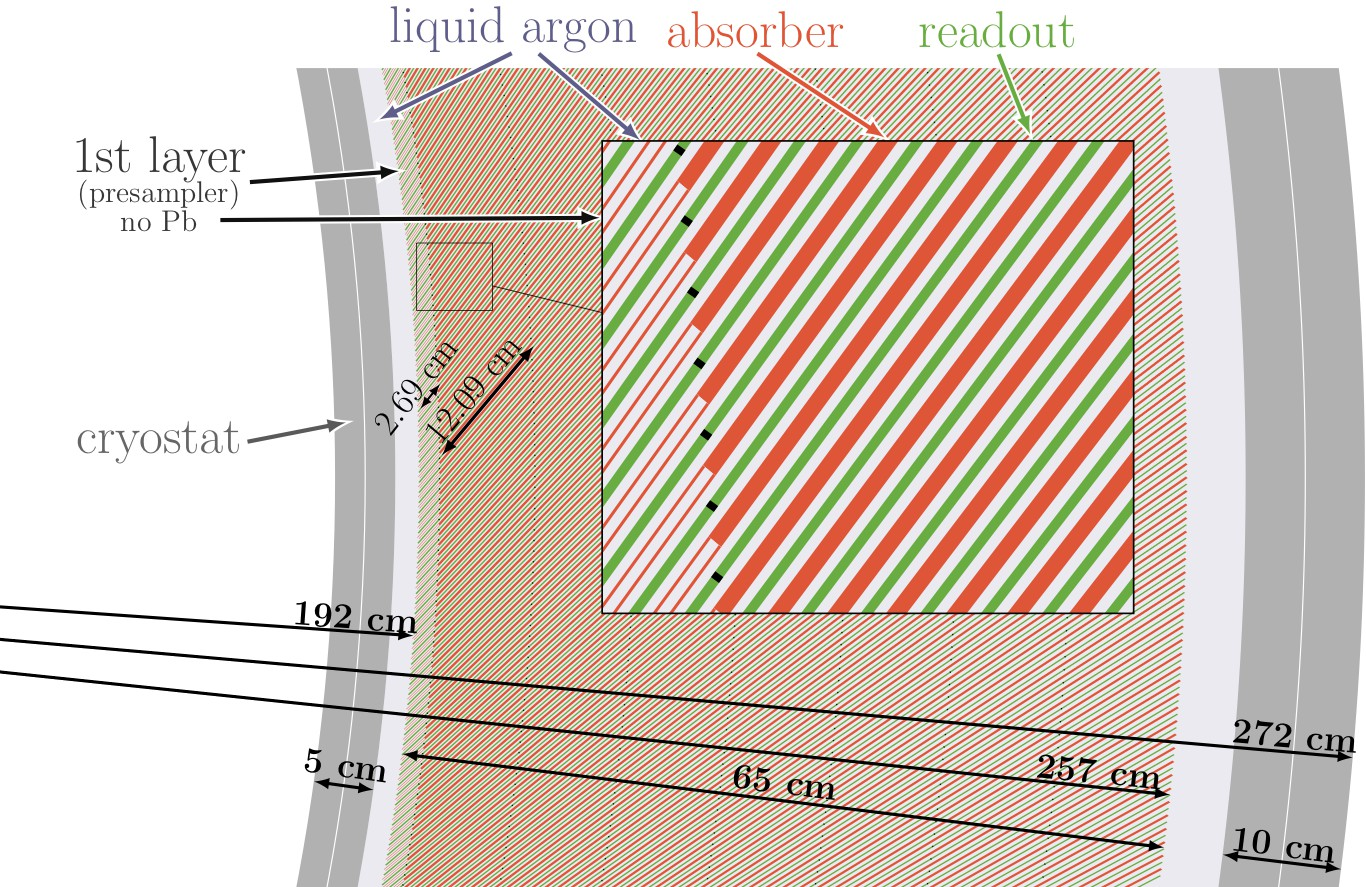
\includegraphics[width=0.49\linewidth]{figures/lar_calo_fcchh.png}
  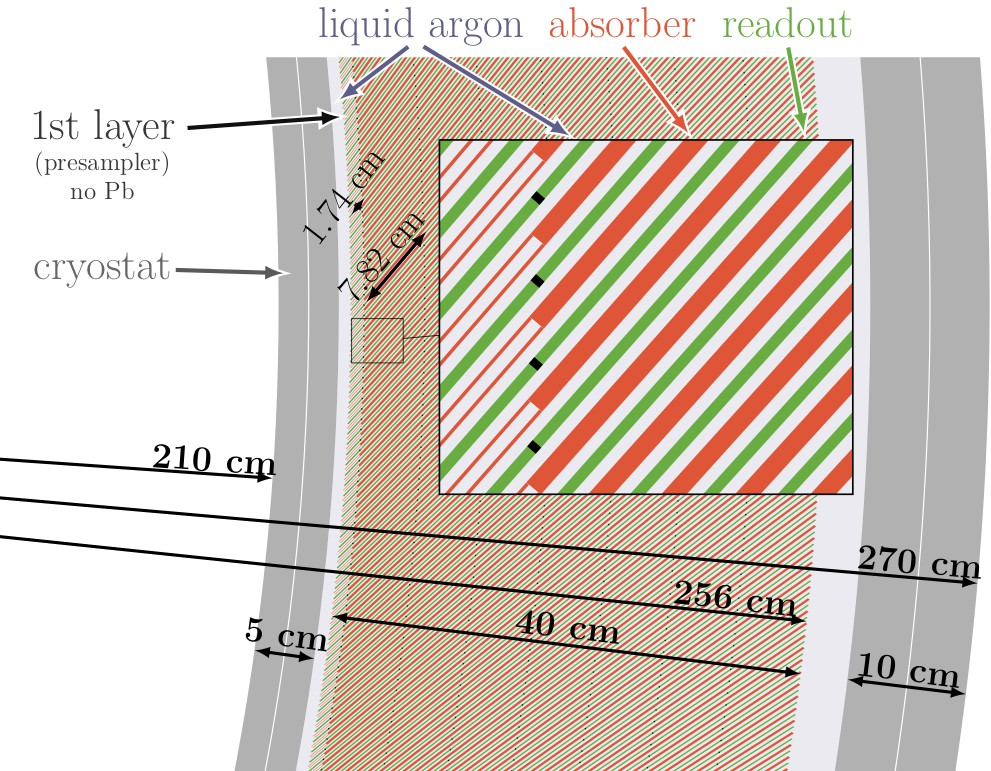
\includegraphics[width=0.49\linewidth]{figures/lar_calo_fccee.png}

  {\tiny
   \href{https://indico.cern.ch/event/969249/contributions/4086276/attachments/2132741/3591642/20201029_LAr_workingMeeting_Brieuc.pdf}
        {source: Brieuc François (CERN)}}
\end{frame}

% \begin{frame}
%   \frametitle{FCC-ee LAr Calorimeter Thickness}
% 
%   \begin{columns}[c]
%     \column{.4\textwidth}
%     LAr Thickness at $\theta = \pi/2$:
%     \begin{itemize}
%       \small
%       \item No cryostat: 21.5 $X_0$
%       \item With cryostat: 23.2 $X_0$
%     \end{itemize}
% 
%     \column{.6\textwidth}
%     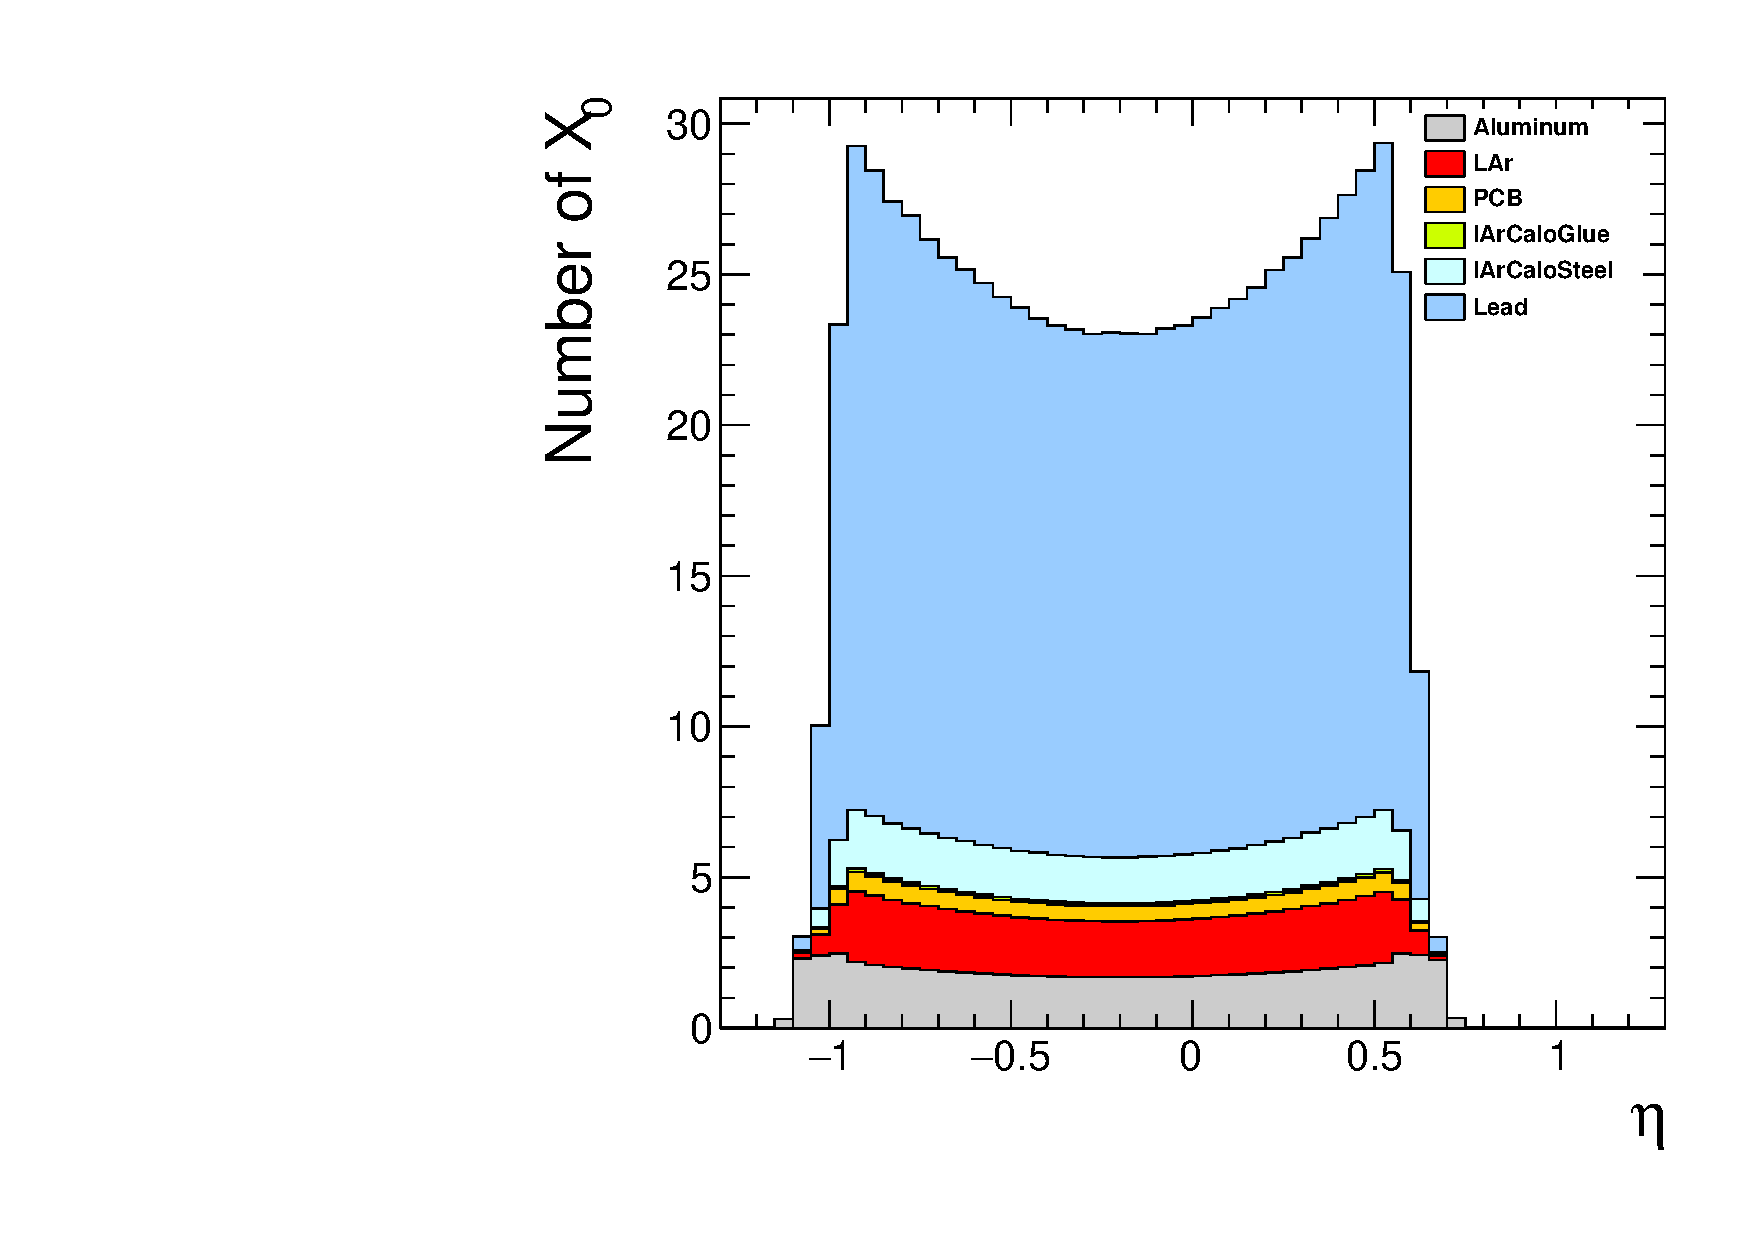
\includegraphics[width=\linewidth]{figures/x0.pdf}
%   \end{columns}
% \end{frame}


% ---------------------------------------------------------------------------- %
\section{Energy deposits outside calorimeter}

\begin{frame}
  \frametitle{FCC-ee: Energy deposits outside calorimeter I.}

  \begin{itemize}
    \item Energy is deposited also outside calorimeter, most notably in front
          and back cryostat
    \item There is correlation between first calorimeter layer and energy
          deposited in front cryostat
    \item Similarly, there is correlation between last calorimeter layer and
          energy deposited in back cryostat
    \item Energy deposited in side cryostats negligible \\
          (< 0.003 GeV for $e^{-}$, 100 GeV, $\theta = \pi/2$)
    \item Those correlations are exploited to create \redtext{upstream}
          and \redtext{downstream} energy corrections
    \item \bluetext{\bf This presentation:}
          \begin{itemize}
            \item \bluetext{\bf Corrections derived for 12 layer version of FCC-ee LAr
              Calorimeter (Merged Brieuc's branch)} \redtext{(Code was not yet
              transfered to FCCDetectors repository)}
            \item \bluetext{\bf Back cryostat extended to 1100~mm}
          \end{itemize}
  \end{itemize}
\end{frame}

\begin{frame}
  \frametitle{FCC-ee: Energy deposits outside calorimeter II.}

  \centering
  FCC-ee, $e^{-}$, \redtext{20 GeV}, \bluetext{$\theta = 70^{\circ}$} \\[1.2ex]
  \begin{adjustwidth}{-5mm}{-5mm}
    \includegraphics[width=0.49\linewidth]{figures/2d/hist_upstream_vs_layer_0_70deg_20GeV.pdf}
    \includegraphics[width=0.49\linewidth]{figures/2d/profile_upstream_vs_layer_0_70deg_20GeV.pdf}
  \end{adjustwidth}
  \redtext{Upstream} energy vs.\ energy in first layer
\end{frame}

\begin{frame}
  \frametitle{FCC-ee: Energy deposits outside calorimeter III.}

  \centering
  FCC-ee, $e^{-}$, \redtext{100 GeV}, \bluetext{$\theta = 70^{\circ}$} \\[1.5ex]
  \begin{adjustwidth}{-5mm}{-5mm}
    \includegraphics[width=0.49\linewidth]{figures/2d/hist_upstream_vs_layer_0_70deg_100GeV.pdf}
    \includegraphics[width=0.49\linewidth]{figures/2d/profile_upstream_vs_layer_0_70deg_100GeV.pdf}
  \end{adjustwidth}
  \redtext{Upstream} energy vs.\ energy in first layer
\end{frame}

\begin{frame}
  \frametitle{FCC-ee: Energy deposits outside calorimeter IV.}

  \centering
  FCC-ee, $e^{-}$, \redtext{240 GeV}, \bluetext{$\theta = 70^{\circ}$} \\[1.5ex]
  \begin{adjustwidth}{-5mm}{-5mm}
    \includegraphics[width=0.49\linewidth]{figures/2d/hist_upstream_vs_layer_0_70deg_240GeV.pdf}
    \includegraphics[width=0.49\linewidth]{figures/2d/profile_upstream_vs_layer_0_70deg_240GeV.pdf}
  \end{adjustwidth}
  \redtext{Upstream} energy vs.\ energy in first layer
\end{frame}

\begin{frame}
  \frametitle{FCC-ee: Energy deposits outside calorimeter V.}

  \centering
  FCC-ee, $e^{-}$, \redtext{20 GeV}, \bluetext{$\theta = 70^{\circ}$} \\[1.5ex]
  \begin{adjustwidth}{-5mm}{-5mm}
    \includegraphics[width=0.49\linewidth]{figures/2d/hist_downstream_vs_layer_11_70deg_20GeV.pdf}
    \includegraphics[width=0.49\linewidth]{figures/2d/profile_downstream_vs_layer_11_70deg_20GeV.pdf}
  \end{adjustwidth}
  \redtext{Downstream} energy vs.\ energy in last layer
\end{frame}

\begin{frame}
  \frametitle{FCC-ee: Energy deposits outside calorimeter VI.}

  \centering
  FCC-ee, $e^{-}$, \redtext{100 GeV}, \bluetext{$\theta = 70^{\circ}$} \\[1.5ex]
  \begin{adjustwidth}{-5mm}{-5mm}
    \includegraphics[width=0.49\linewidth]{figures/2d/hist_downstream_vs_layer_11_70deg_100GeV.pdf}
    \includegraphics[width=0.49\linewidth]{figures/2d/profile_downstream_vs_layer_11_70deg_100GeV.pdf}
  \end{adjustwidth}
  \redtext{Downstream} energy vs.\ energy in last layer
\end{frame}

\begin{frame}
  \frametitle{FCC-ee: Energy deposits outside calorimeter VII.}

  \centering
  FCC-ee, $e^{-}$, \redtext{240 GeV}, \bluetext{$\theta = 70^{\circ}$} \\[1.5ex]
  \begin{adjustwidth}{-5mm}{-5mm}
    \includegraphics[width=0.49\linewidth]{figures/2d/hist_downstream_vs_layer_11_70deg_240GeV.pdf}
    \includegraphics[width=0.49\linewidth]{figures/2d/profile_downstream_vs_layer_11_70deg_240GeV.pdf}
  \end{adjustwidth}
  \redtext{Downstream} energy vs.\ energy in last layer
\end{frame}

\begin{frame}
  \frametitle{FCC-ee: Upstream Energy vs. First Layer}

  \centering
  \redtext{Cluster energy dependence} \\[1.5ex]
  \begin{adjustwidth}{-5mm}{-5mm}
    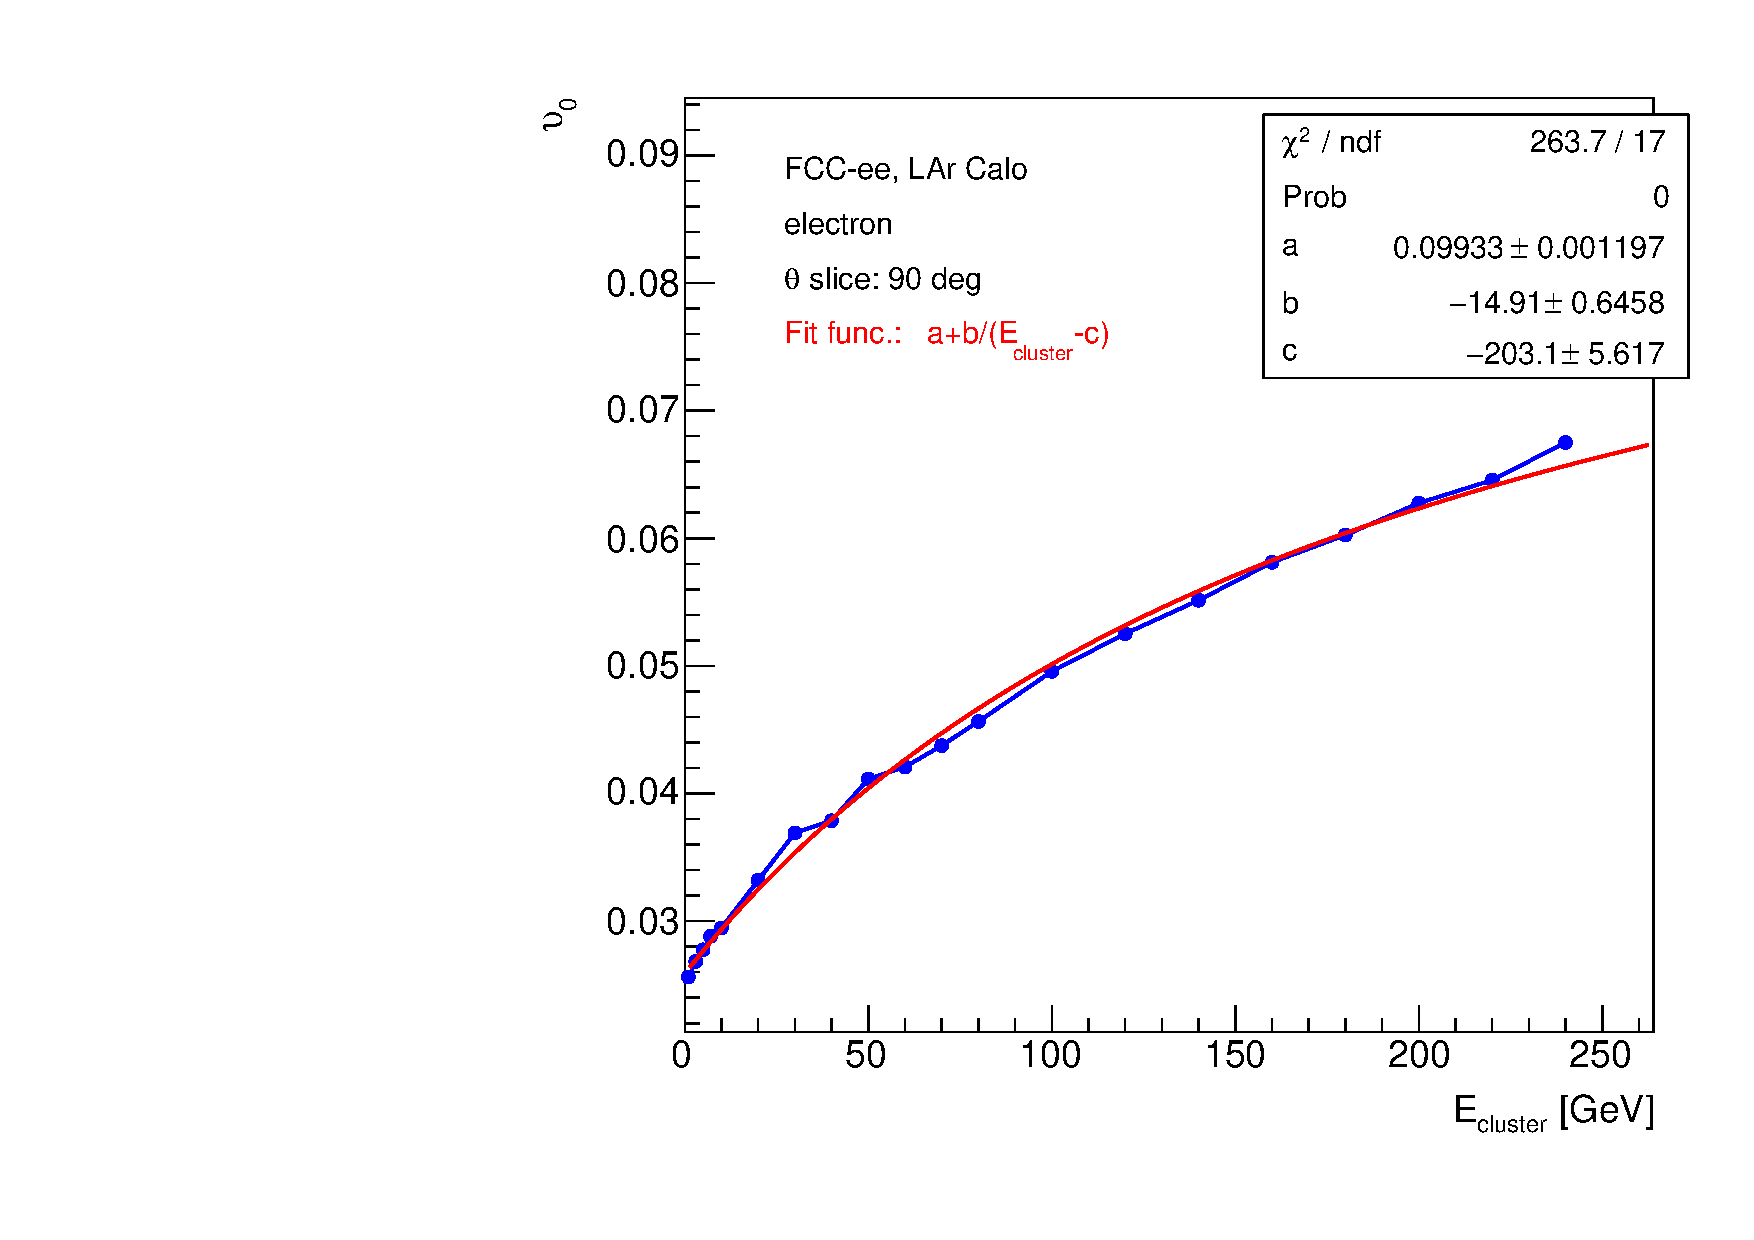
\includegraphics[width=0.49\linewidth]{figures/2d/graph_upstream_energy_upsilon_0.pdf}
    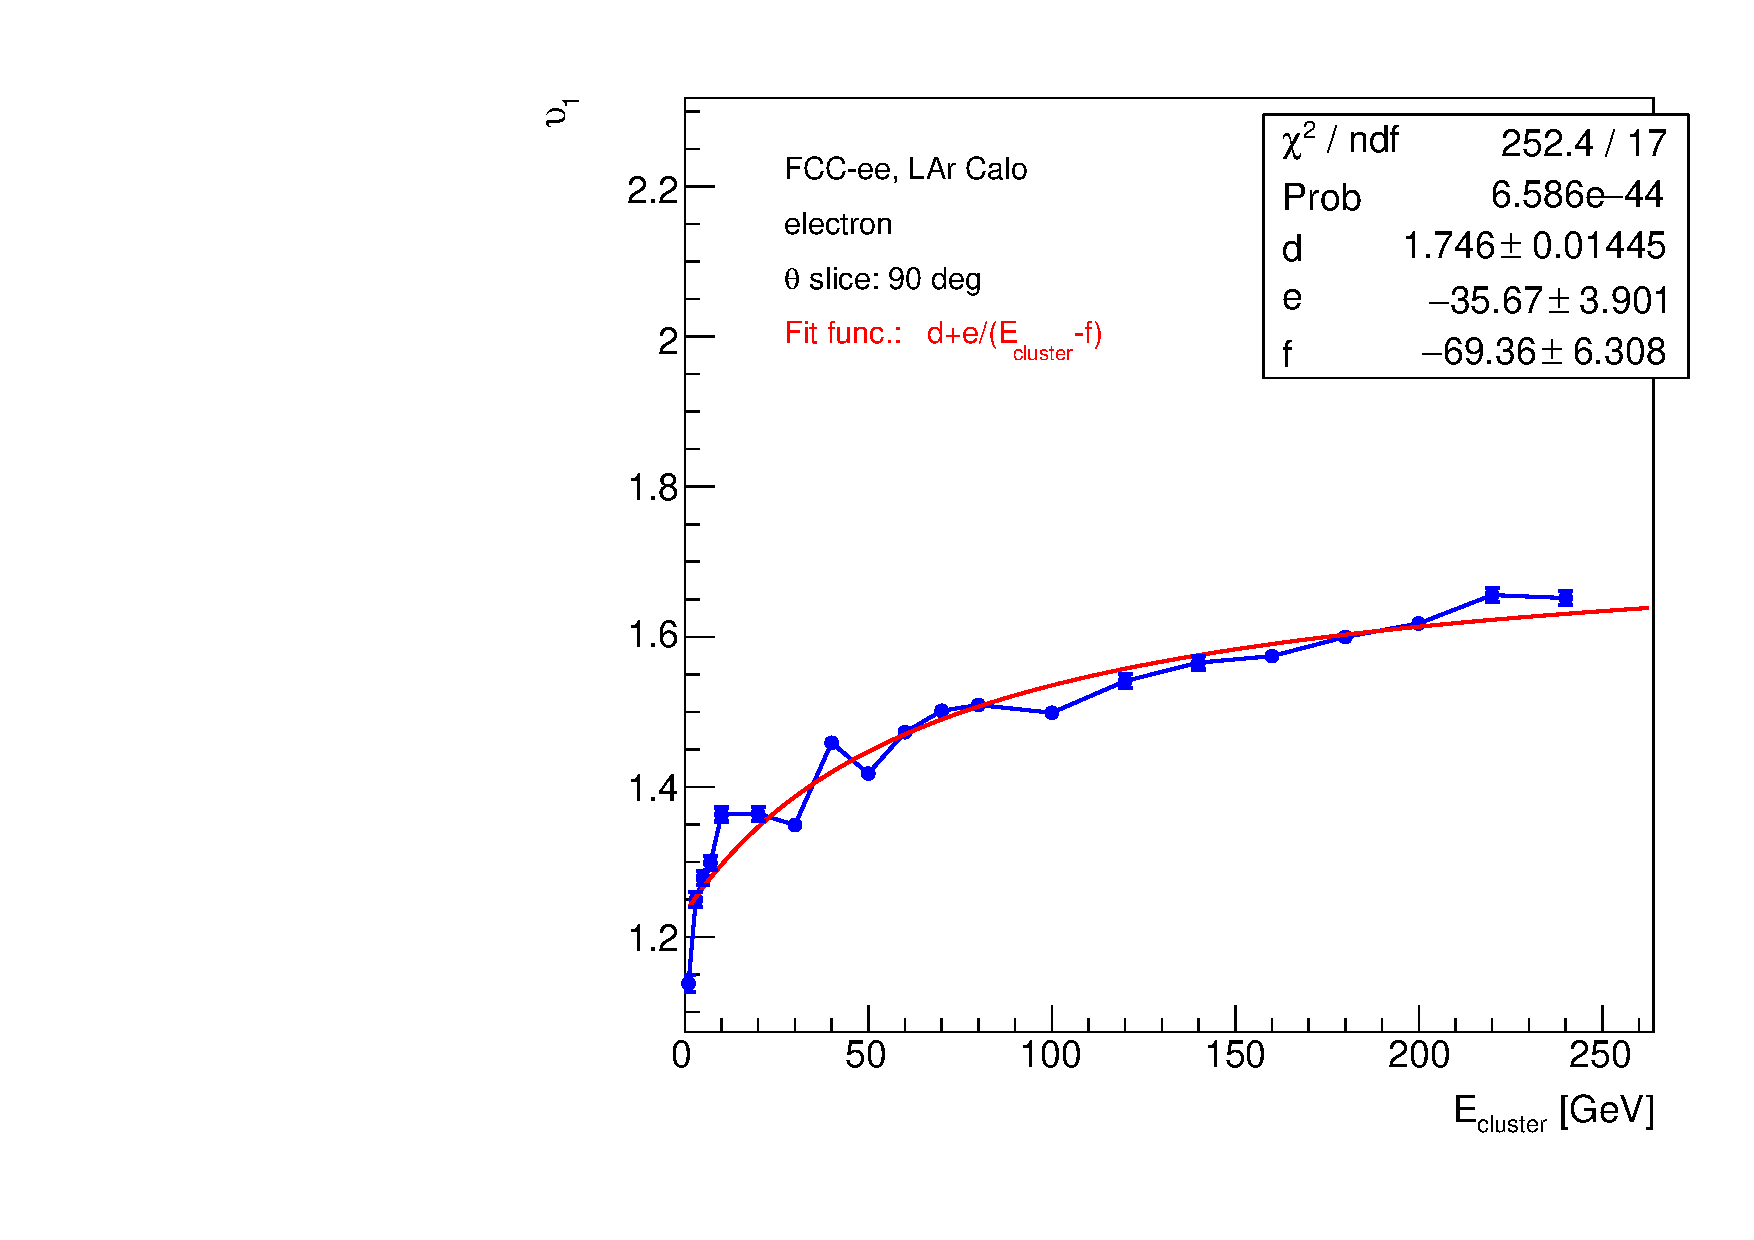
\includegraphics[width=0.49\linewidth]{figures/2d/graph_upstream_energy_upsilon_1.pdf}\\[-3ex]
  \end{adjustwidth}
\end{frame}

\begin{frame}
  \frametitle{FCC-ee: Upstream Energy vs. First Layer}

  \centering
  \redtext{Cluster angle dependence} \\[1.5ex]
  \begin{adjustwidth}{-5mm}{-5mm}
    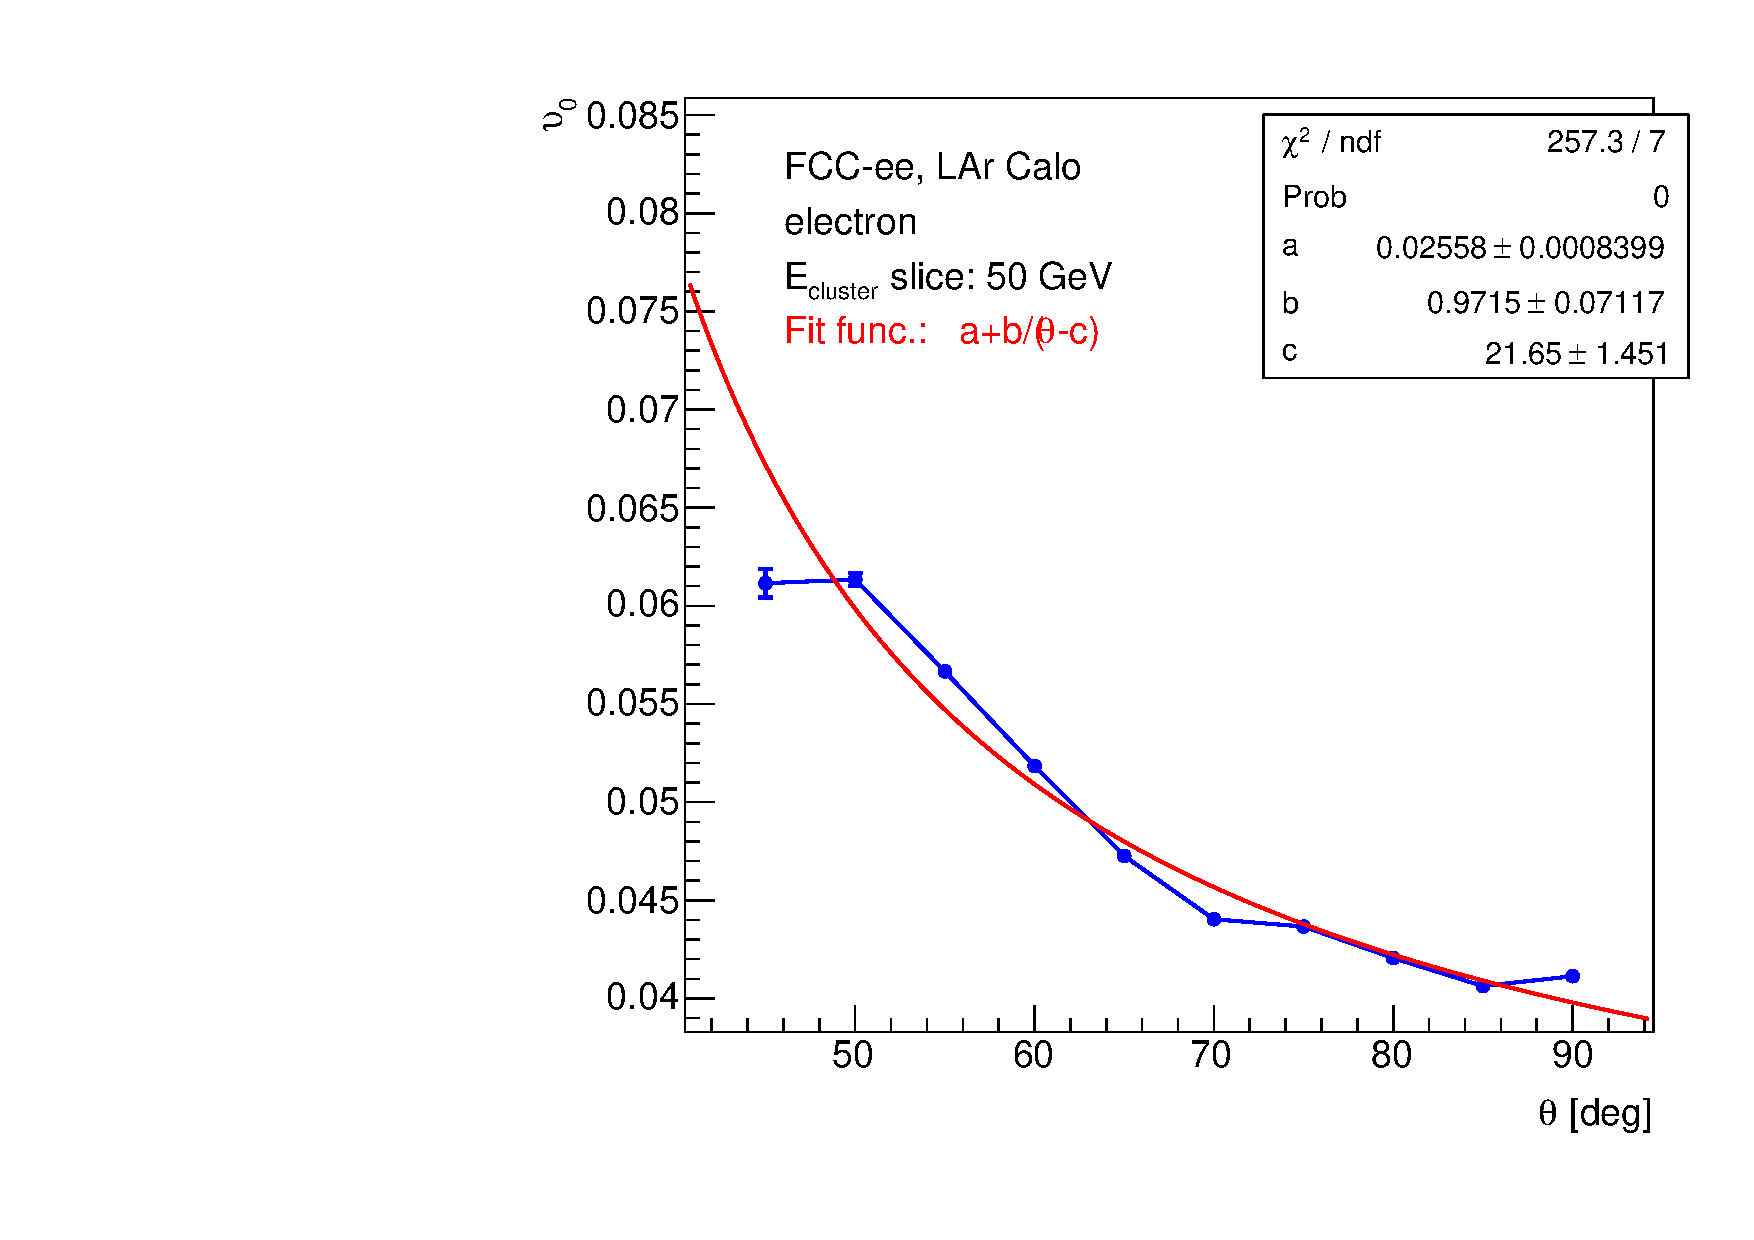
\includegraphics[width=0.49\linewidth]{figures/2d/graph_upstream_theta_upsilon_0.pdf}
    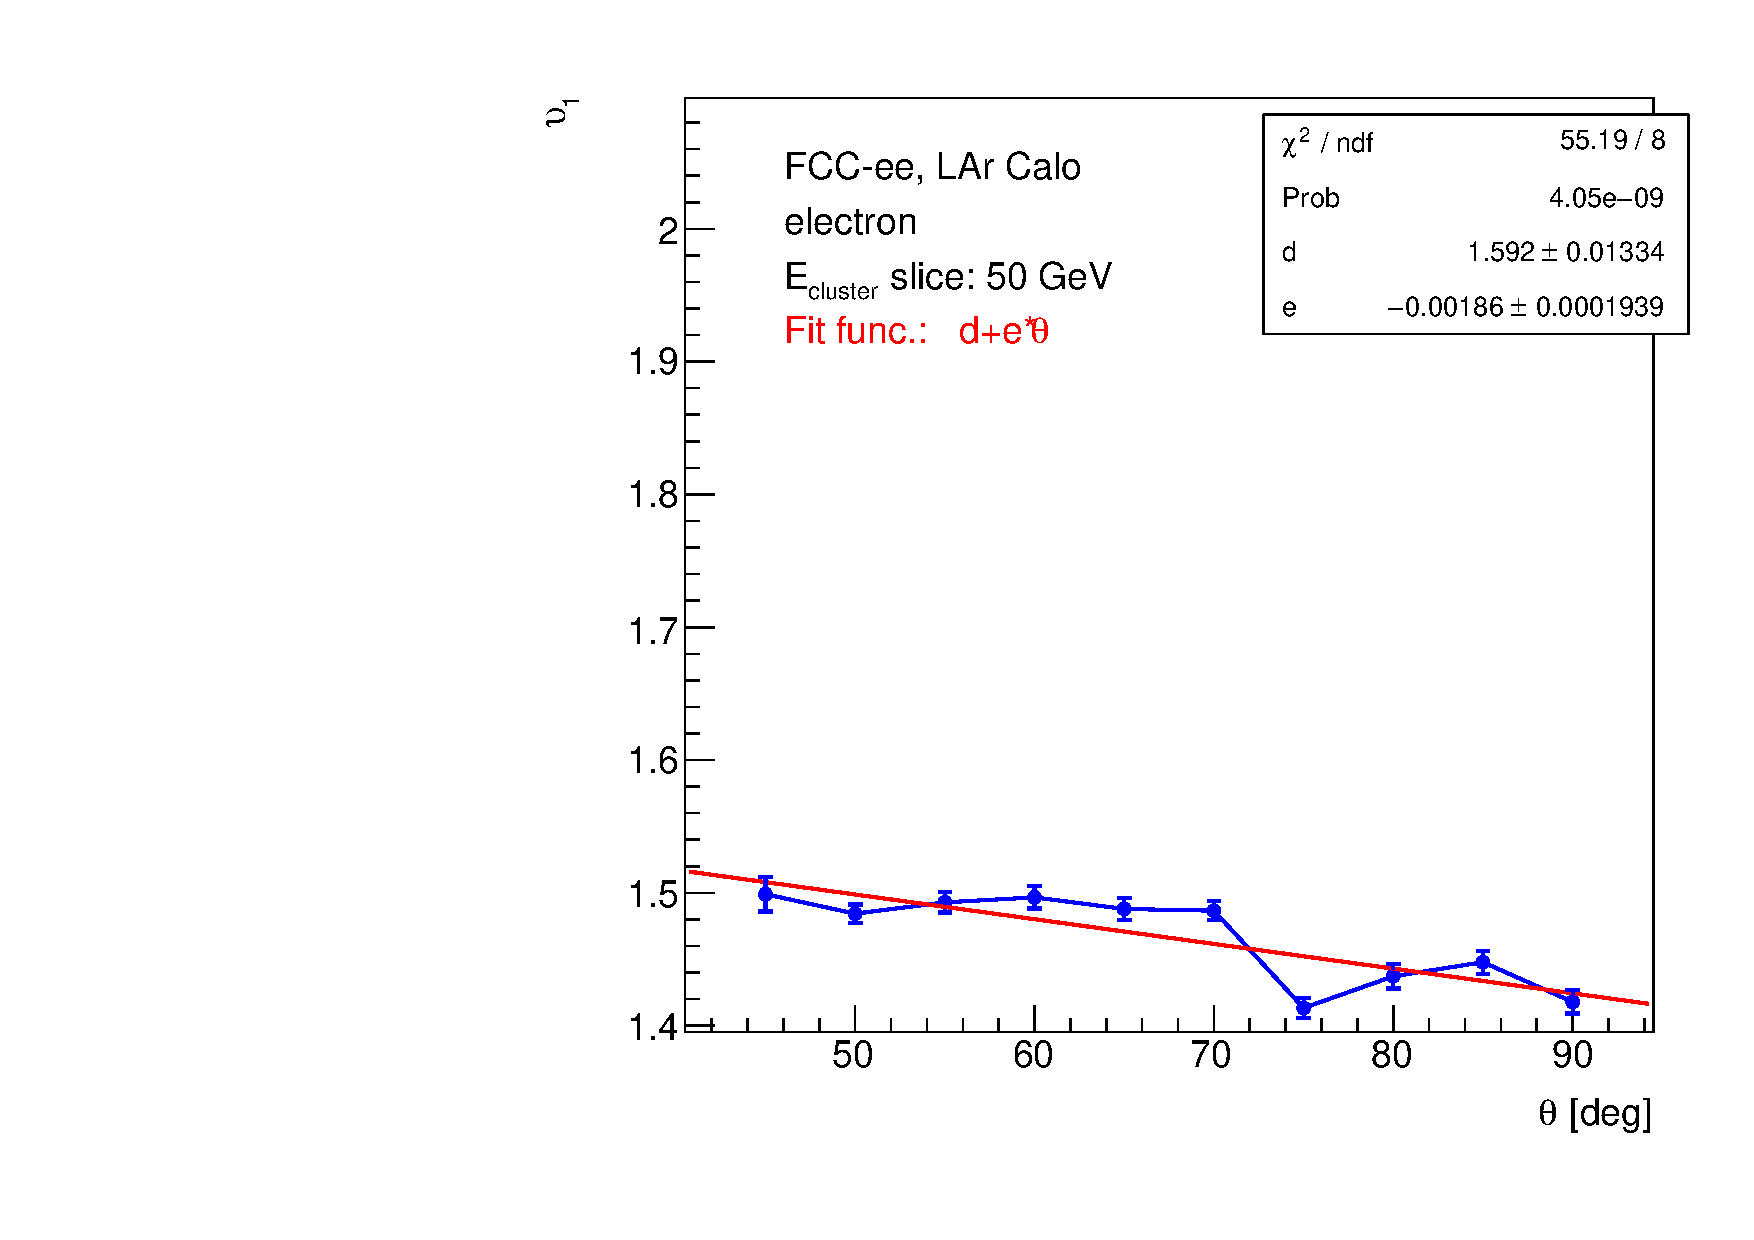
\includegraphics[width=0.49\linewidth]{figures/2d/graph_upstream_theta_upsilon_1.pdf}\\[-3ex]
  \end{adjustwidth}
\end{frame}

\begin{frame}
  \frametitle{FCC-ee: Downstream Energy vs. First Layer}

  \centering
  \redtext{Cluster energy dependence} \\[2.5ex]
  \begin{adjustwidth}{-5mm}{-5mm}
    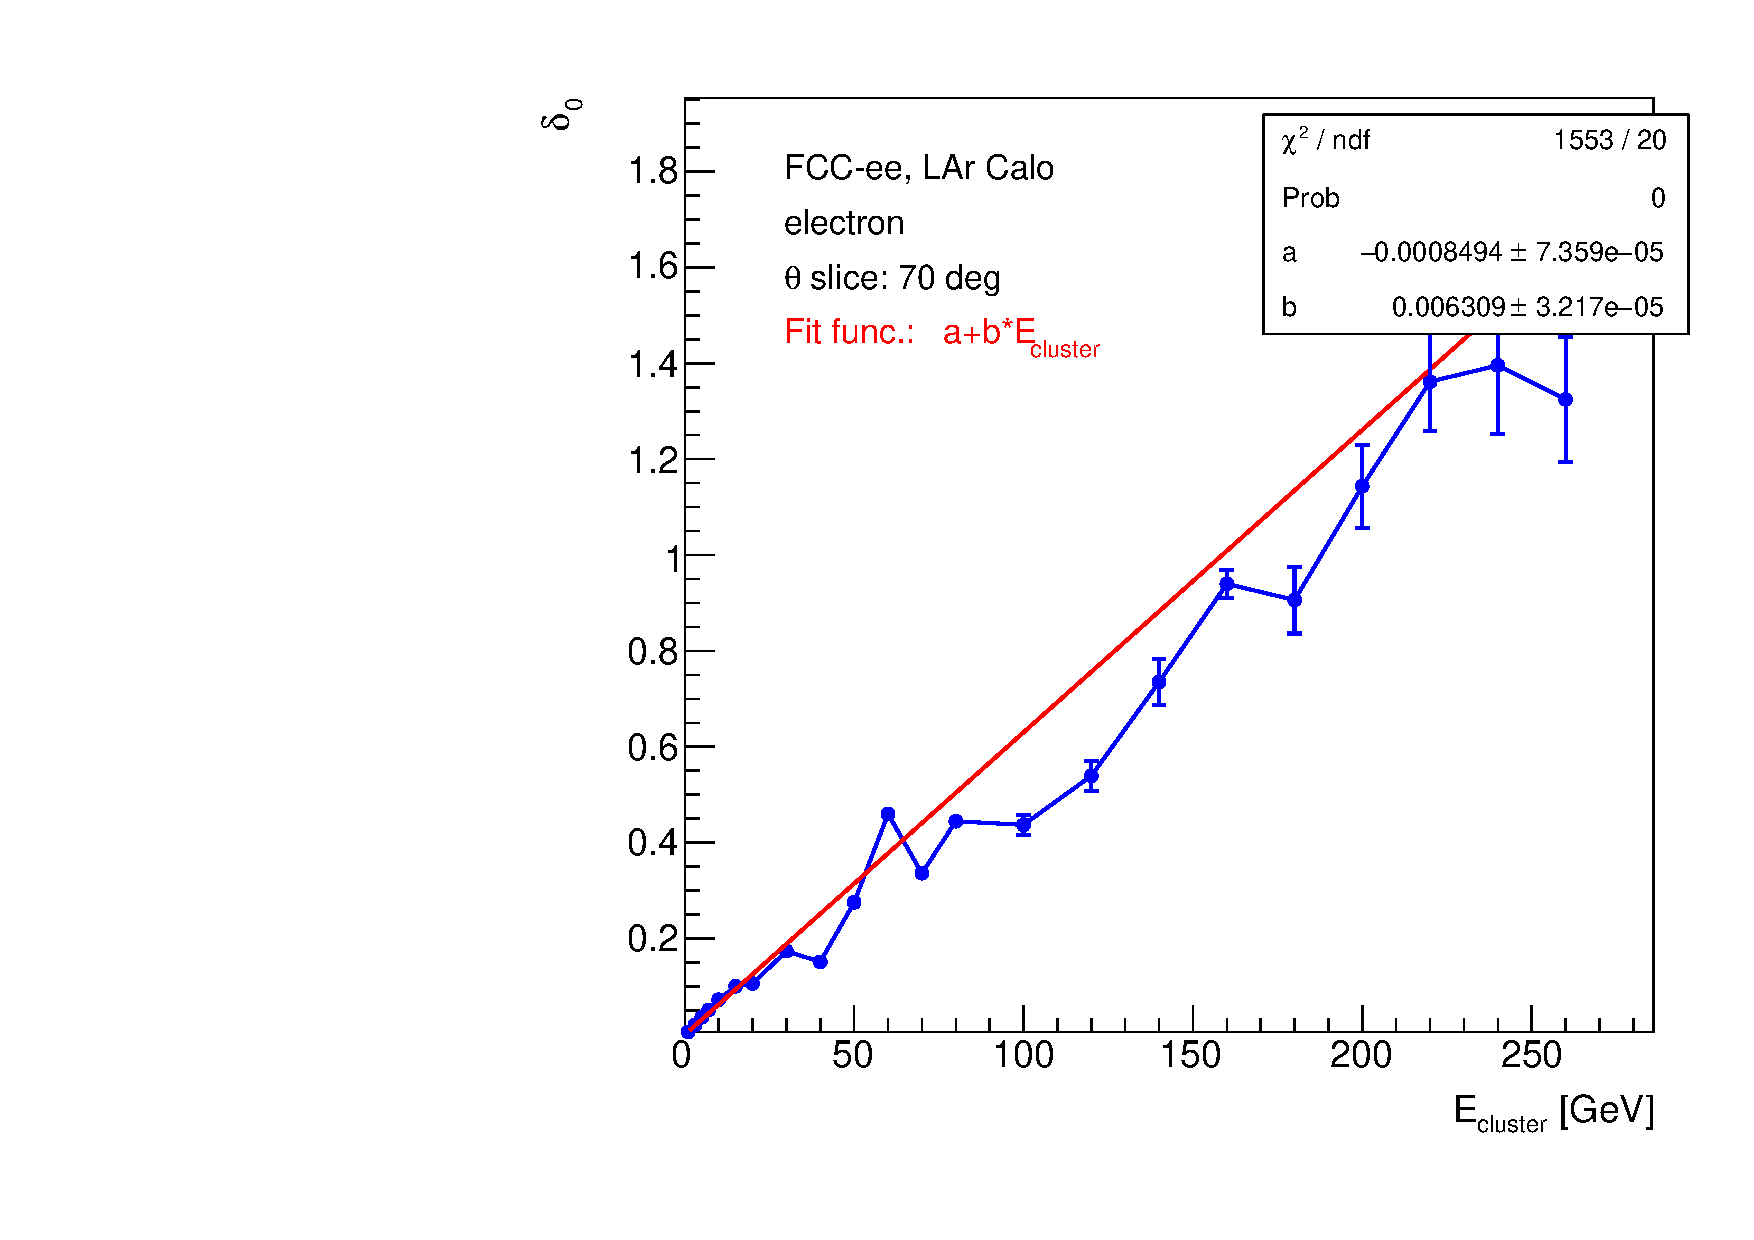
\includegraphics[width=0.32\linewidth]{figures/2d/graph_downstream_energy_delta_0_70deg.pdf}
    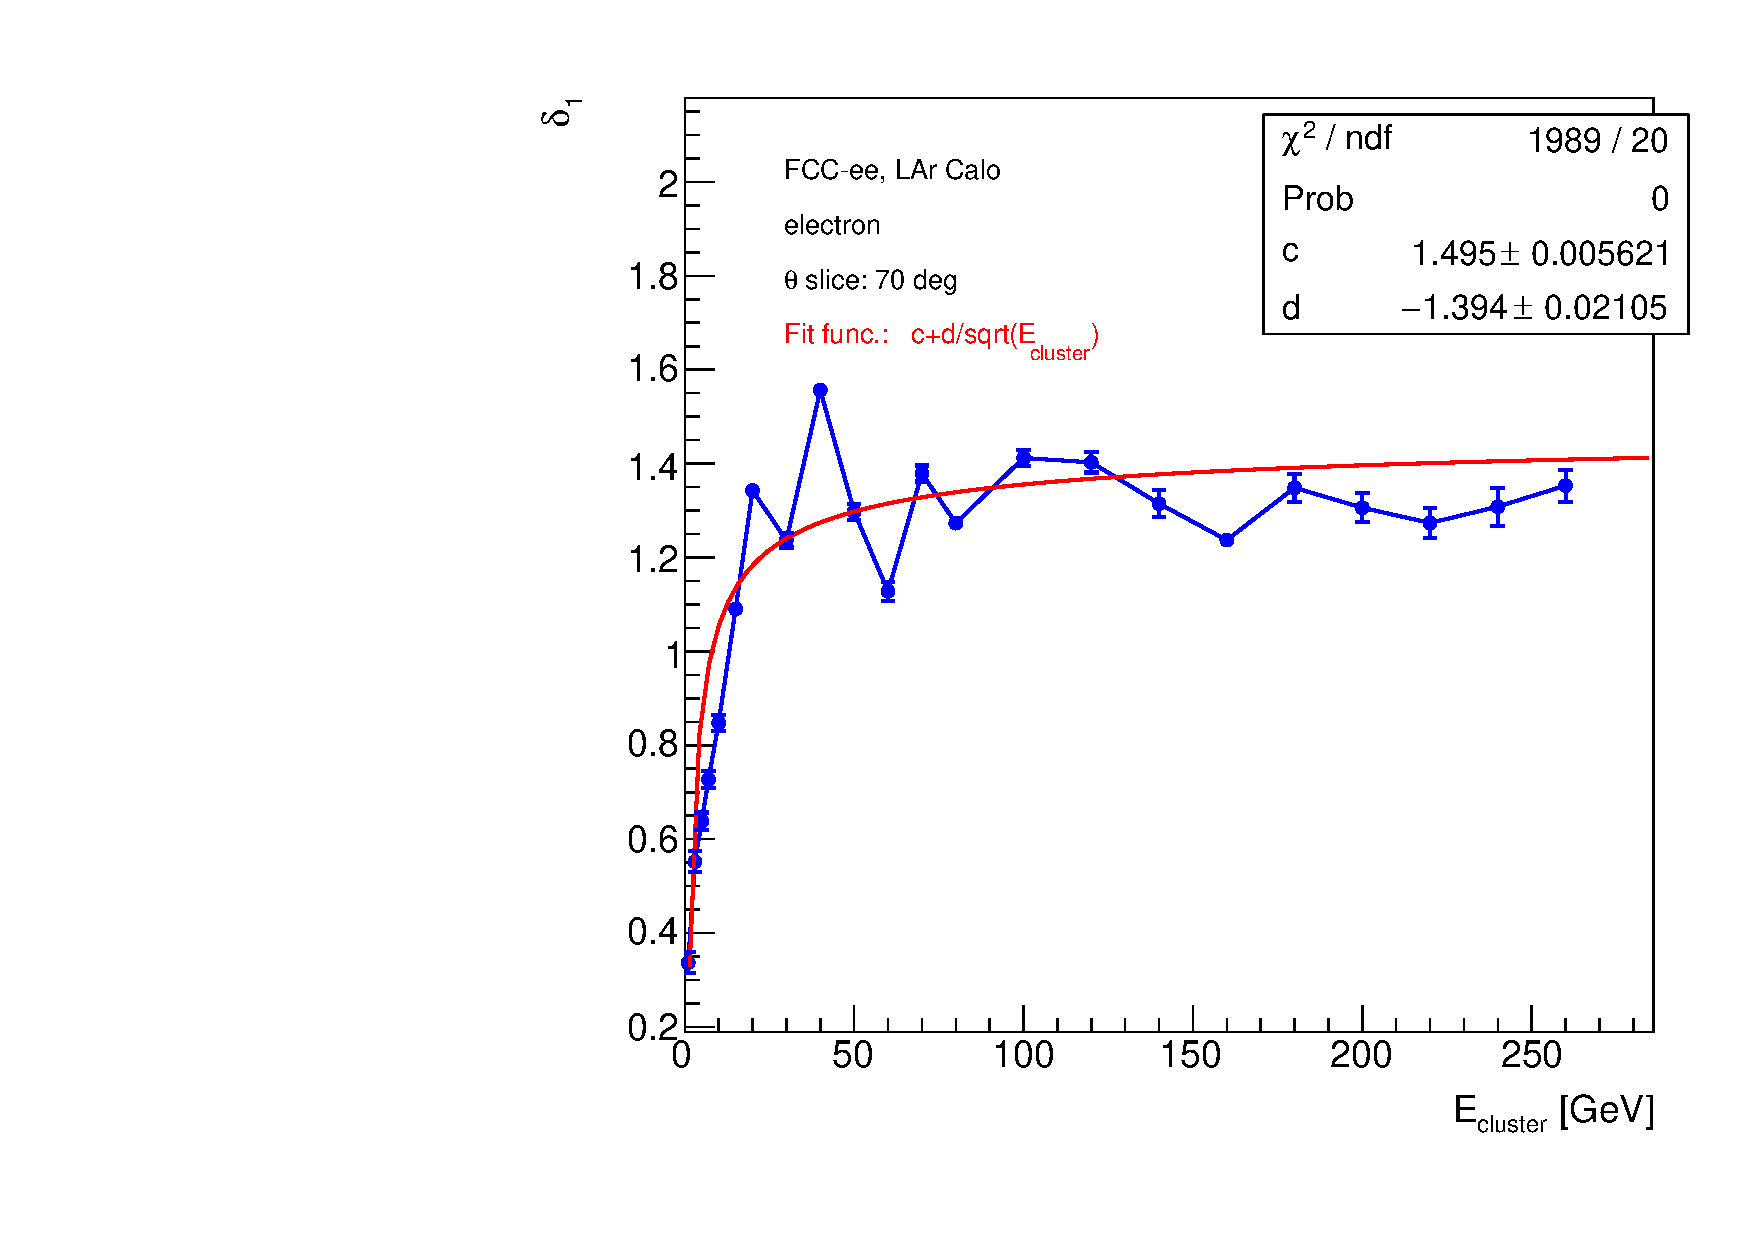
\includegraphics[width=0.32\linewidth]{figures/2d/graph_downstream_energy_delta_1_70deg.pdf}
    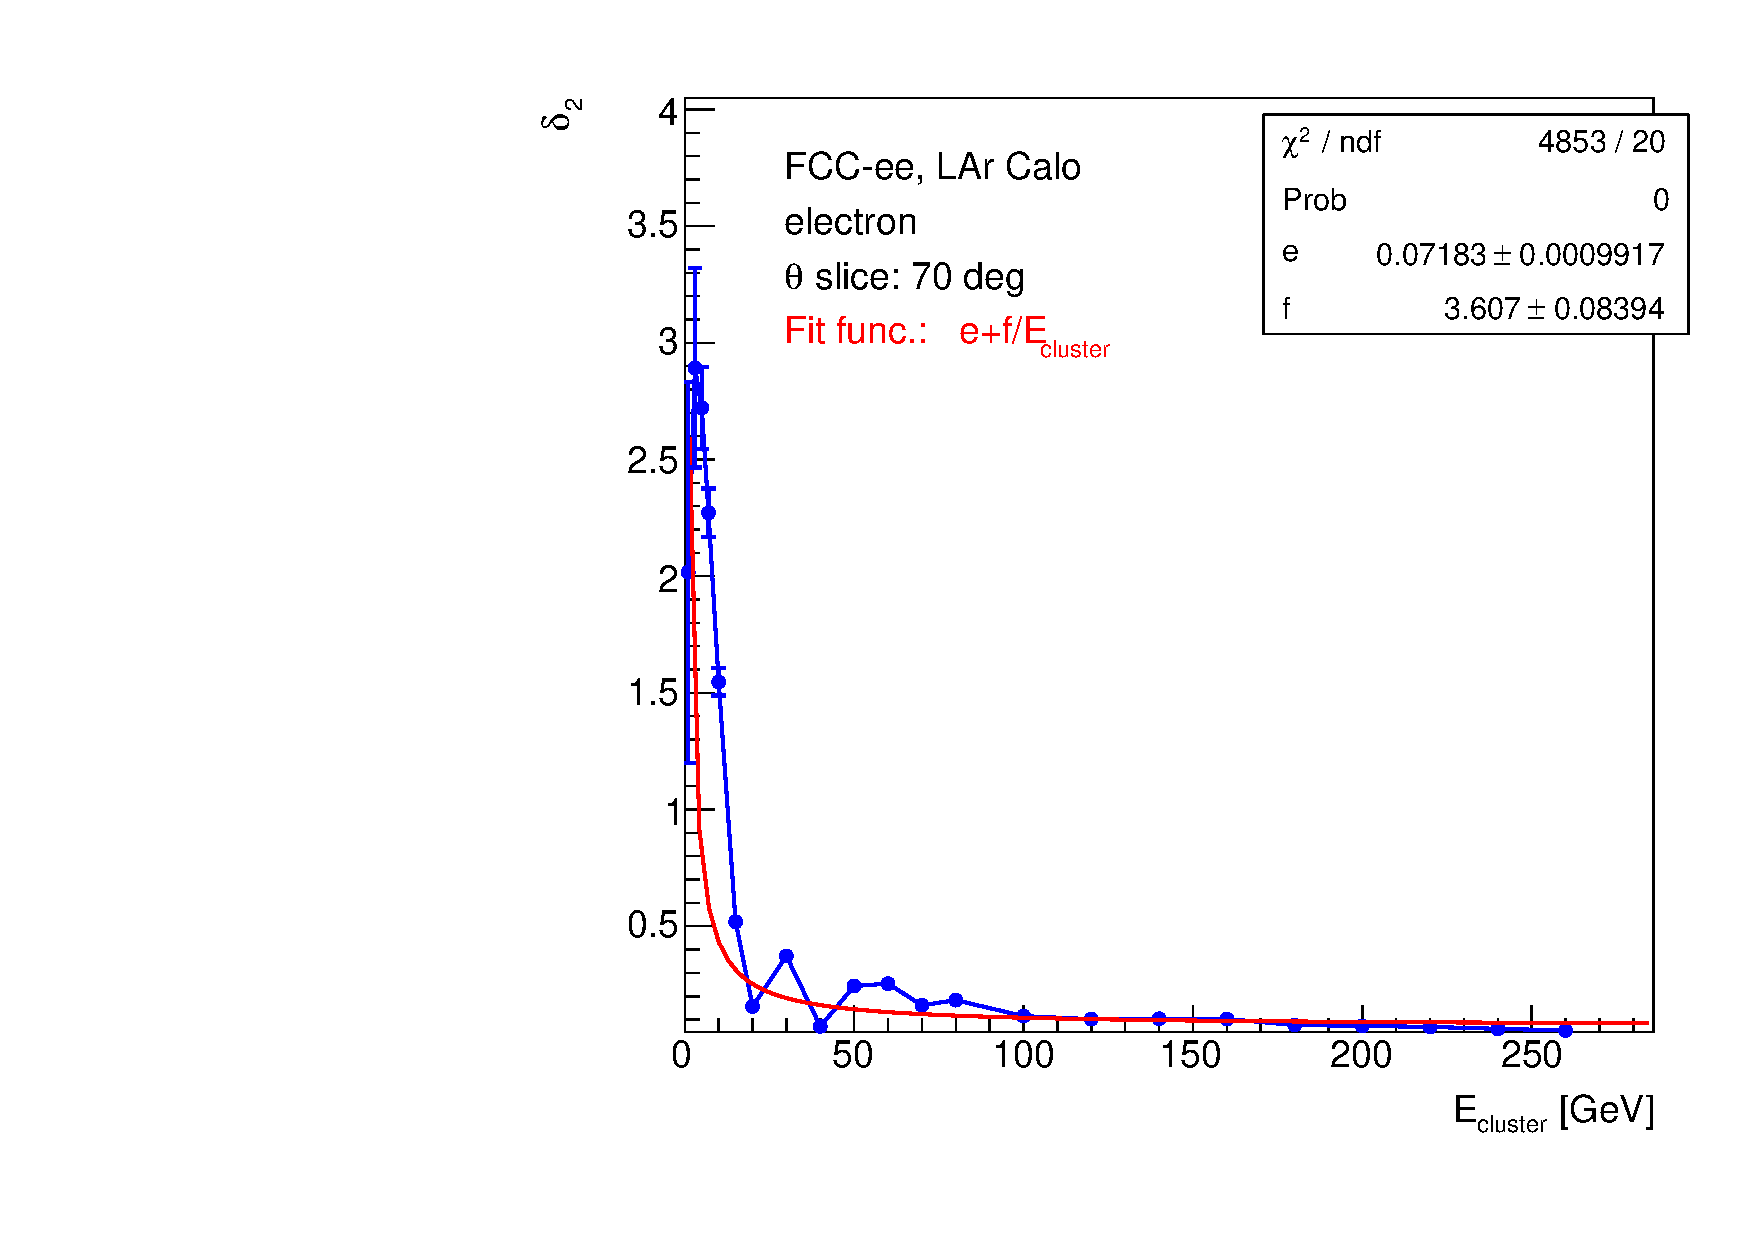
\includegraphics[width=0.32\linewidth]{figures/2d/graph_downstream_energy_delta_2_70deg.pdf}
  \end{adjustwidth}
  \bluetext{Cluster angle slice: 70 $^{\circ}$}
\end{frame}

\begin{frame}
  \frametitle{FCC-ee: Upstream Energy vs. First Layer}

  \centering
  \redtext{Cluster angle dependence} \\[1.5ex]
  \begin{adjustwidth}{-5mm}{-5mm}
    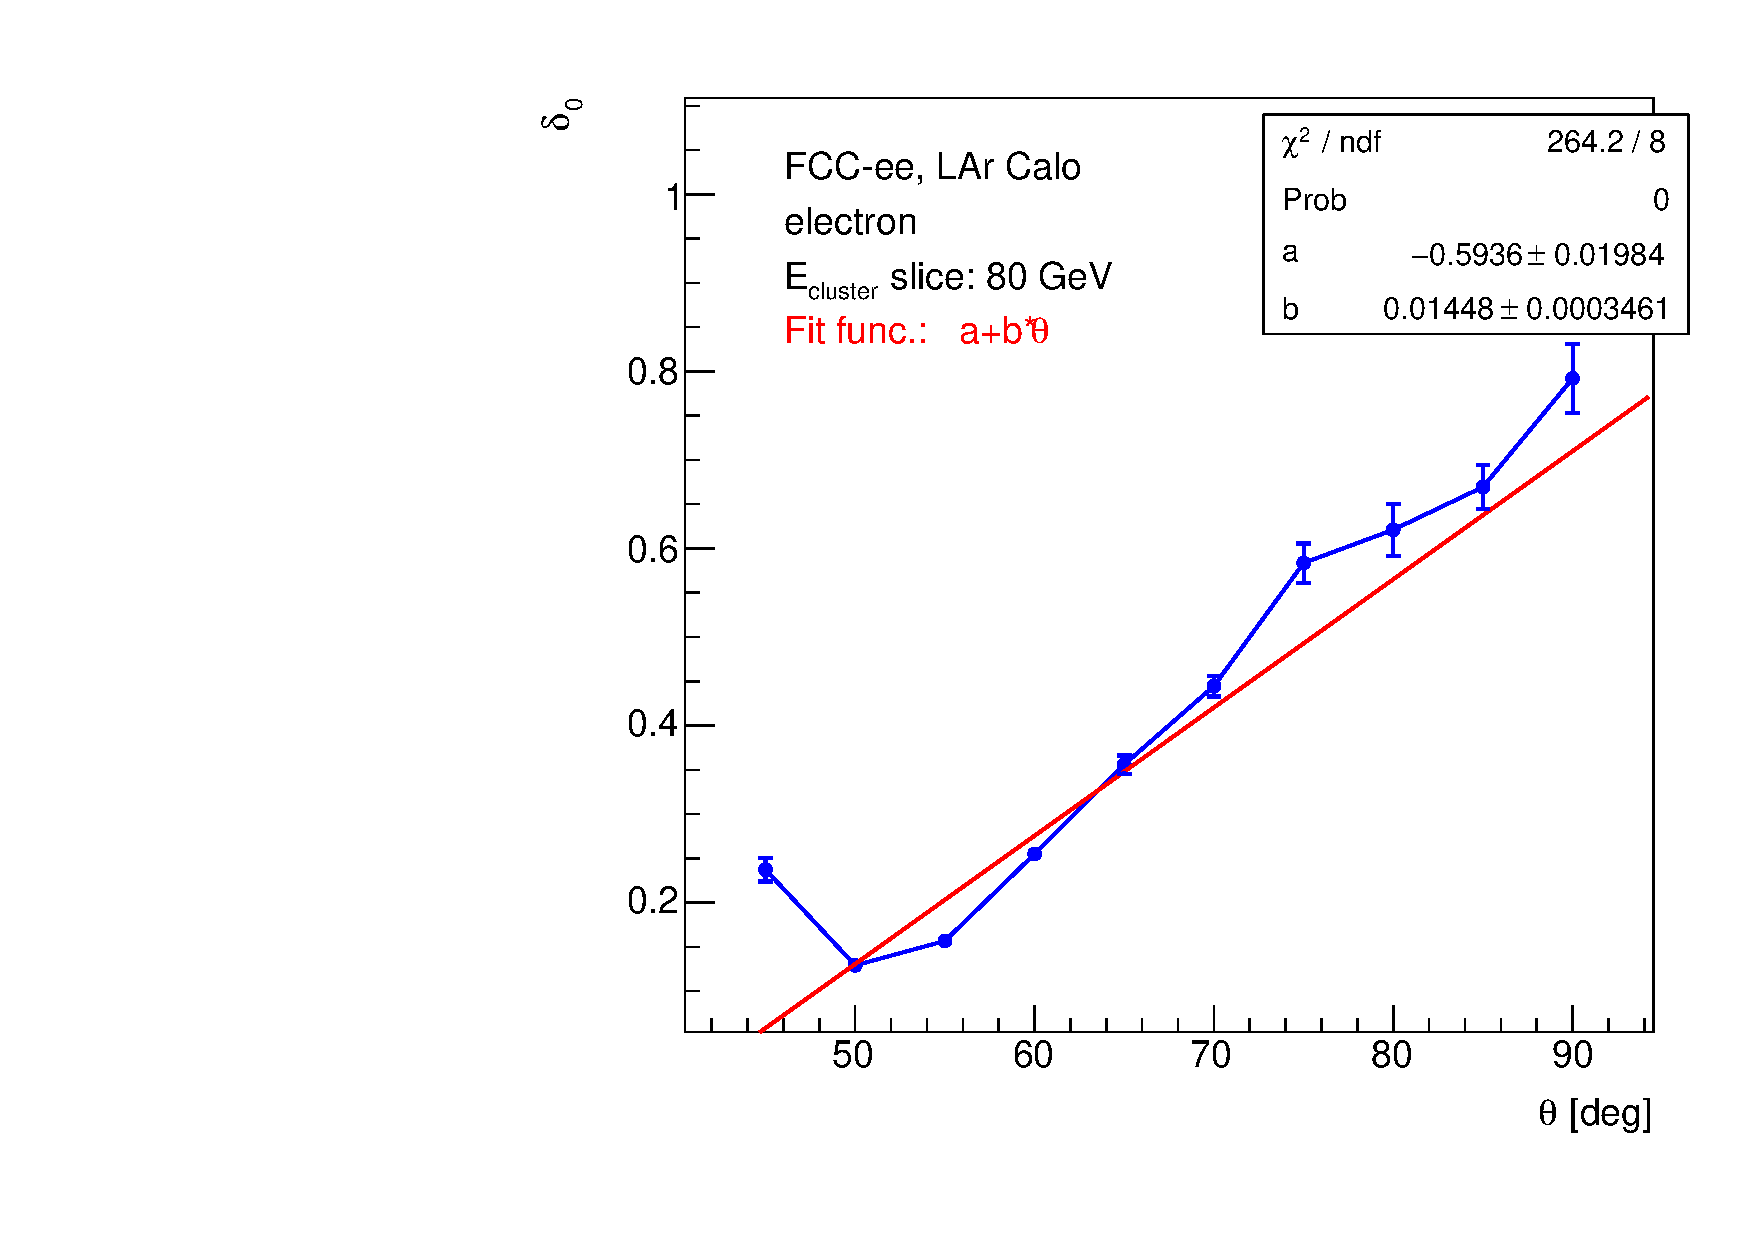
\includegraphics[width=0.32\linewidth]{figures/2d/graph_downstream_theta_delta_0_80gev.pdf}
    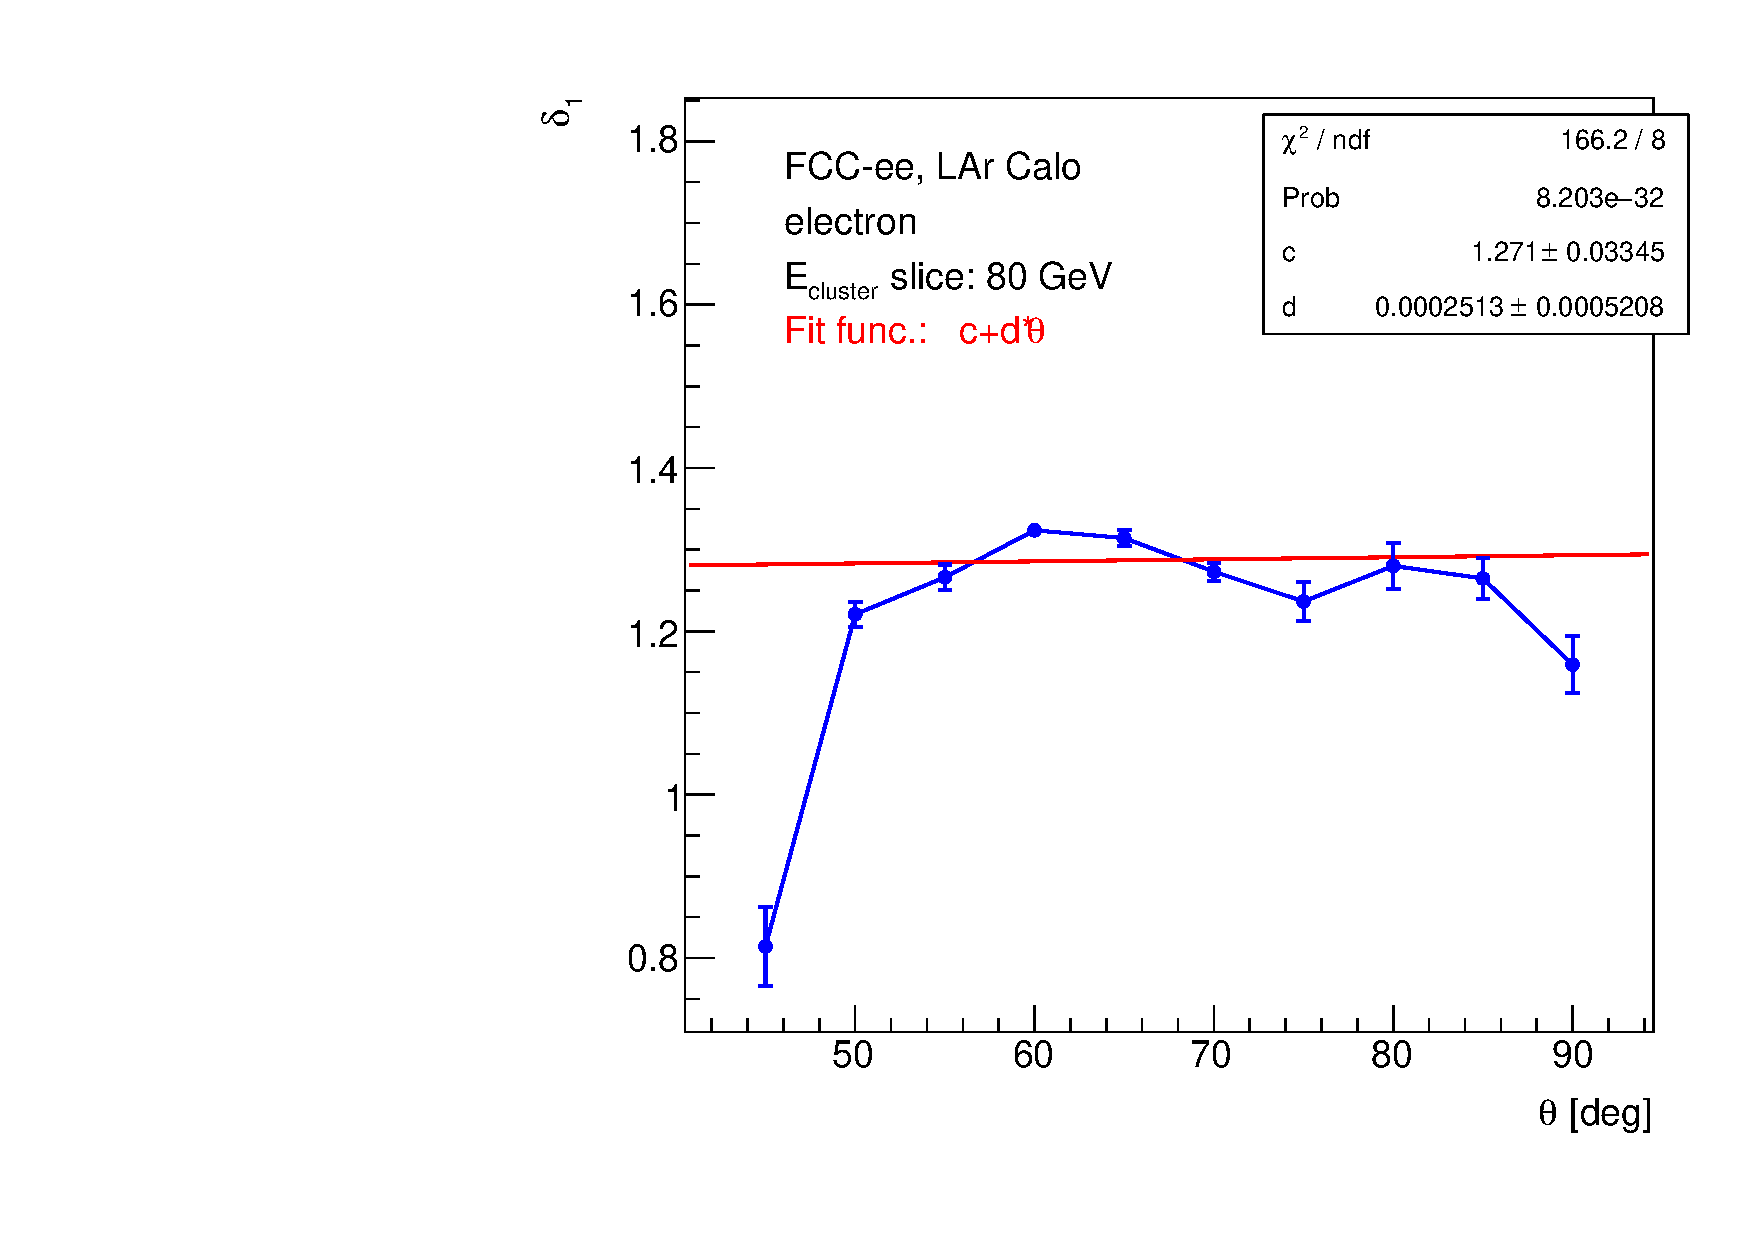
\includegraphics[width=0.32\linewidth]{figures/2d/graph_downstream_theta_delta_1_80gev.pdf}
    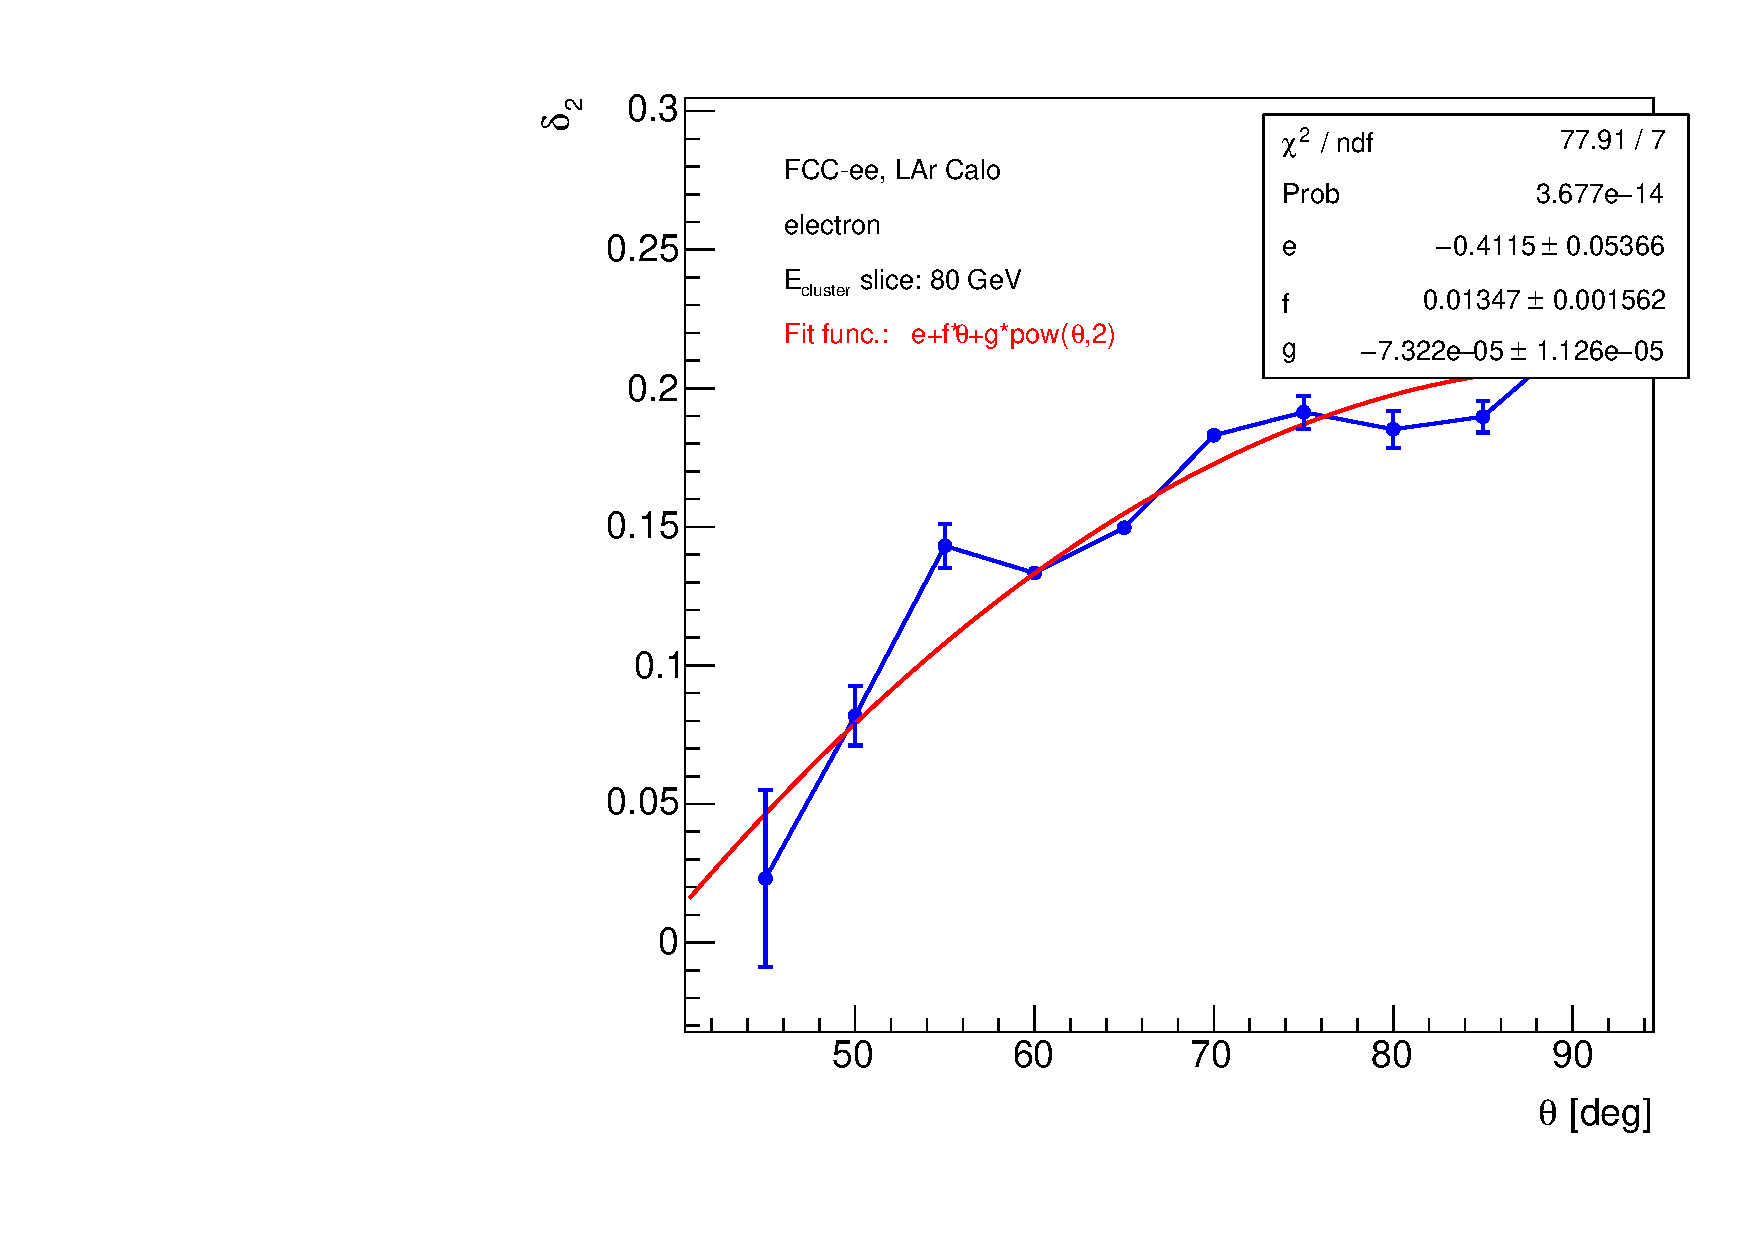
\includegraphics[width=0.32\linewidth]{figures/2d/graph_downstream_theta_delta_2_80gev.pdf}
  \end{adjustwidth}
\end{frame}


% ---------------------------------------------------------------------------- %
\section{Upstream Correction}

% \begin{frame}
%   \frametitle{Energy Correction at FCC-ee LAr Calorimeter (WIP)}
% 
%   \begin{equation*}
%     E = E_\text{upstream} + E_\text{downstream} + E_\text{cluster}
%   \end{equation*}
% 
%   \redtext{Upstream} parametrization:
%   \begin{equation*}
%   E_\text{upstream} = \upsilon_0 + \upsilon_1 \cdot E_\text{firstLayer}
%   \end{equation*}
%   \begin{equation*}
%     \upsilon_0 = a + b \cdot E_{cluster}  \qquad
%     \upsilon_1 = c + d \cdot E_{cluster}
%   \end{equation*}
% 
%   \redtext{Downstream} parametrization:
%   \begin{equation*}
%   E_\text{downstream} = \delta_0 \quad + \quad
%                         \delta_1 \cdot E_\text{lastLayer} \quad + \quad
%                         \delta_2 \cdot E_\text{lastLayer}^{2}
%   \end{equation*}
%   \begin{equation*}
%     \delta_0 = a + b \cdot E_{cluster}  \qquad
%     \delta_1 = c + \frac{d}{E_{cluster}} \qquad
%     \delta_2 = e + \frac{f}{E_{cluster}}
%   \end{equation*}
% \end{frame}

\begin{frame}
  \frametitle{FCC-ee Upstream Correction Energy Dependence}

  \begin{adjustwidth}{-9mm}{-9mm}
    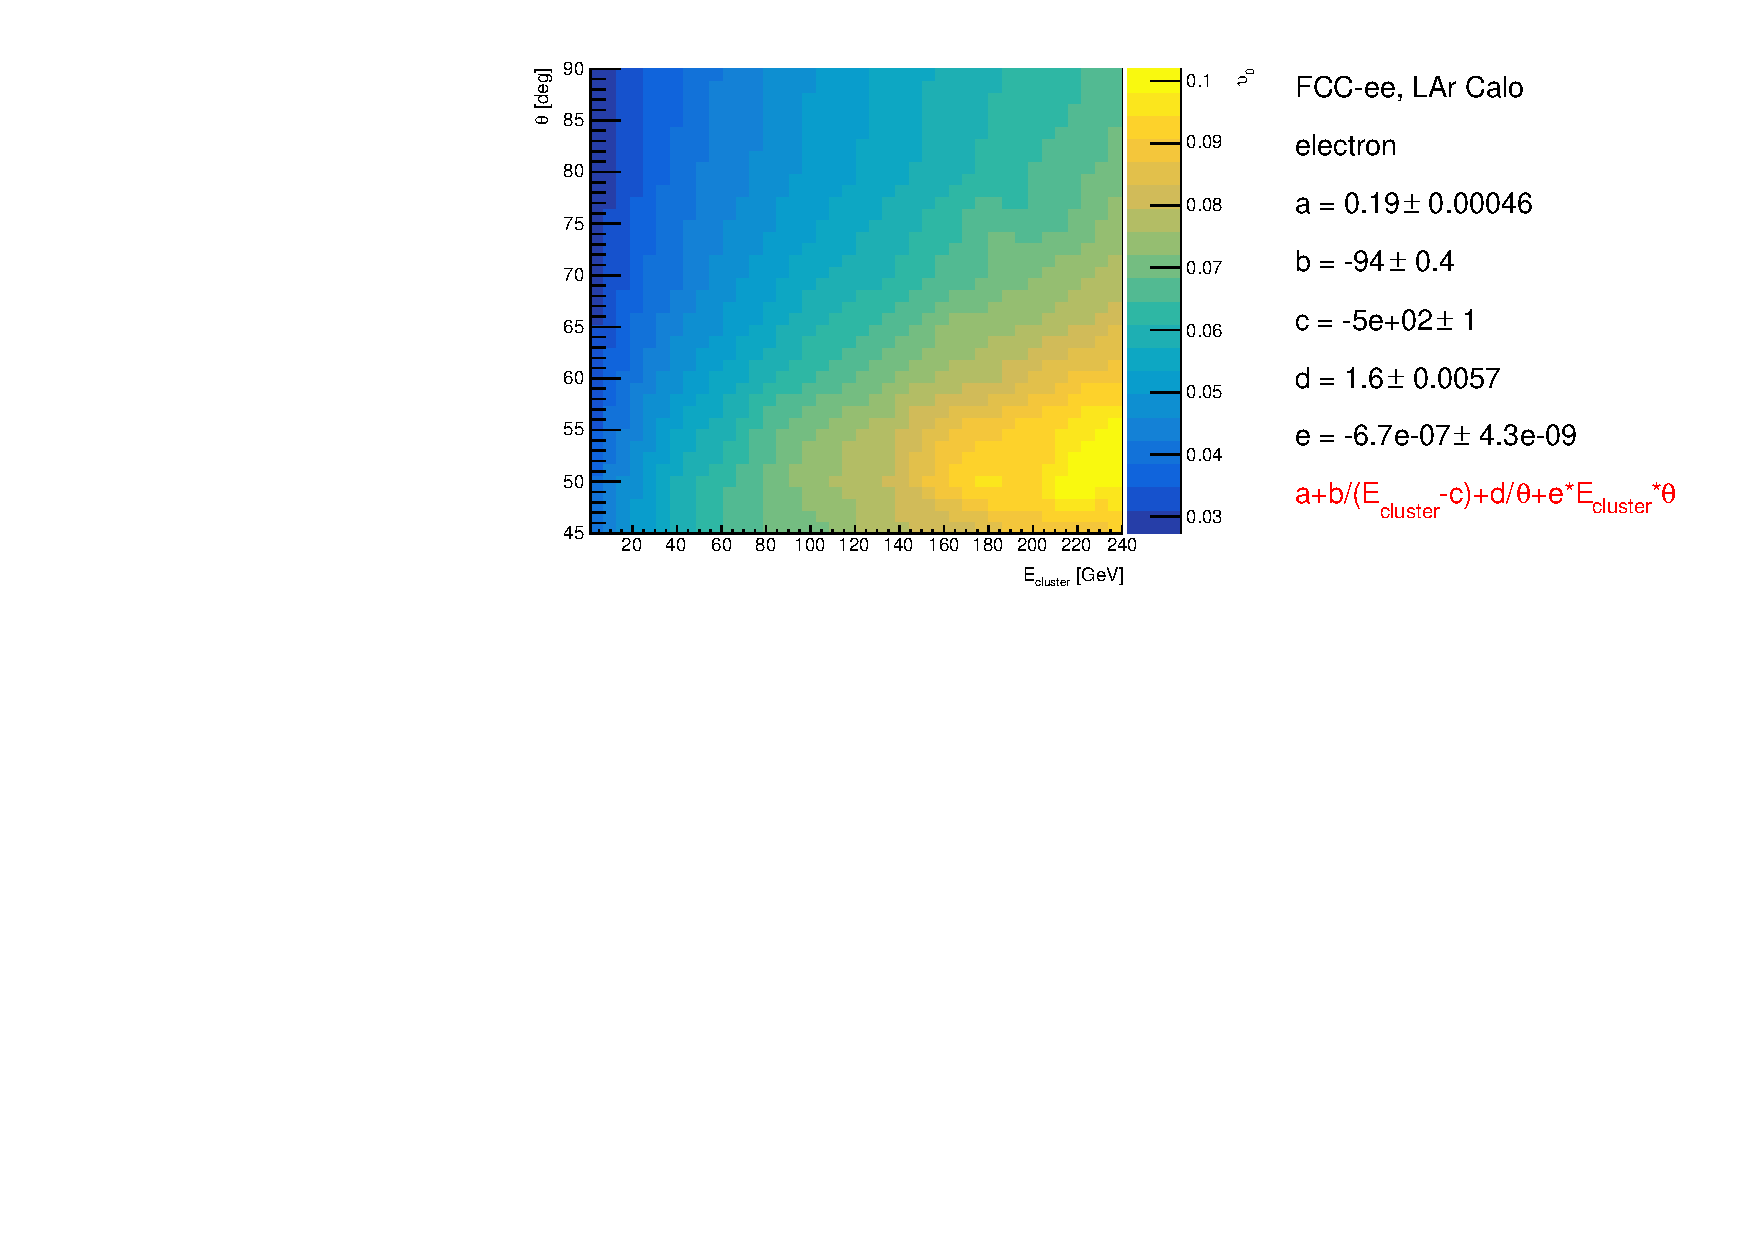
\includegraphics[width=0.49\linewidth]{figures/2d/graph_upstream_upsilon_0.pdf}
    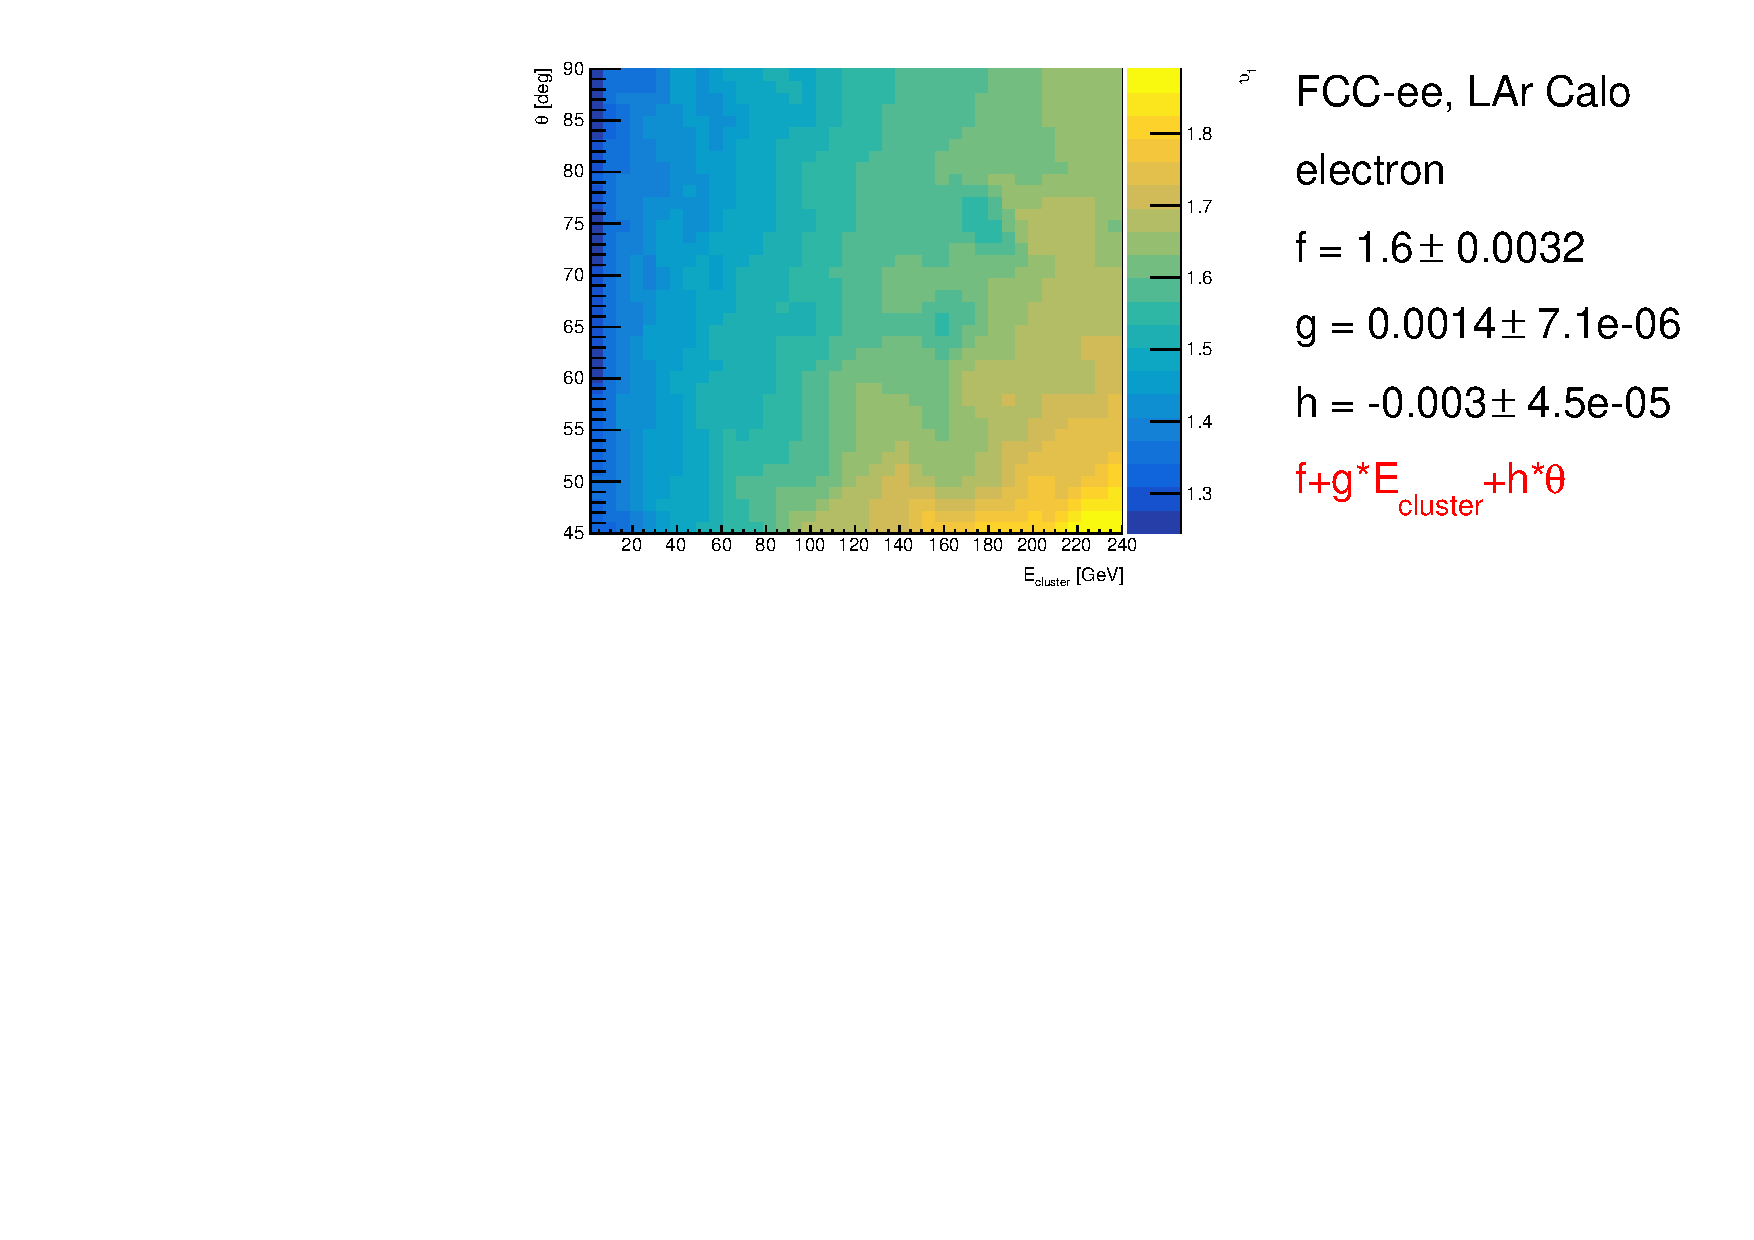
\includegraphics[width=0.49\linewidth]{figures/2d/graph_upstream_upsilon_1.pdf}
    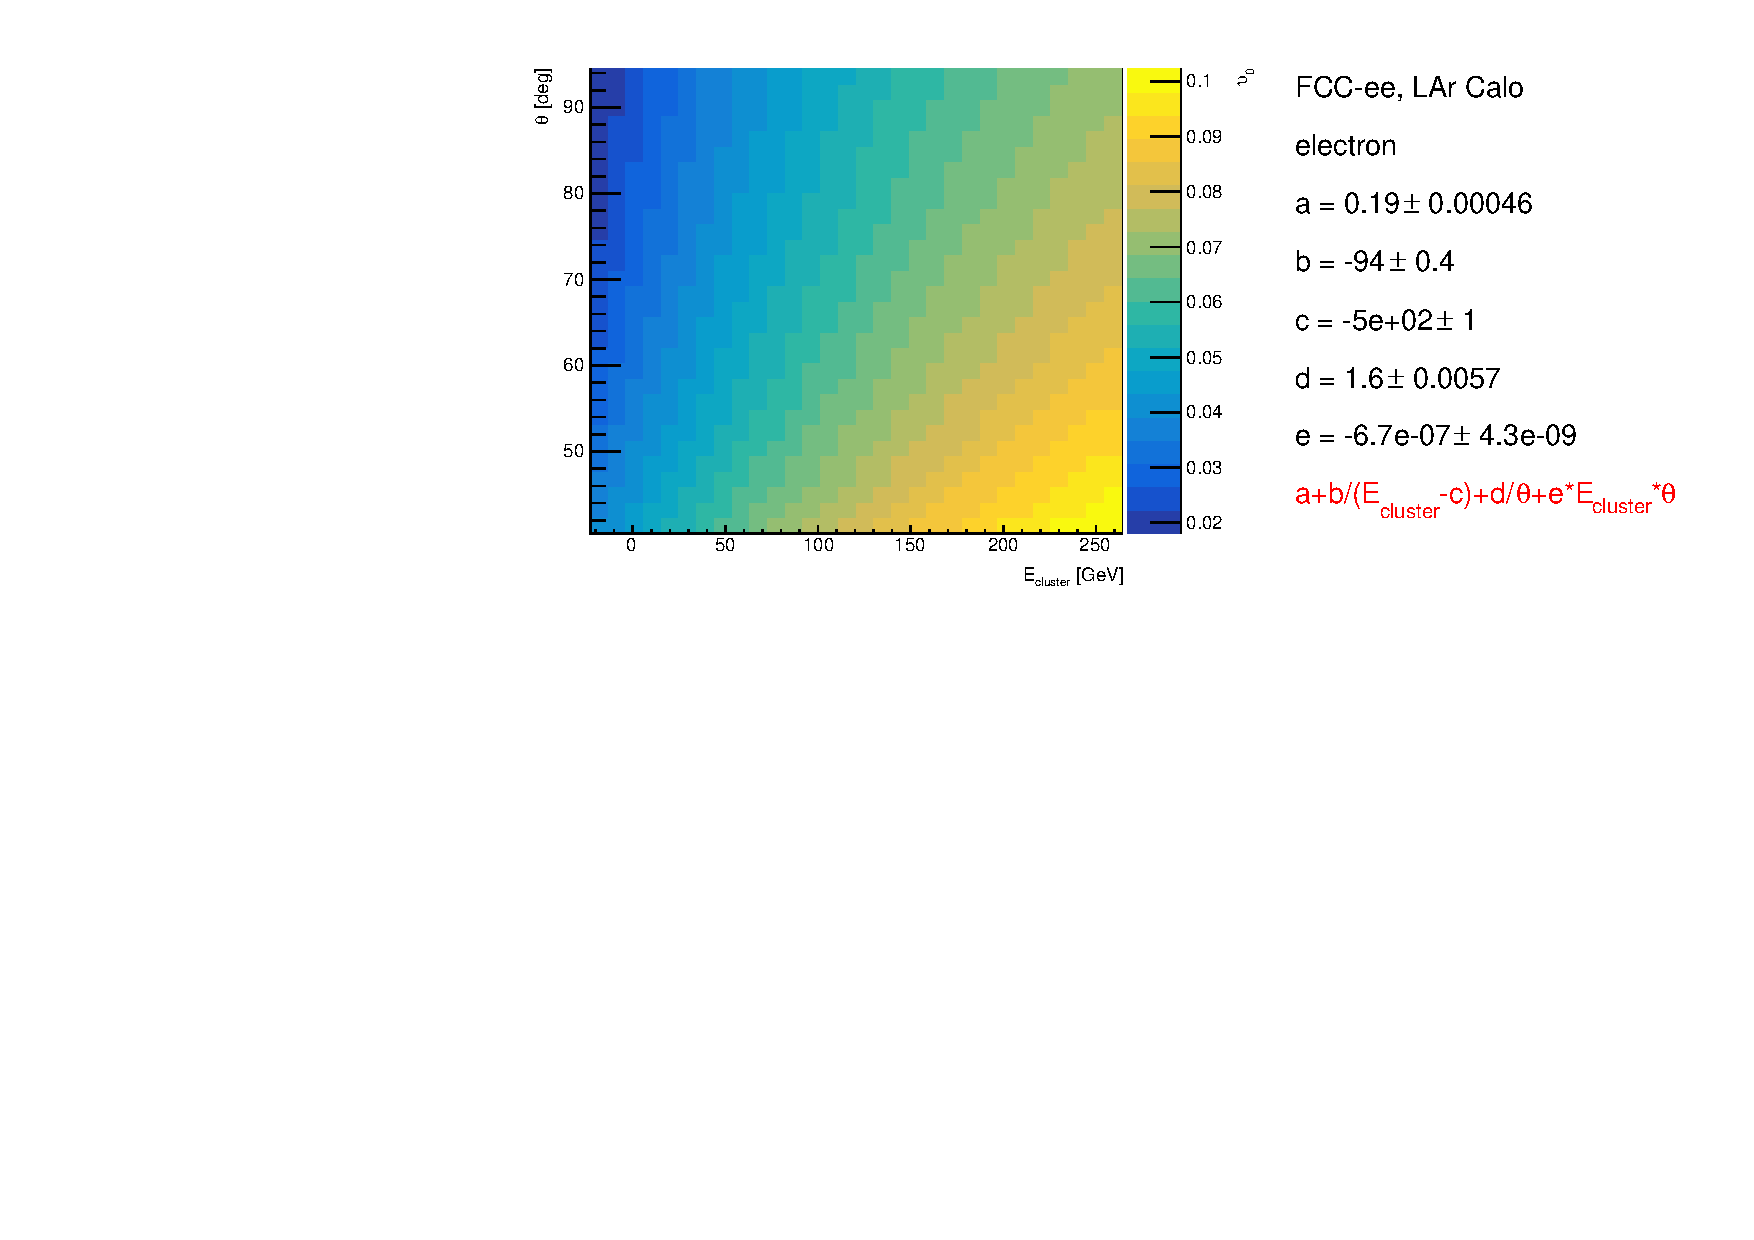
\includegraphics[width=0.49\linewidth]{figures/2d/func_upstream_upsilon_0.pdf}
    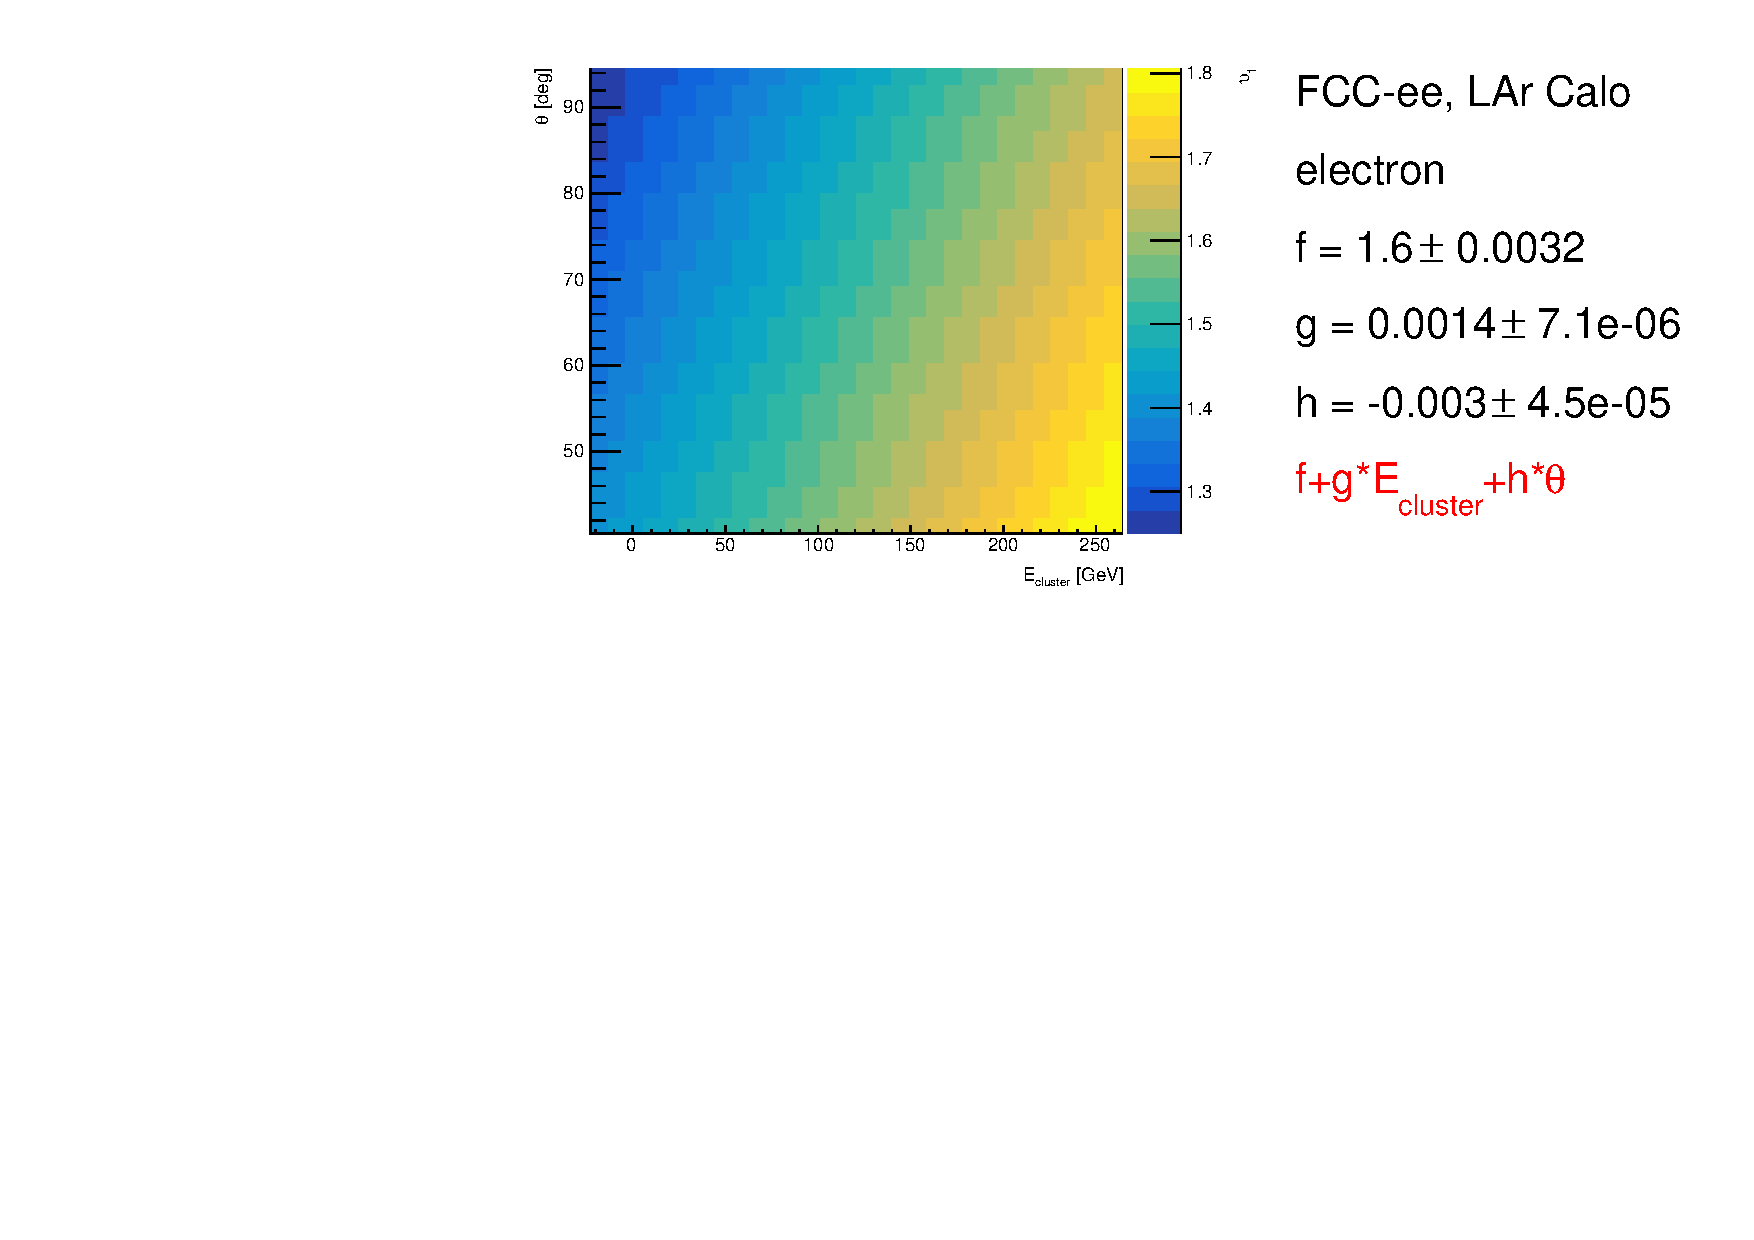
\includegraphics[width=0.49\linewidth]{figures/2d/func_upstream_upsilon_1.pdf}
  \end{adjustwidth}
\end{frame}

\begin{frame}
  \frametitle{FCC-ee Downstream Correction Energy Dependence}

  \begin{adjustwidth}{-9mm}{-9mm}
    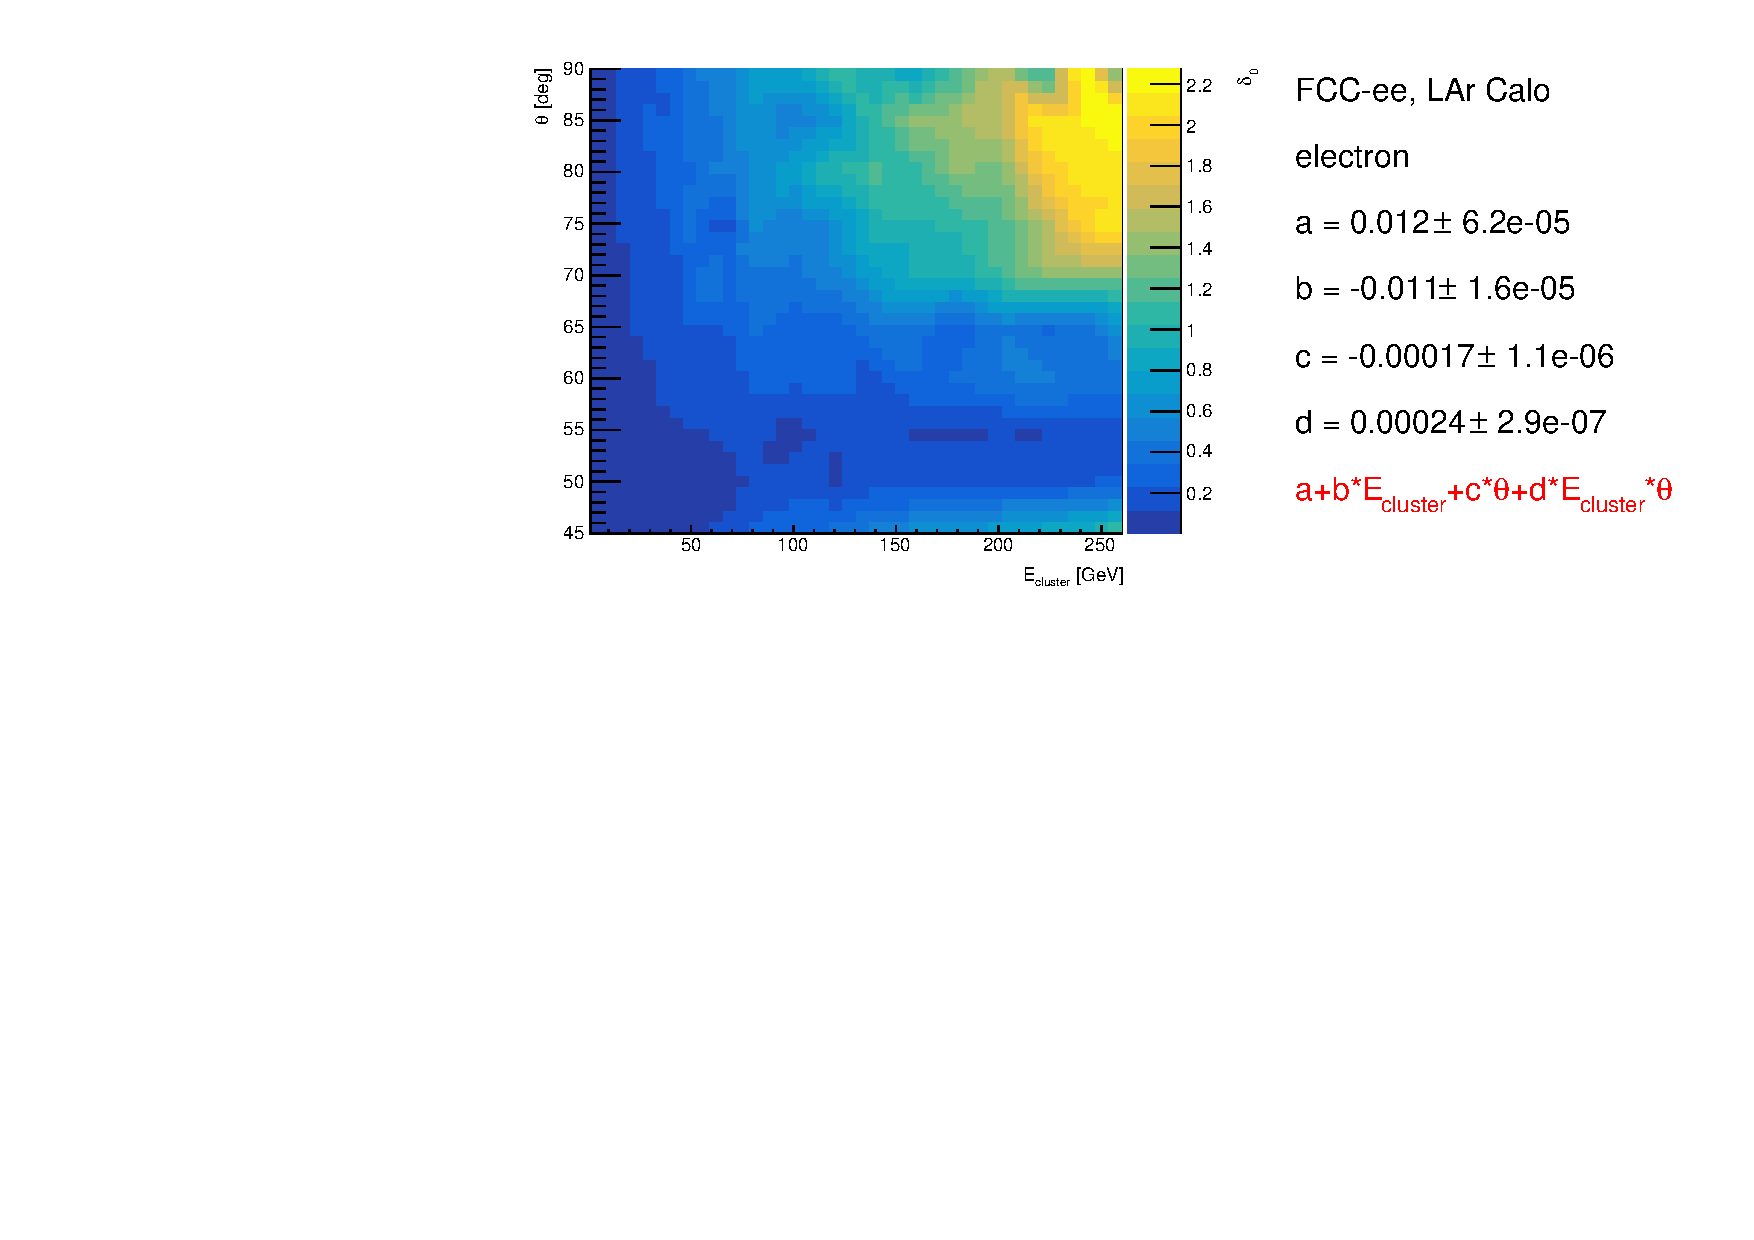
\includegraphics[width=0.32\linewidth]{figures/2d/graph_downstream_delta_0.pdf}
    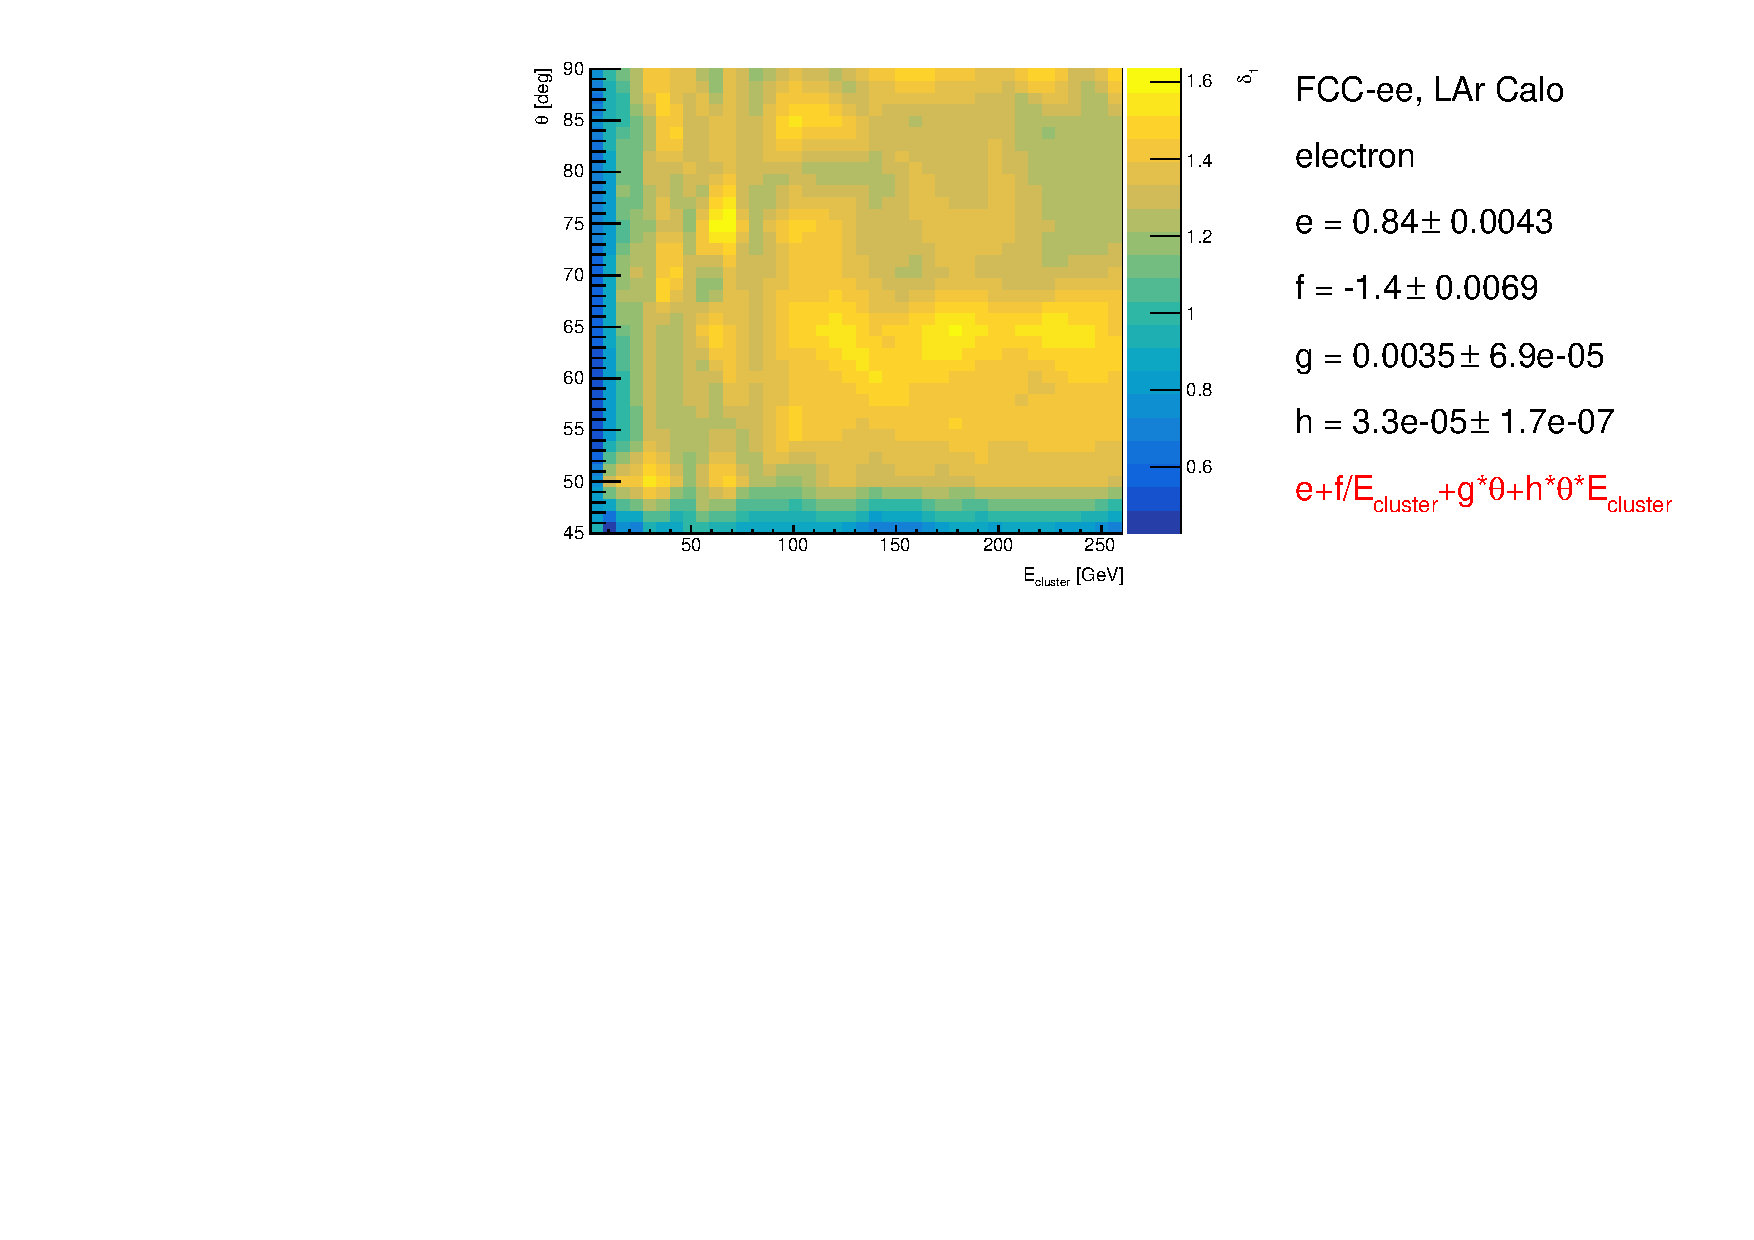
\includegraphics[width=0.32\linewidth]{figures/2d/graph_downstream_delta_1.pdf}
    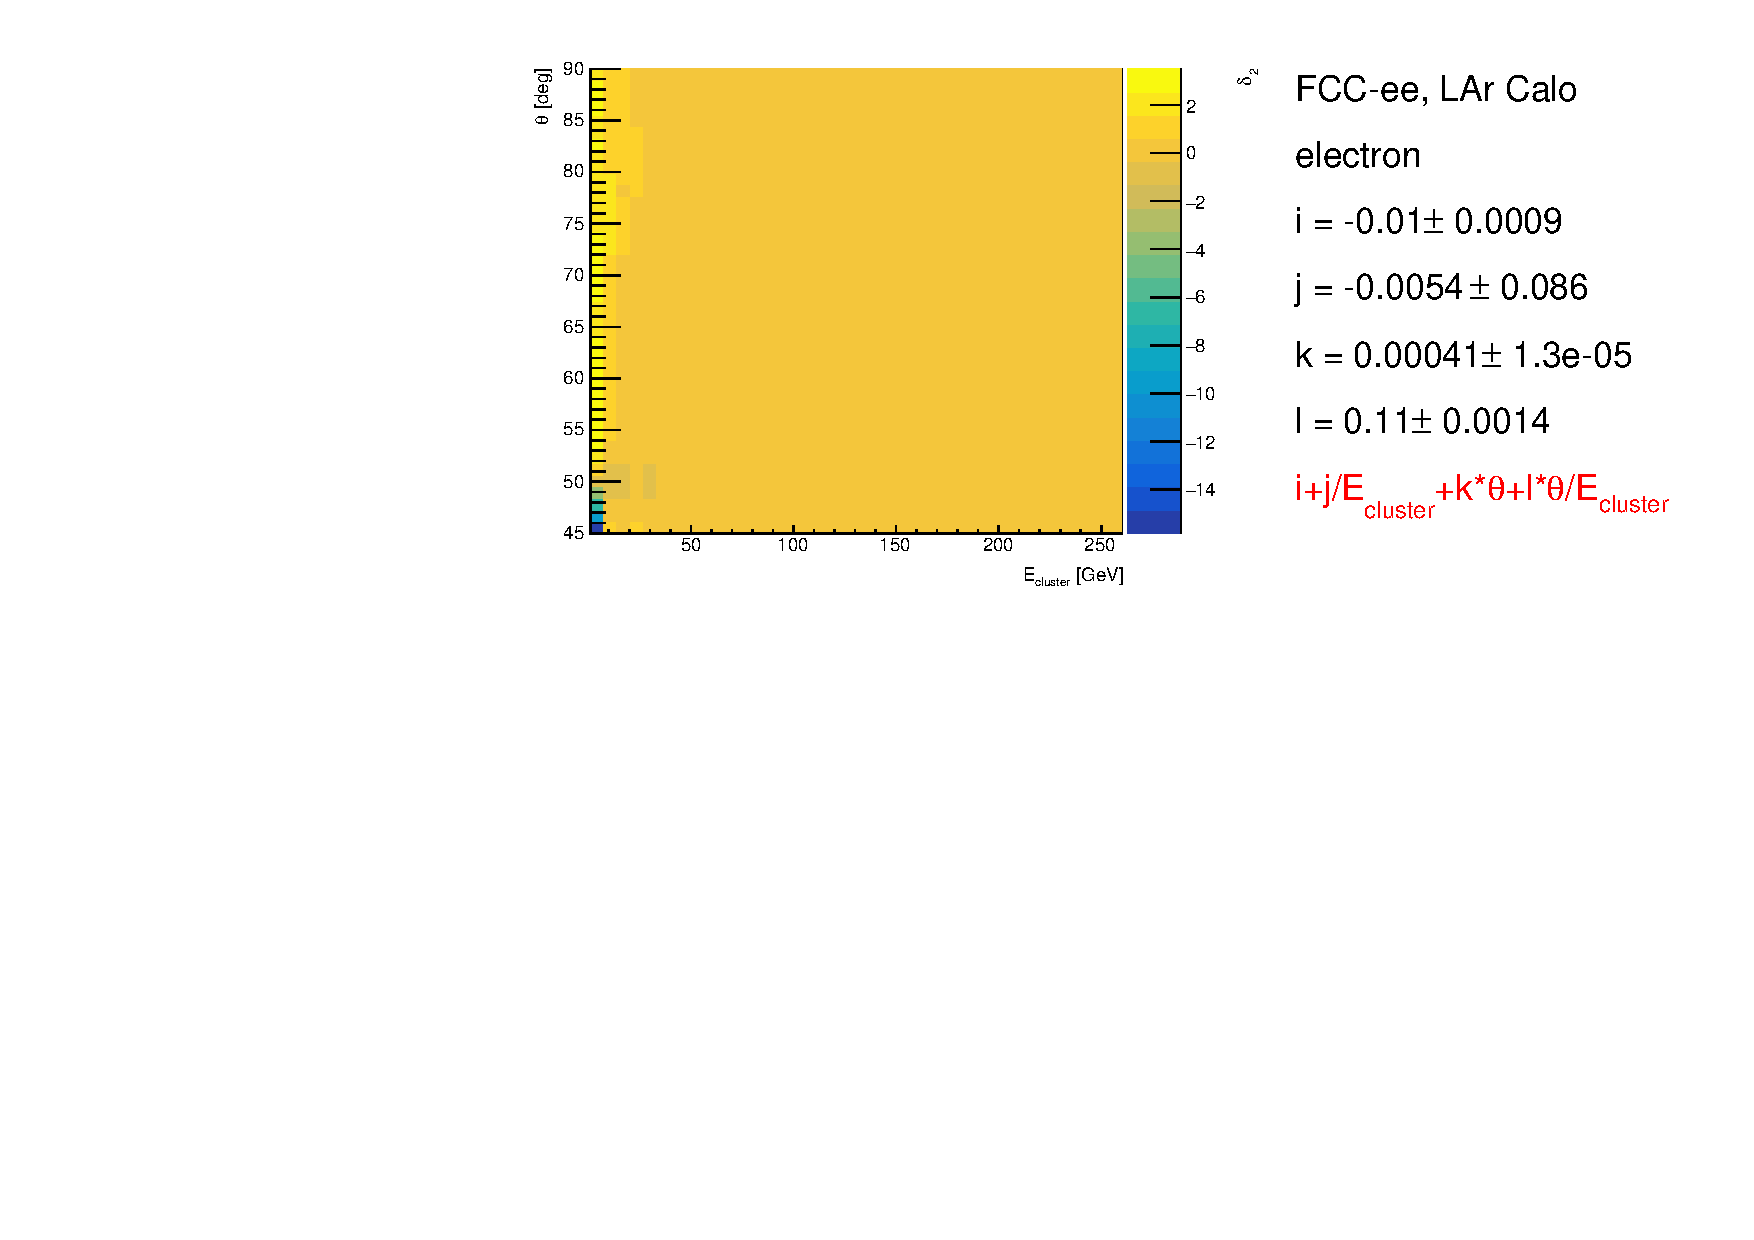
\includegraphics[width=0.32\linewidth]{figures/2d/graph_downstream_delta_2.pdf}
    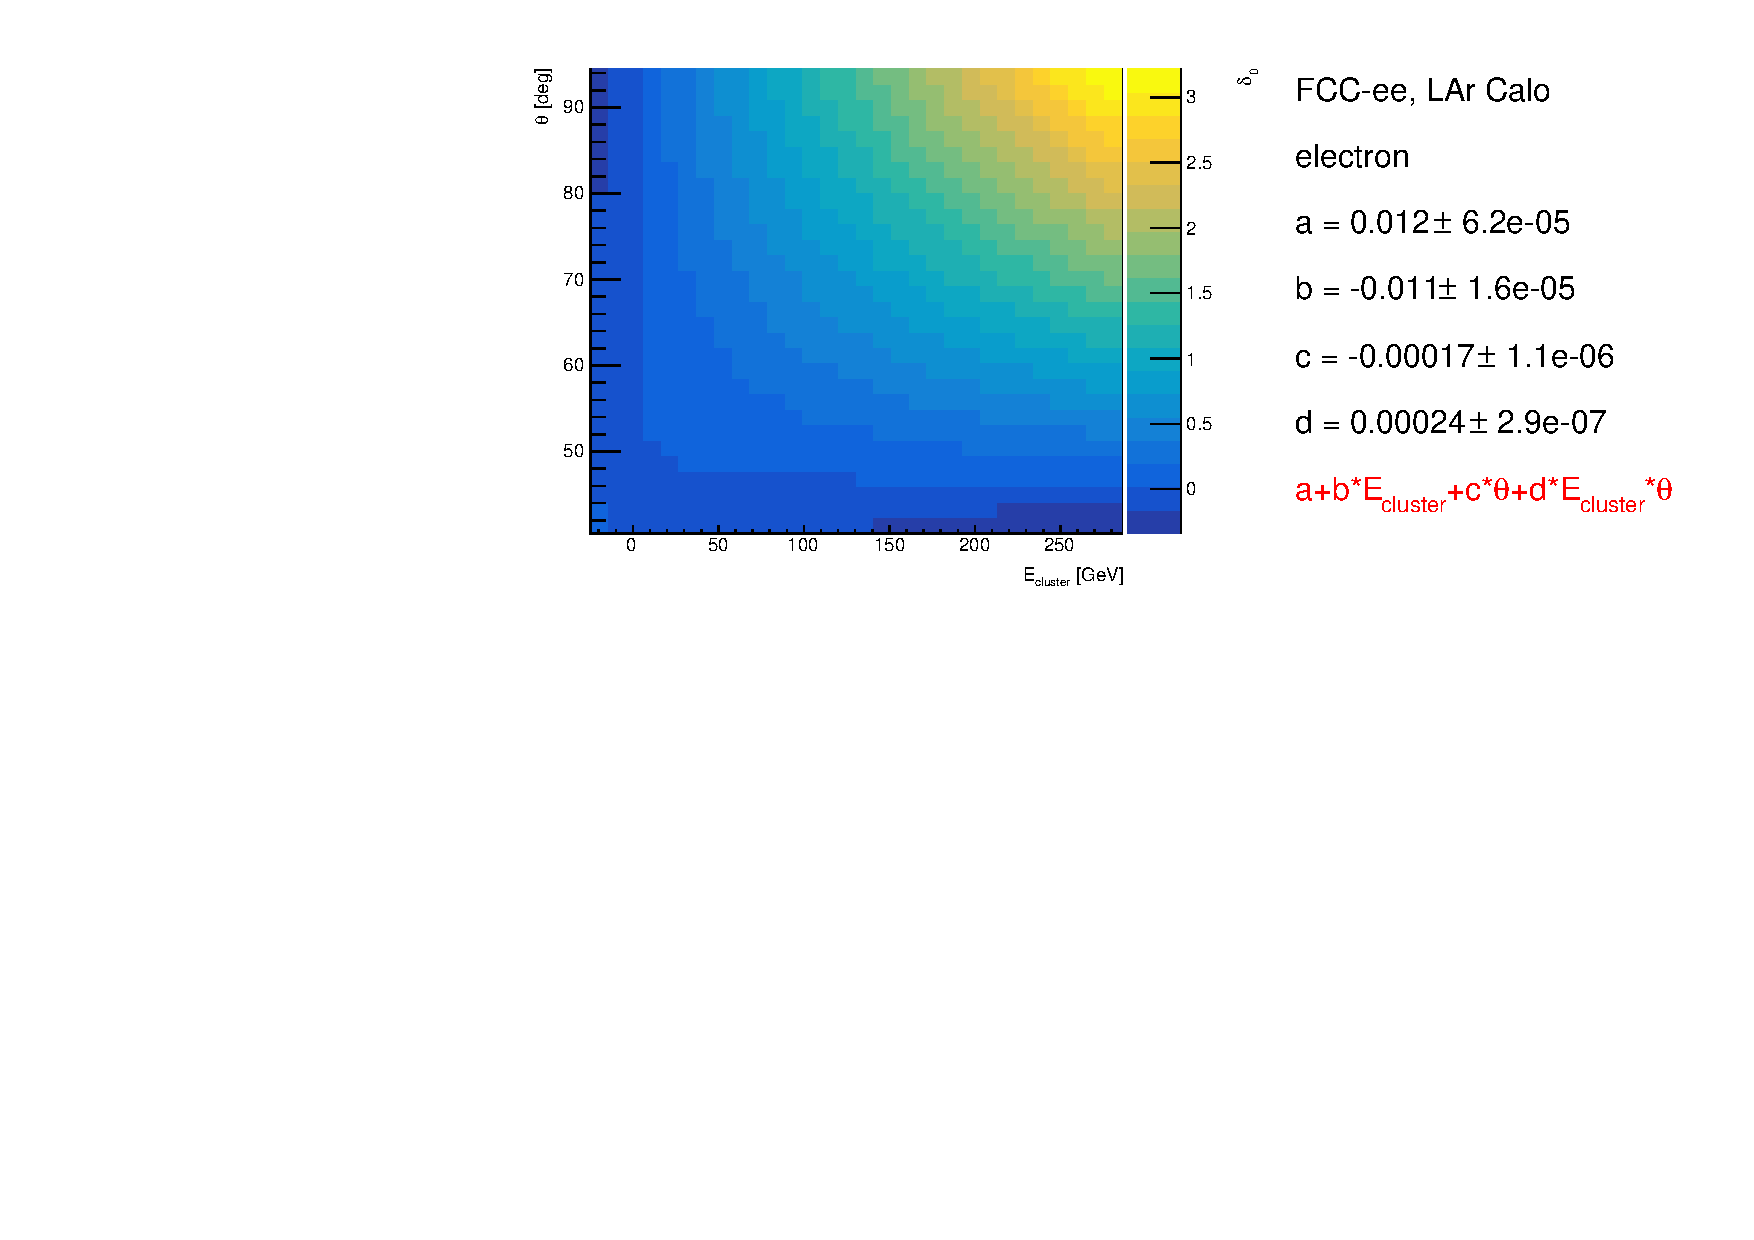
\includegraphics[width=0.32\linewidth]{figures/2d/func_downstream_delta_0.pdf}
    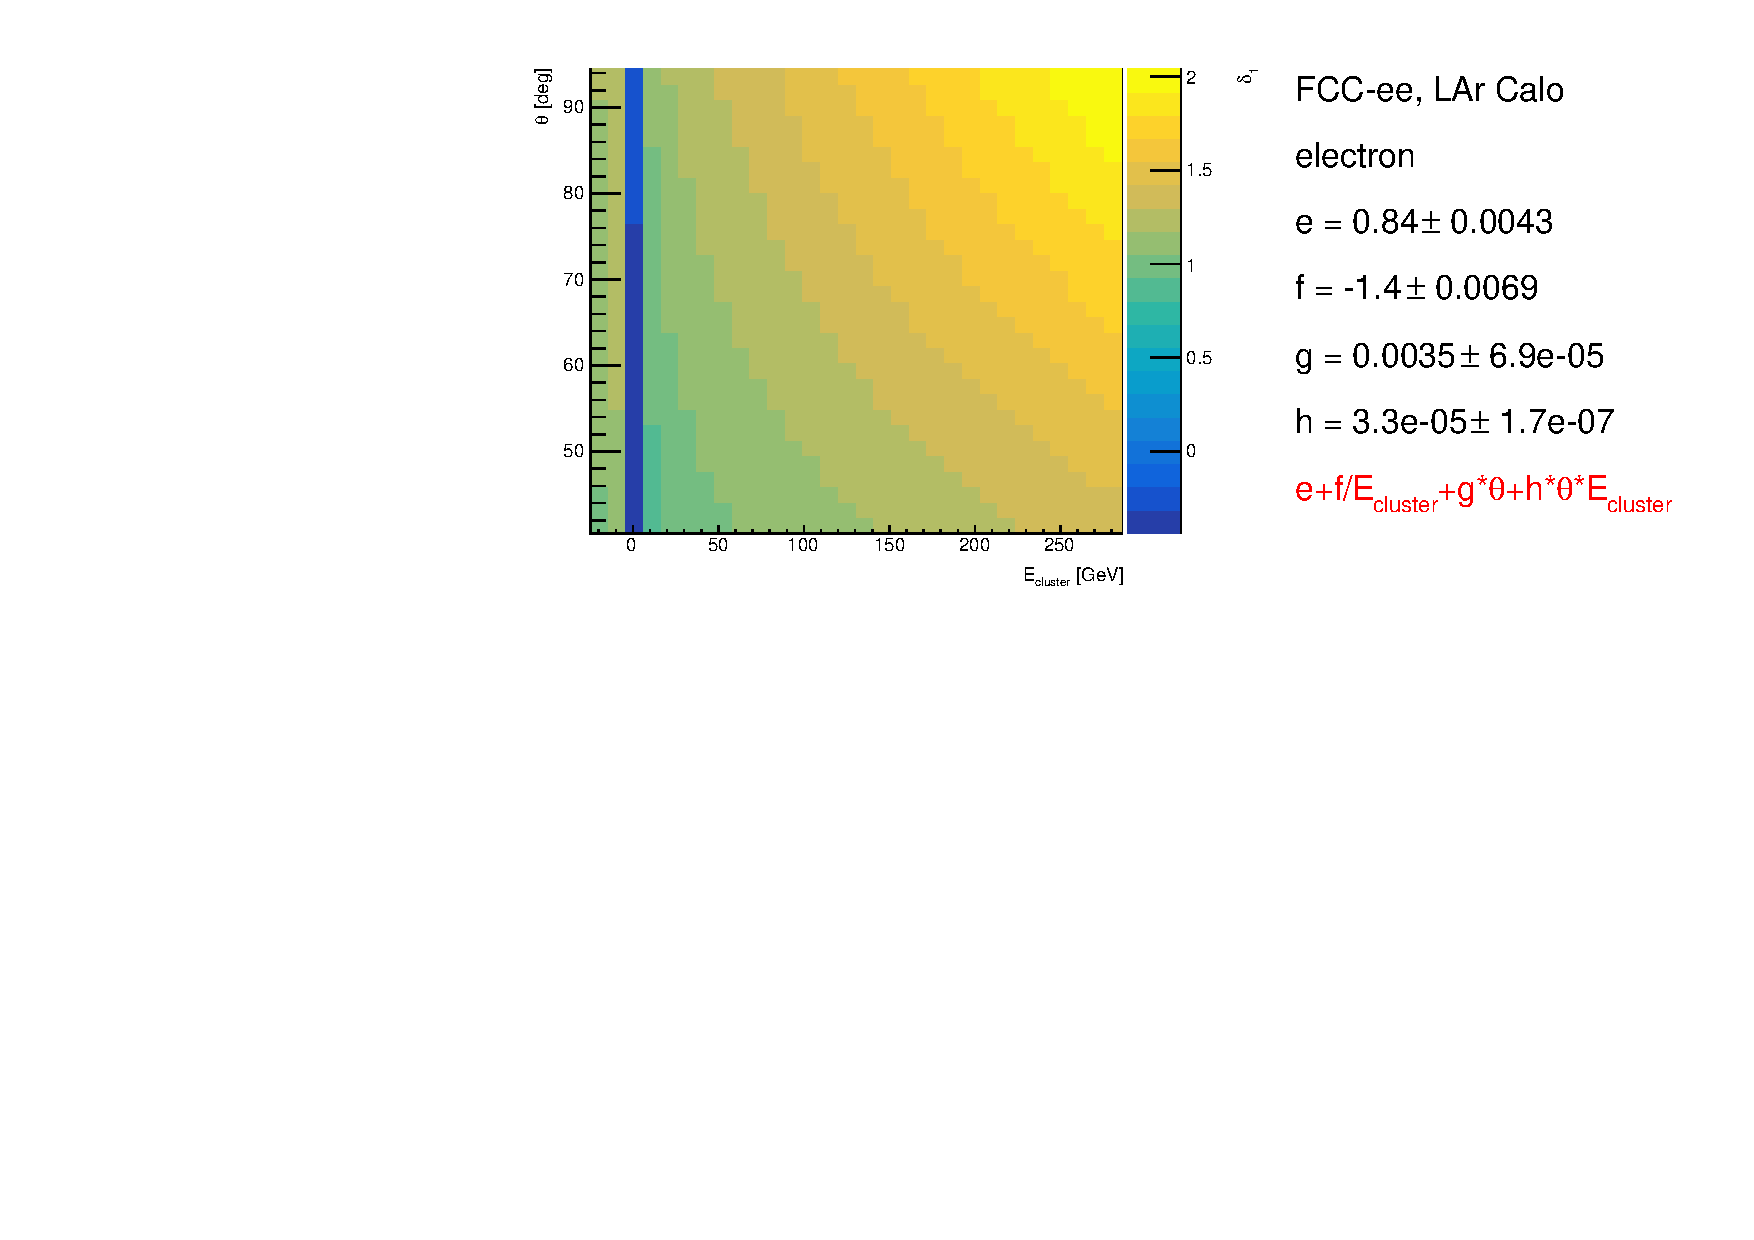
\includegraphics[width=0.32\linewidth]{figures/2d/func_downstream_delta_1.pdf}
    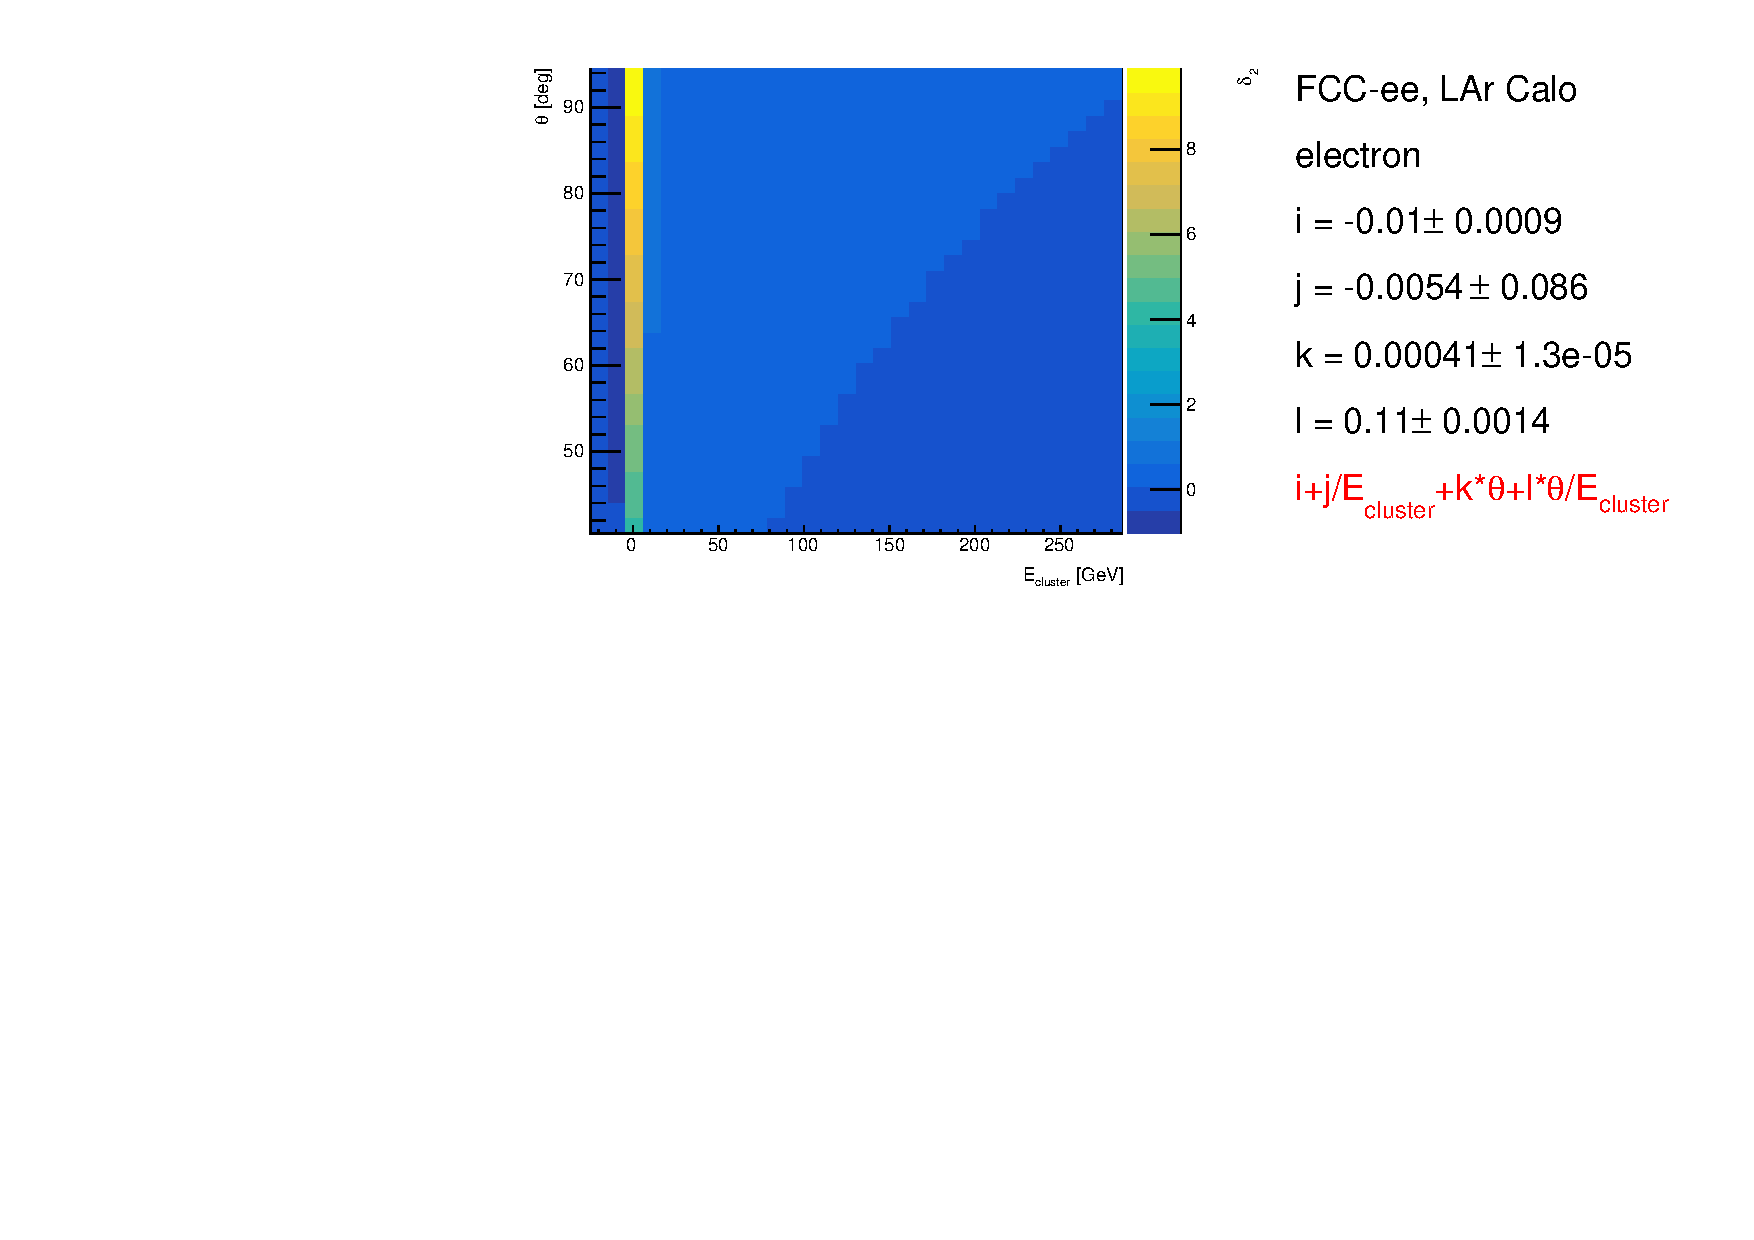
\includegraphics[width=0.32\linewidth]{figures/2d/func_downstream_delta_2.pdf}
  \end{adjustwidth}
\end{frame}


% ---------------------------------------------------------------------------- %
\section{Energy correction test}

\begin{frame}
  \frametitle{FCC-ee: Energy correction test I.}

  \centering
  FCC-ee, $e^{-}$, \redtext{10 GeV}, $\theta = 70$ deg \hspace{8mm}
  FCC-ee, $e^{-}$, \redtext{30 GeV}, $\theta = 70$ deg \\[1.5ex]
  \begin{adjustwidth}{-5mm}{-5mm}
    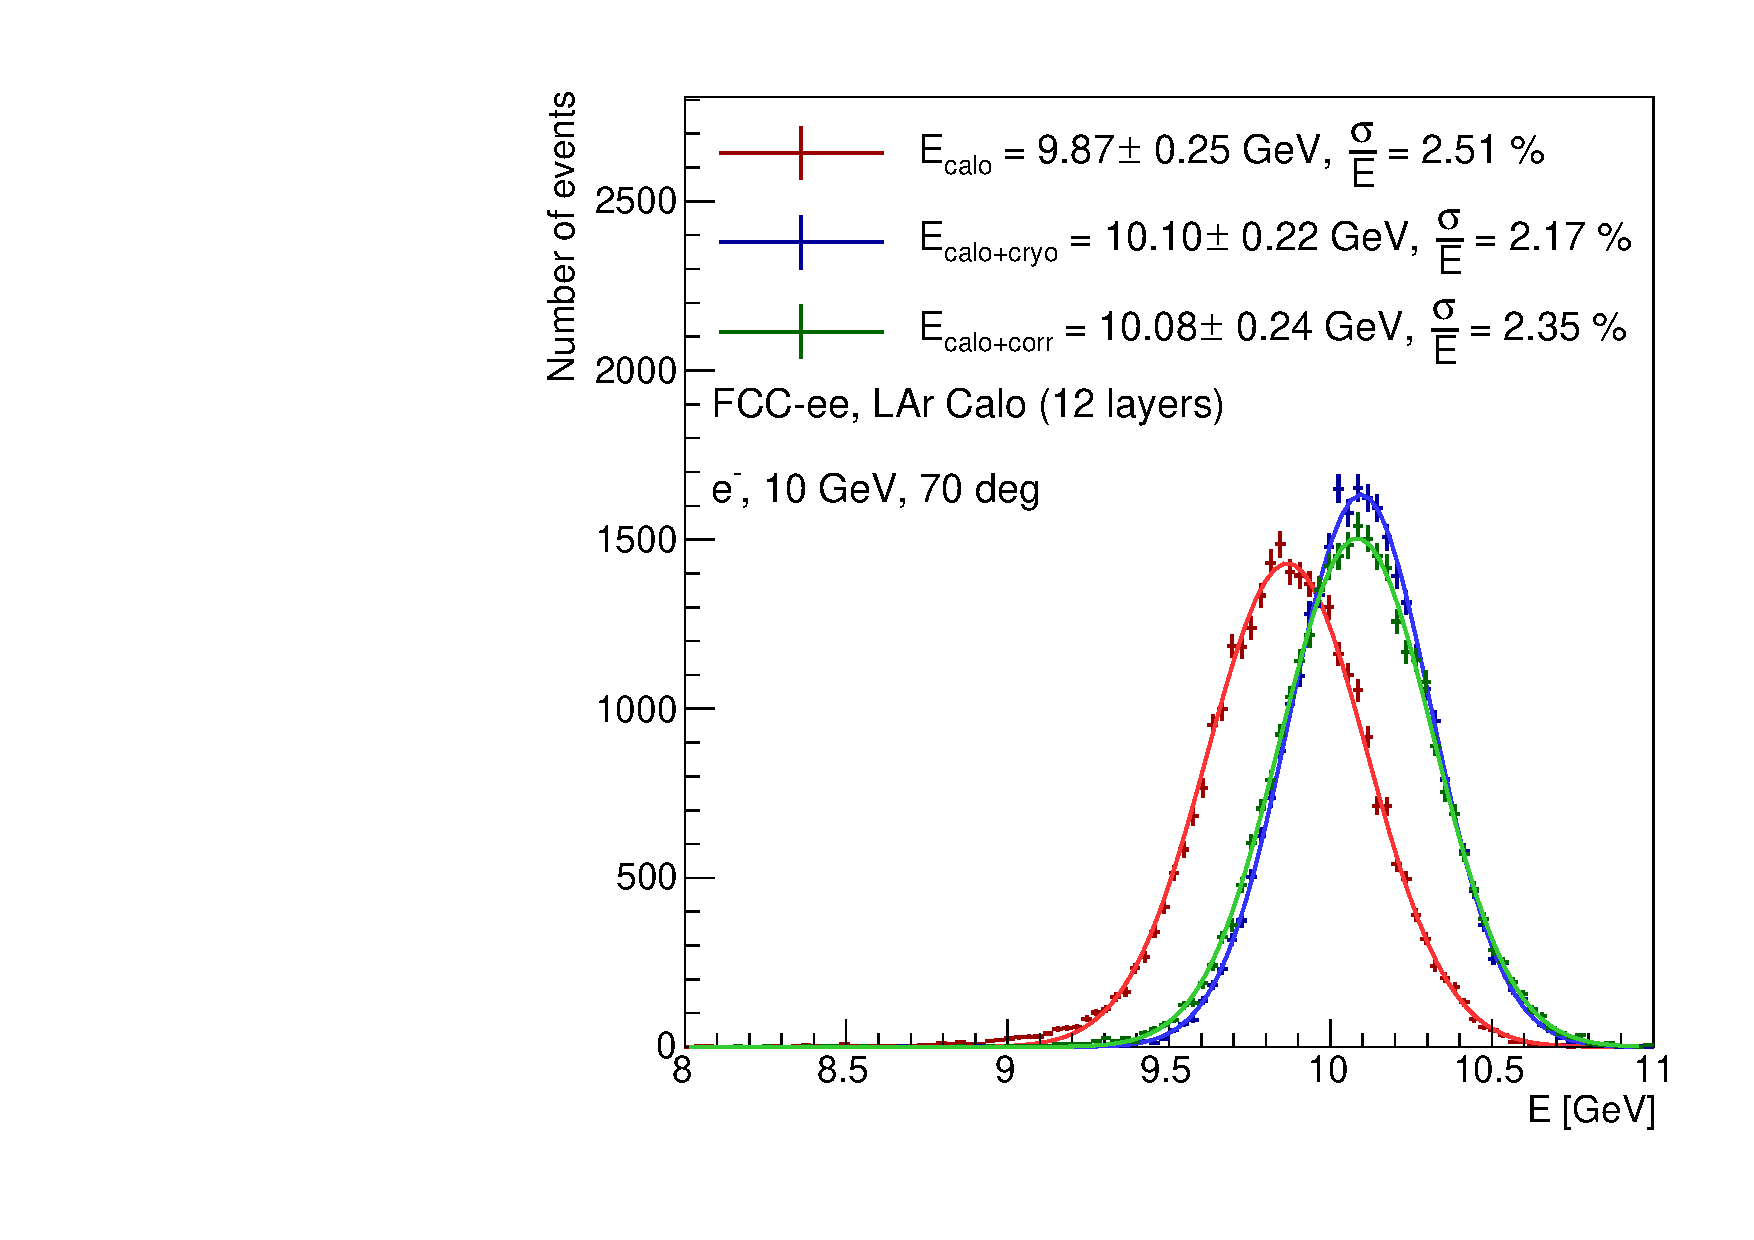
\includegraphics[width=0.49\linewidth]{figures/2d/hist_energy_corr_test_70deg_10GeV.pdf}
    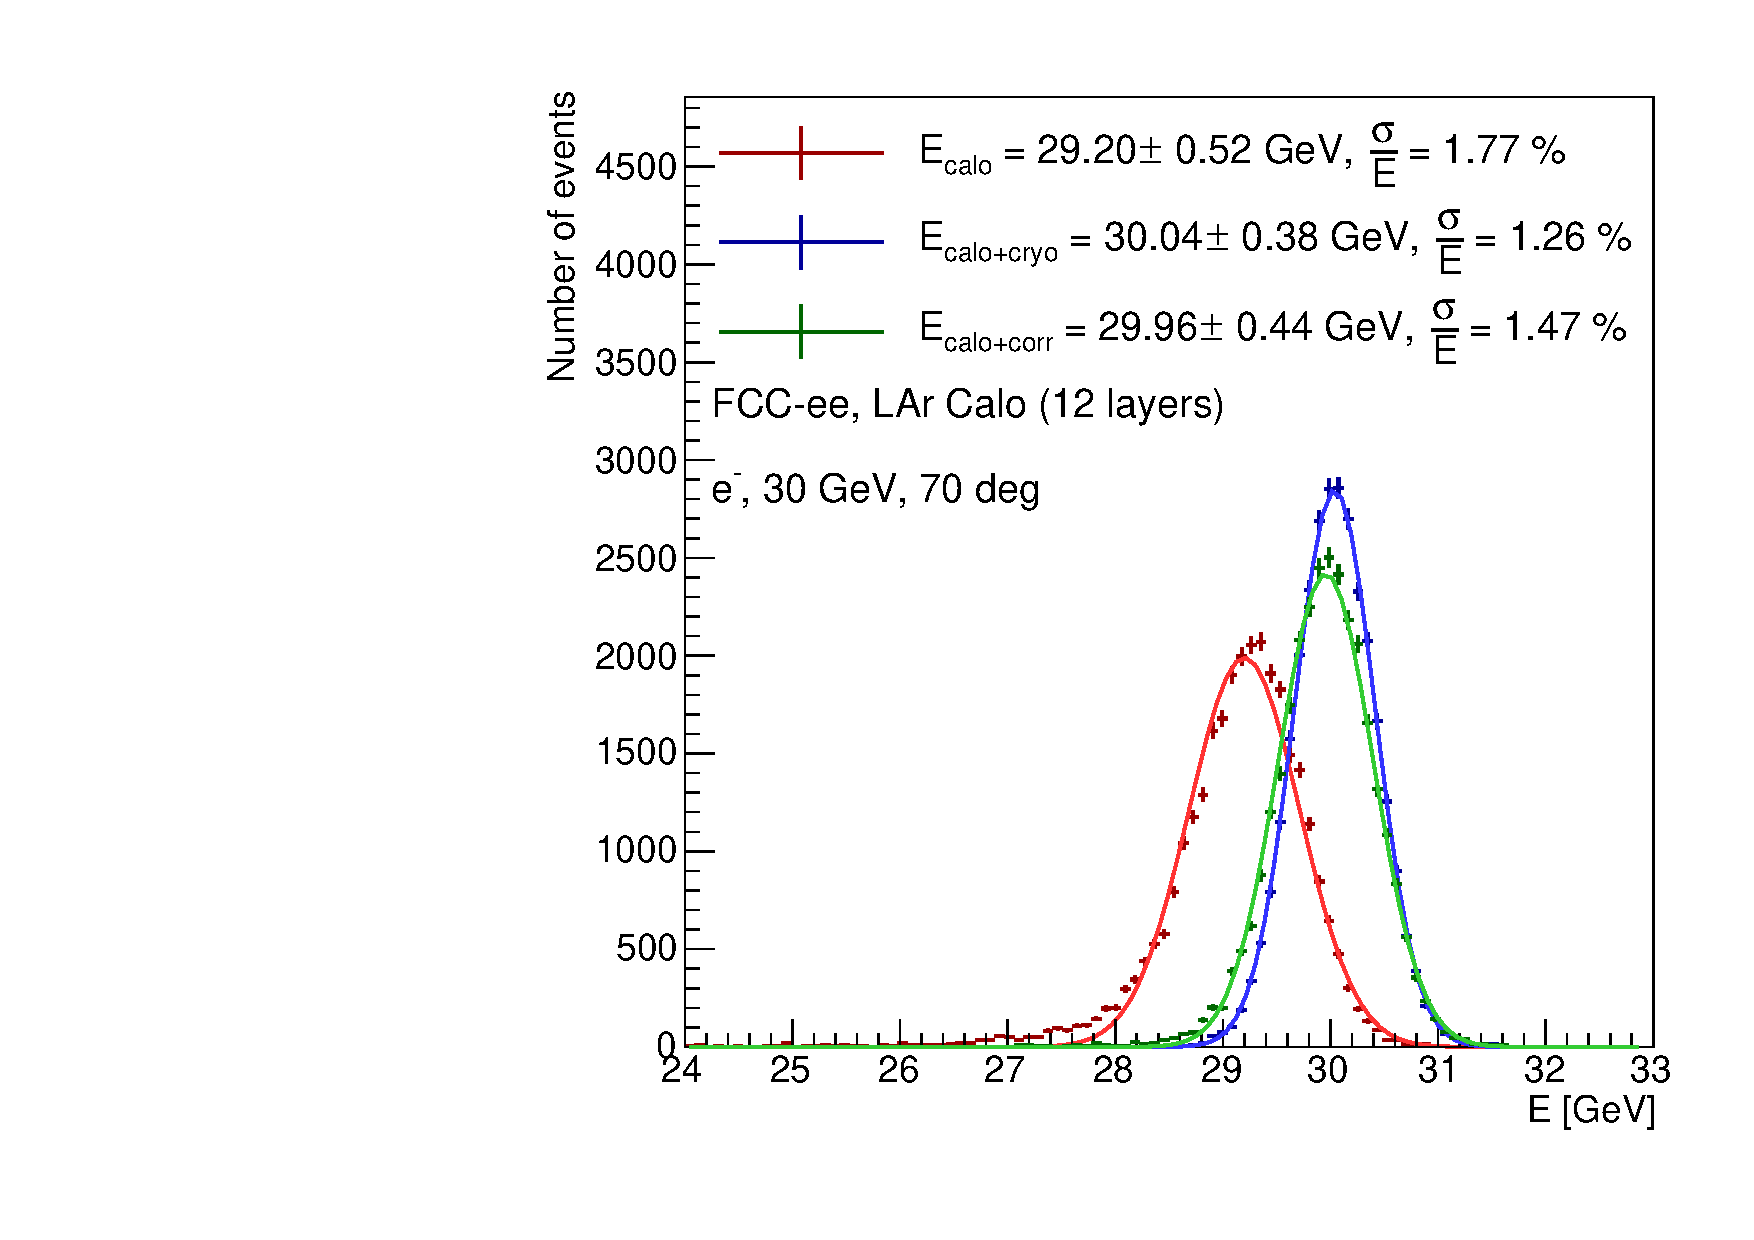
\includegraphics[width=0.49\linewidth]{figures/2d/hist_energy_corr_test_70deg_30GeV.pdf}
  \end{adjustwidth}
\end{frame}

\begin{frame}
  \frametitle{FCC-ee: Energy correction test II.}

  \centering
  FCC-ee, $e^{-}$, \redtext{50 GeV}, $\theta = 70$ deg \hspace{8mm}
  FCC-ee, $e^{-}$, \redtext{80 GeV}, $\theta = 70$ deg \\[1.5ex]
  \begin{adjustwidth}{-5mm}{-5mm}
    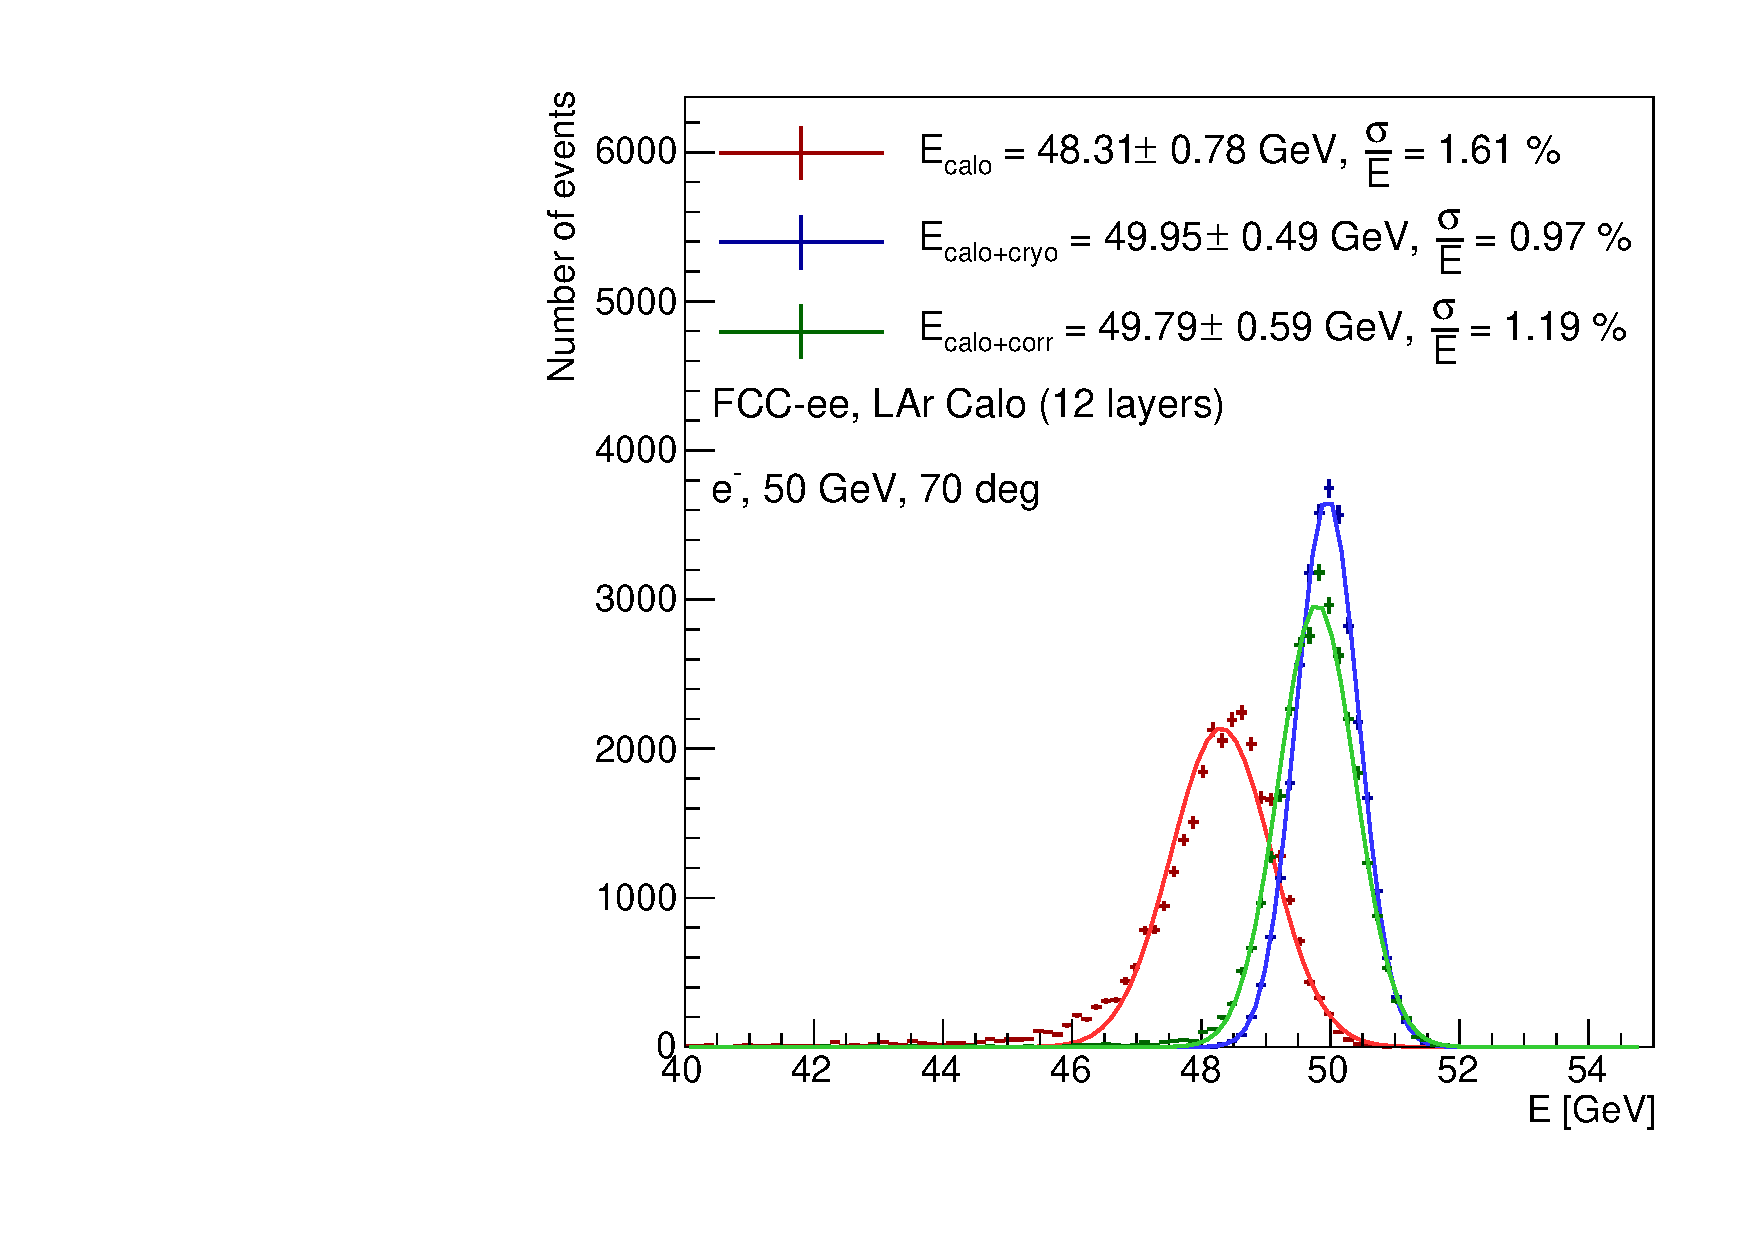
\includegraphics[width=0.49\linewidth]{figures/2d/hist_energy_corr_test_70deg_50GeV.pdf}
    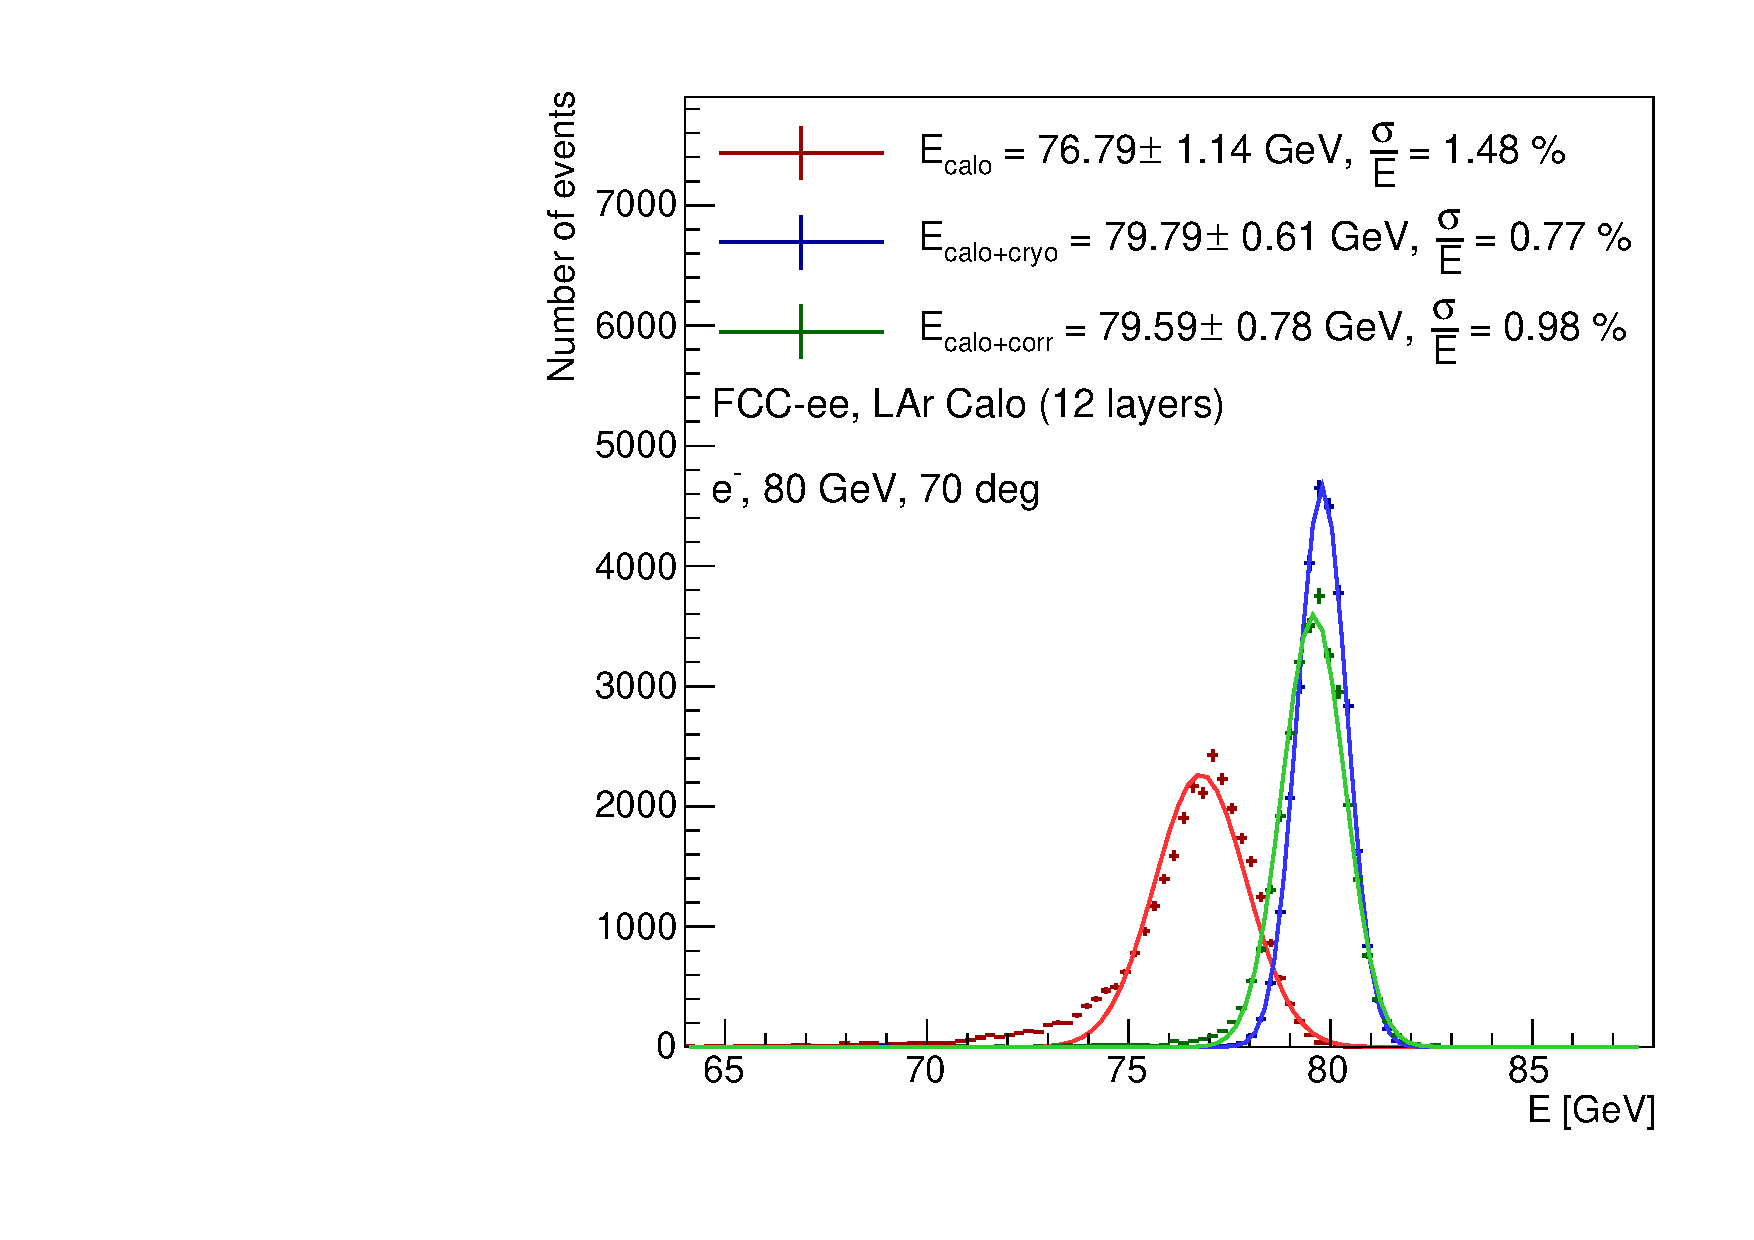
\includegraphics[width=0.49\linewidth]{figures/2d/hist_energy_corr_test_70deg_80GeV.pdf}
  \end{adjustwidth}
\end{frame}

\begin{frame}
  \frametitle{FCC-ee: Energy correction test III.}

  \centering
  FCC-ee, $e^{-}$, \redtext{120 GeV}, $\theta = 70$ deg \hspace{5mm}
  FCC-ee, $e^{-}$, \redtext{180 GeV}, $\theta = 70$ deg \\[1.5ex]
  \begin{adjustwidth}{-5mm}{-5mm}
    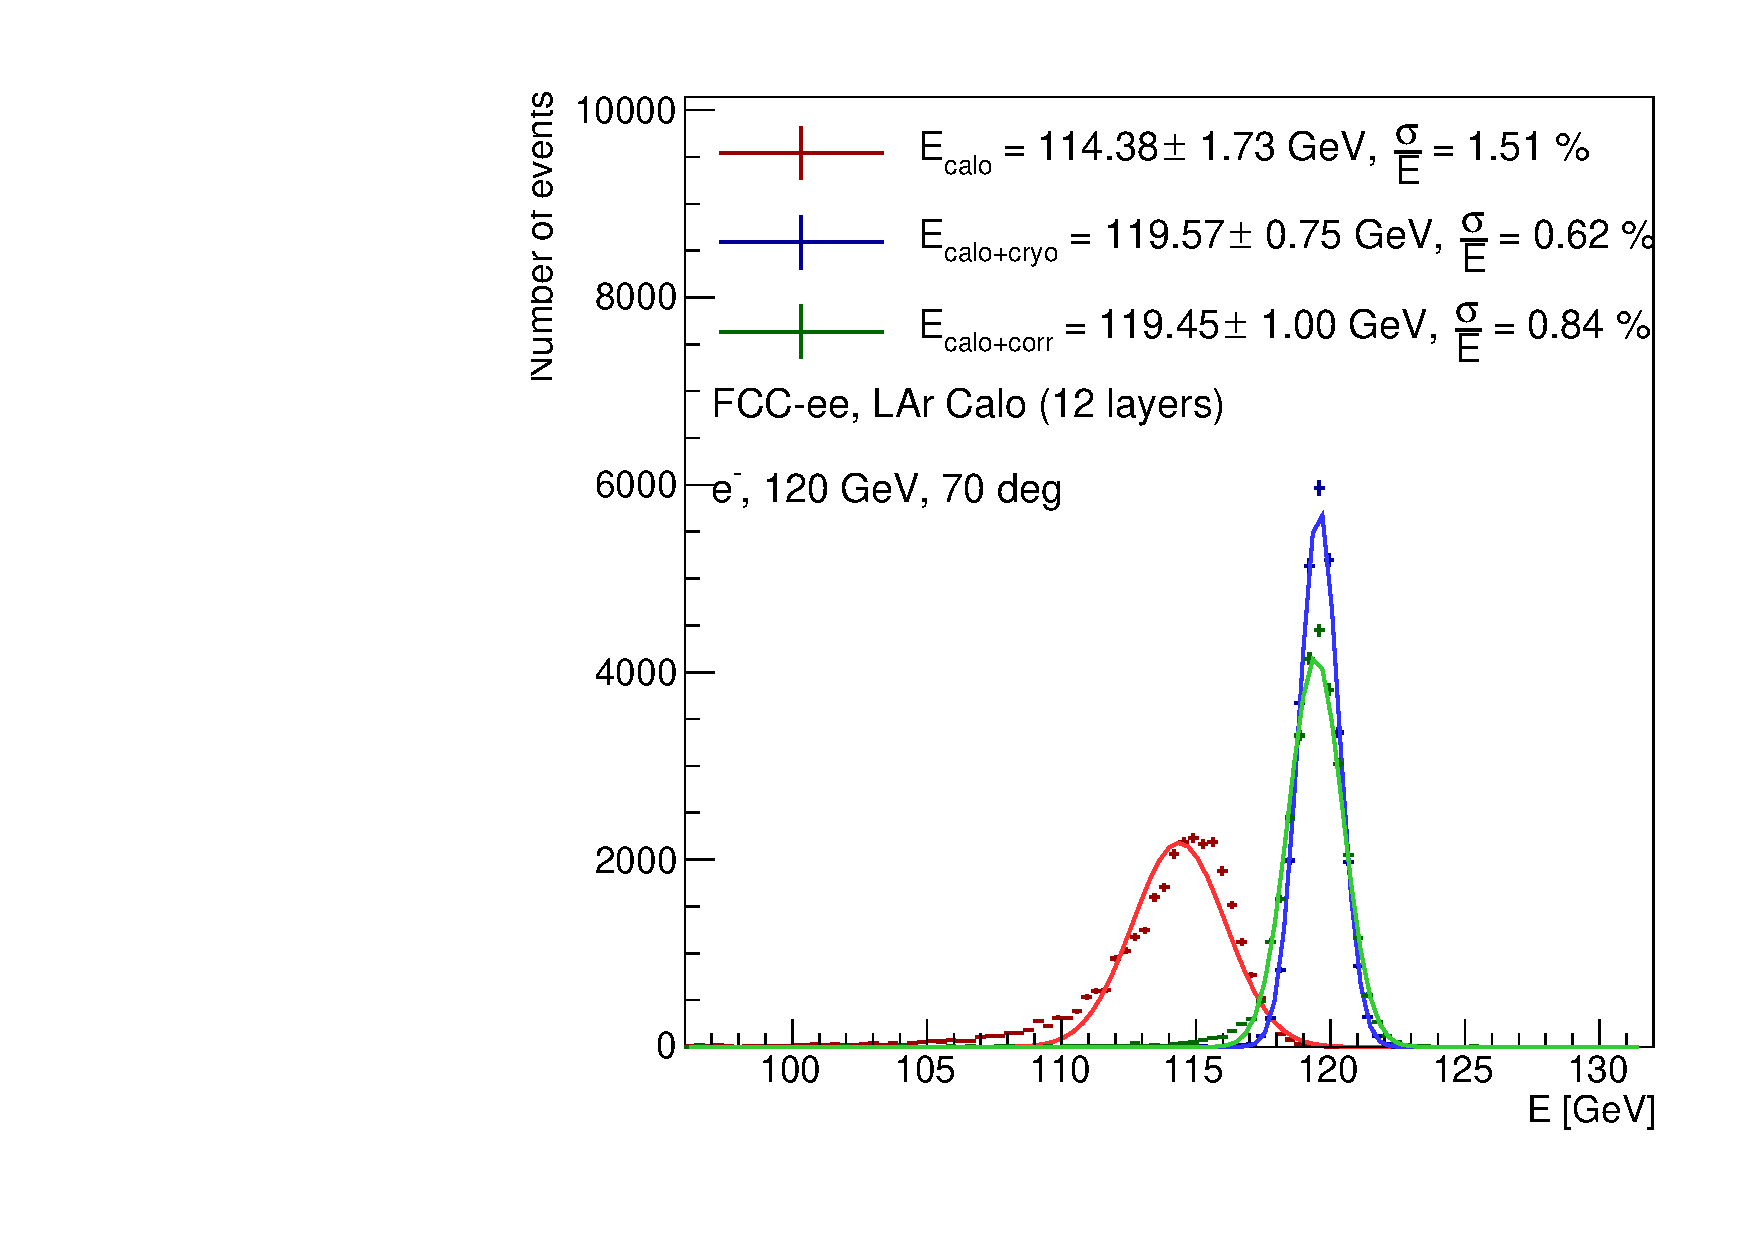
\includegraphics[width=0.49\linewidth]{figures/2d/hist_energy_corr_test_70deg_120GeV.pdf}
    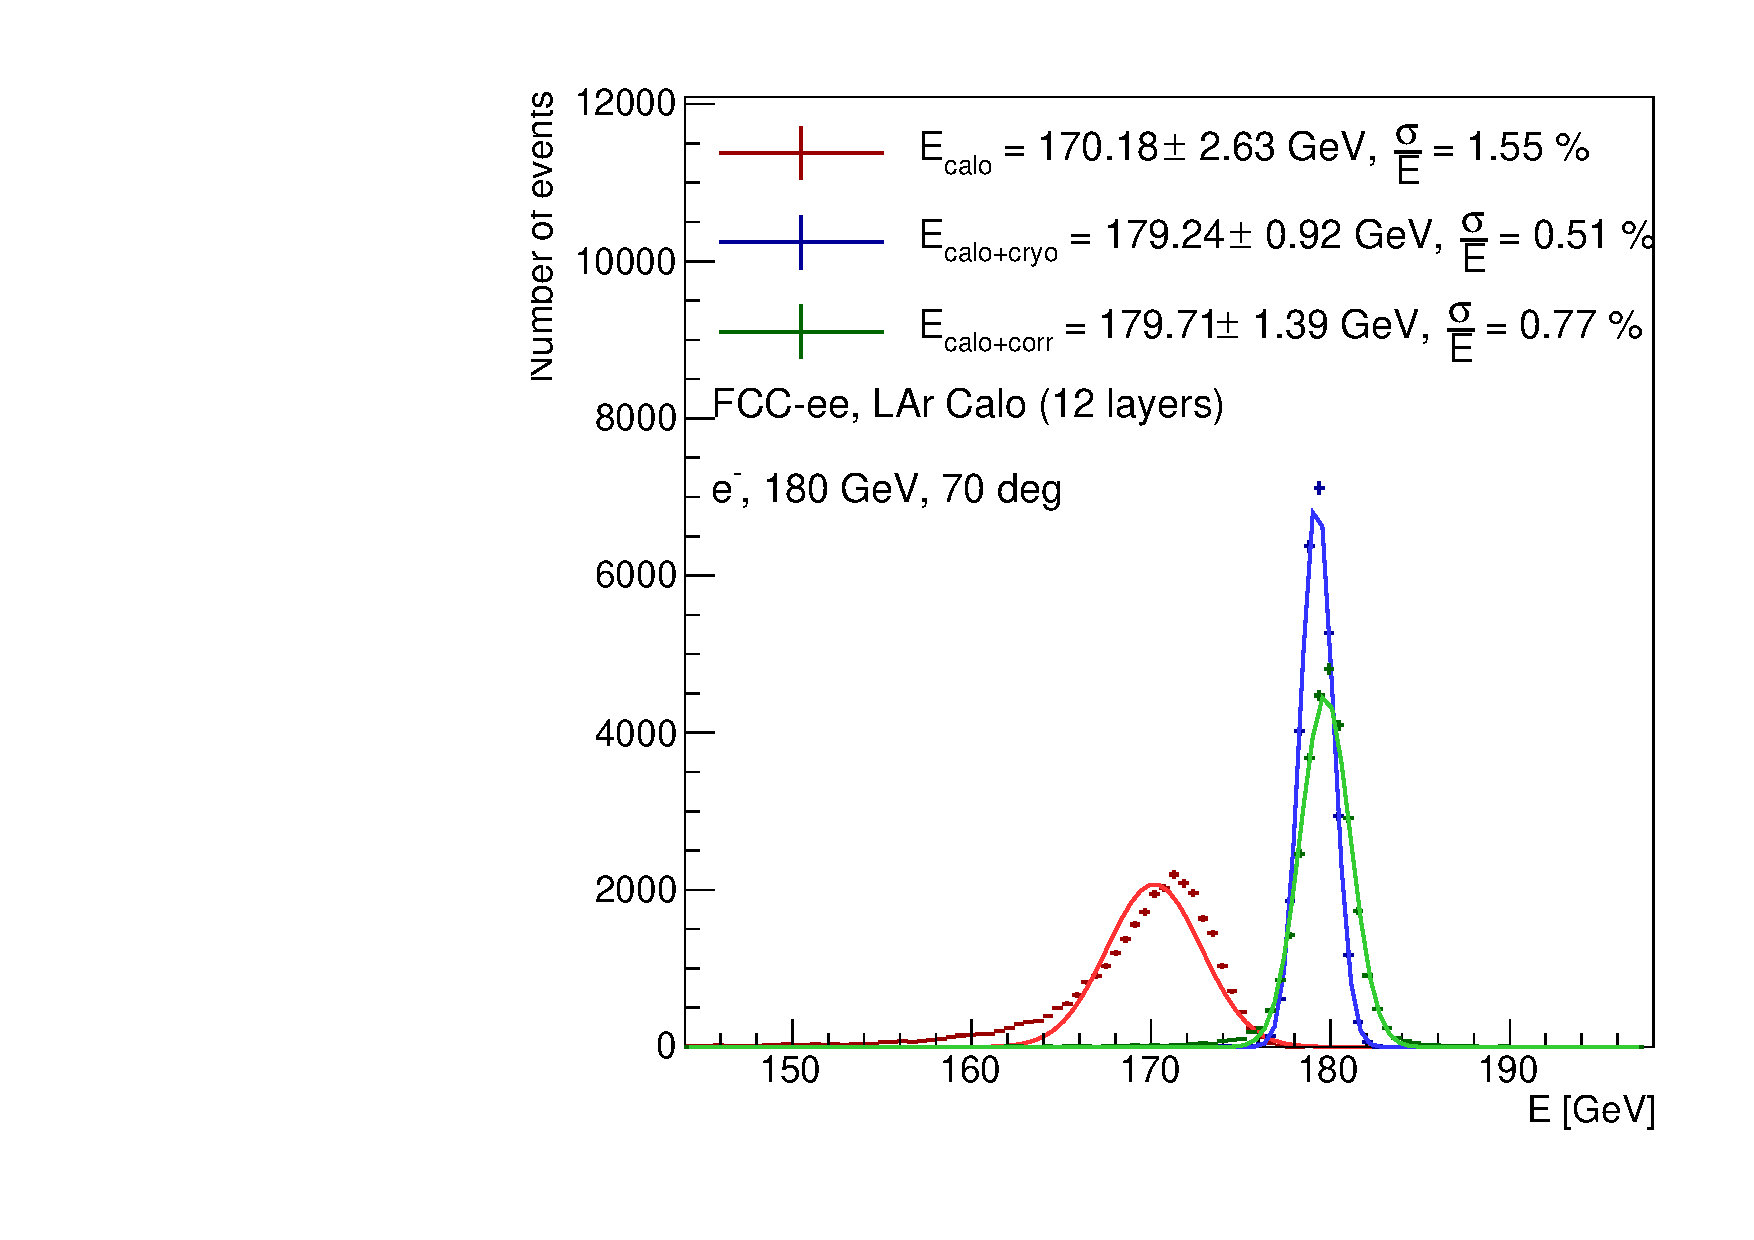
\includegraphics[width=0.49\linewidth]{figures/2d/hist_energy_corr_test_70deg_180GeV.pdf}
  \end{adjustwidth}
\end{frame}

\begin{frame}
  \frametitle{FCC-ee: Energy correction test IV.}

  \centering
  \begin{adjustwidth}{-5mm}{-5mm}
    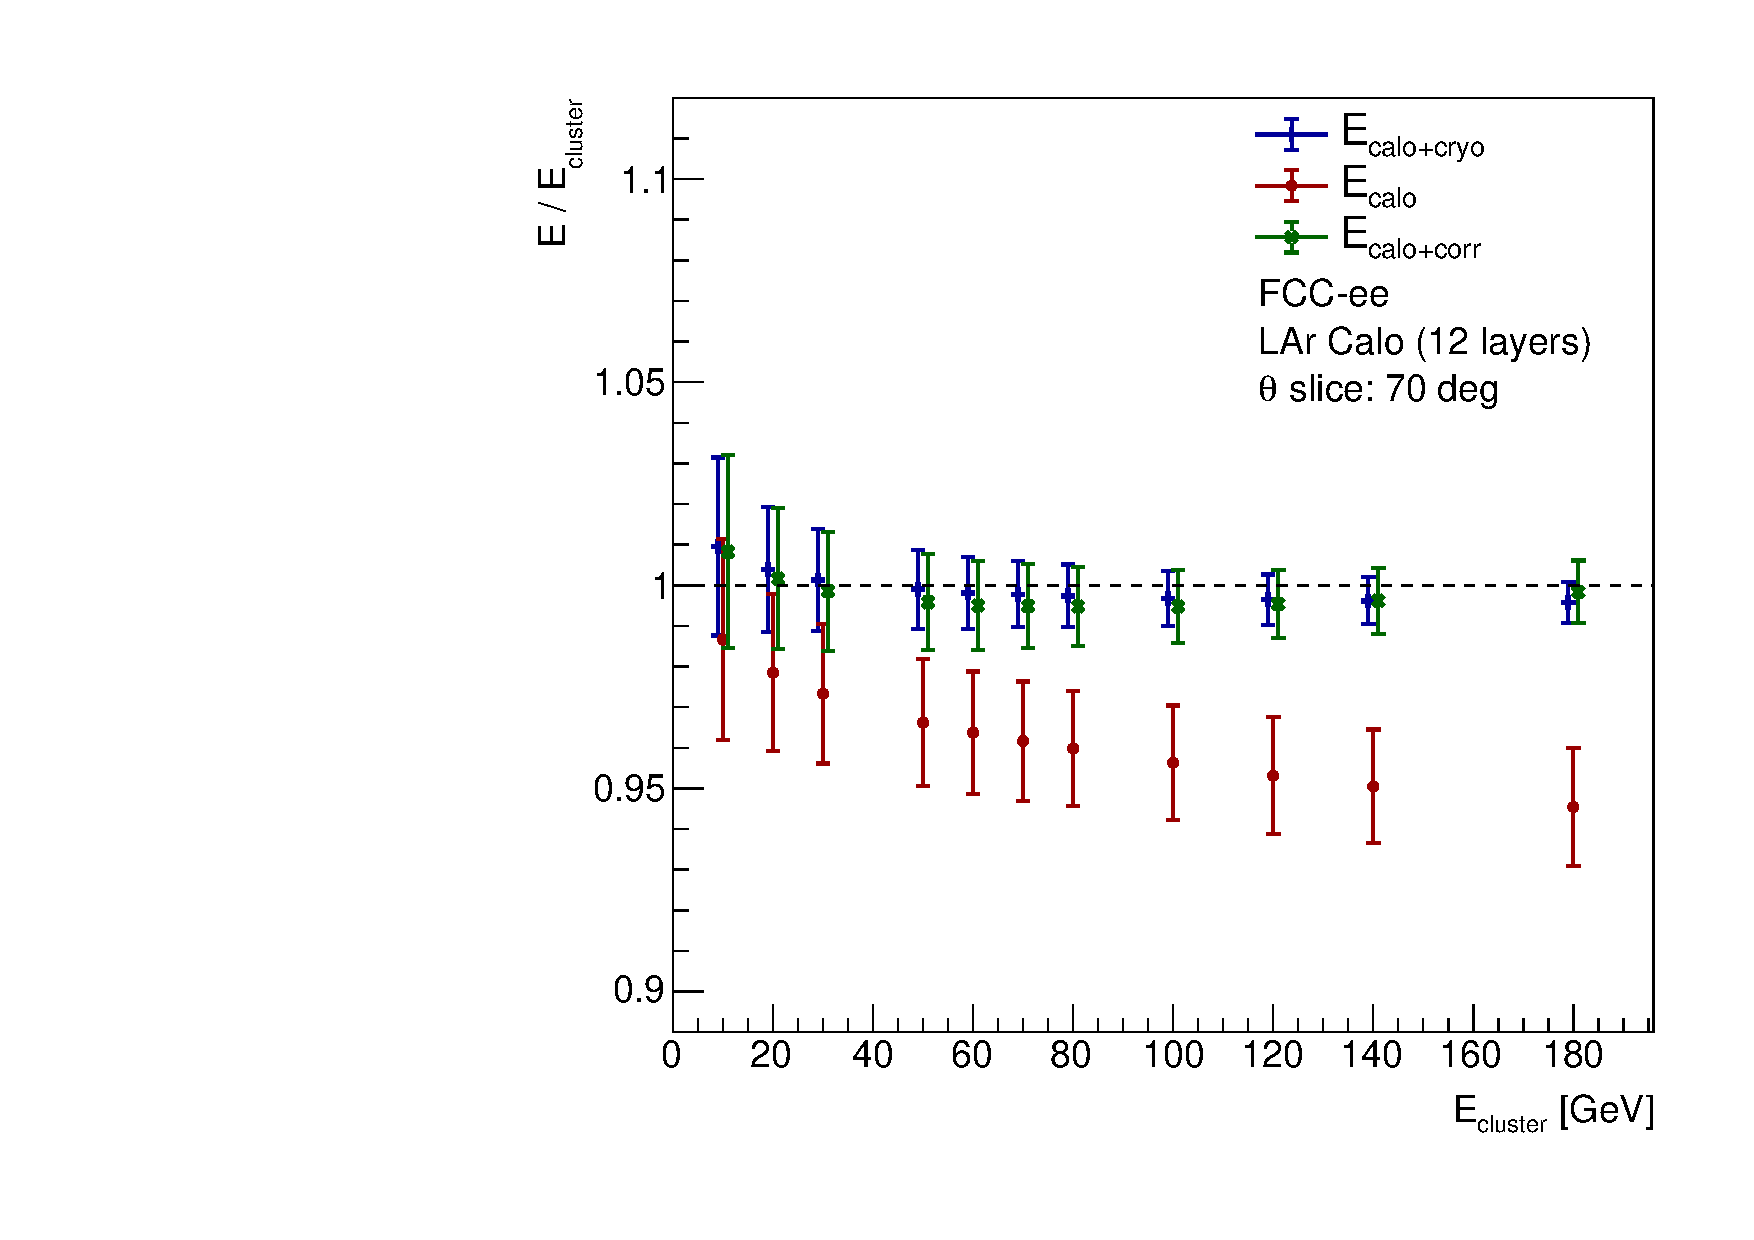
\includegraphics[width=0.49\linewidth]{figures/2d/graph_test_summary_mean_energy_70deg.pdf}
    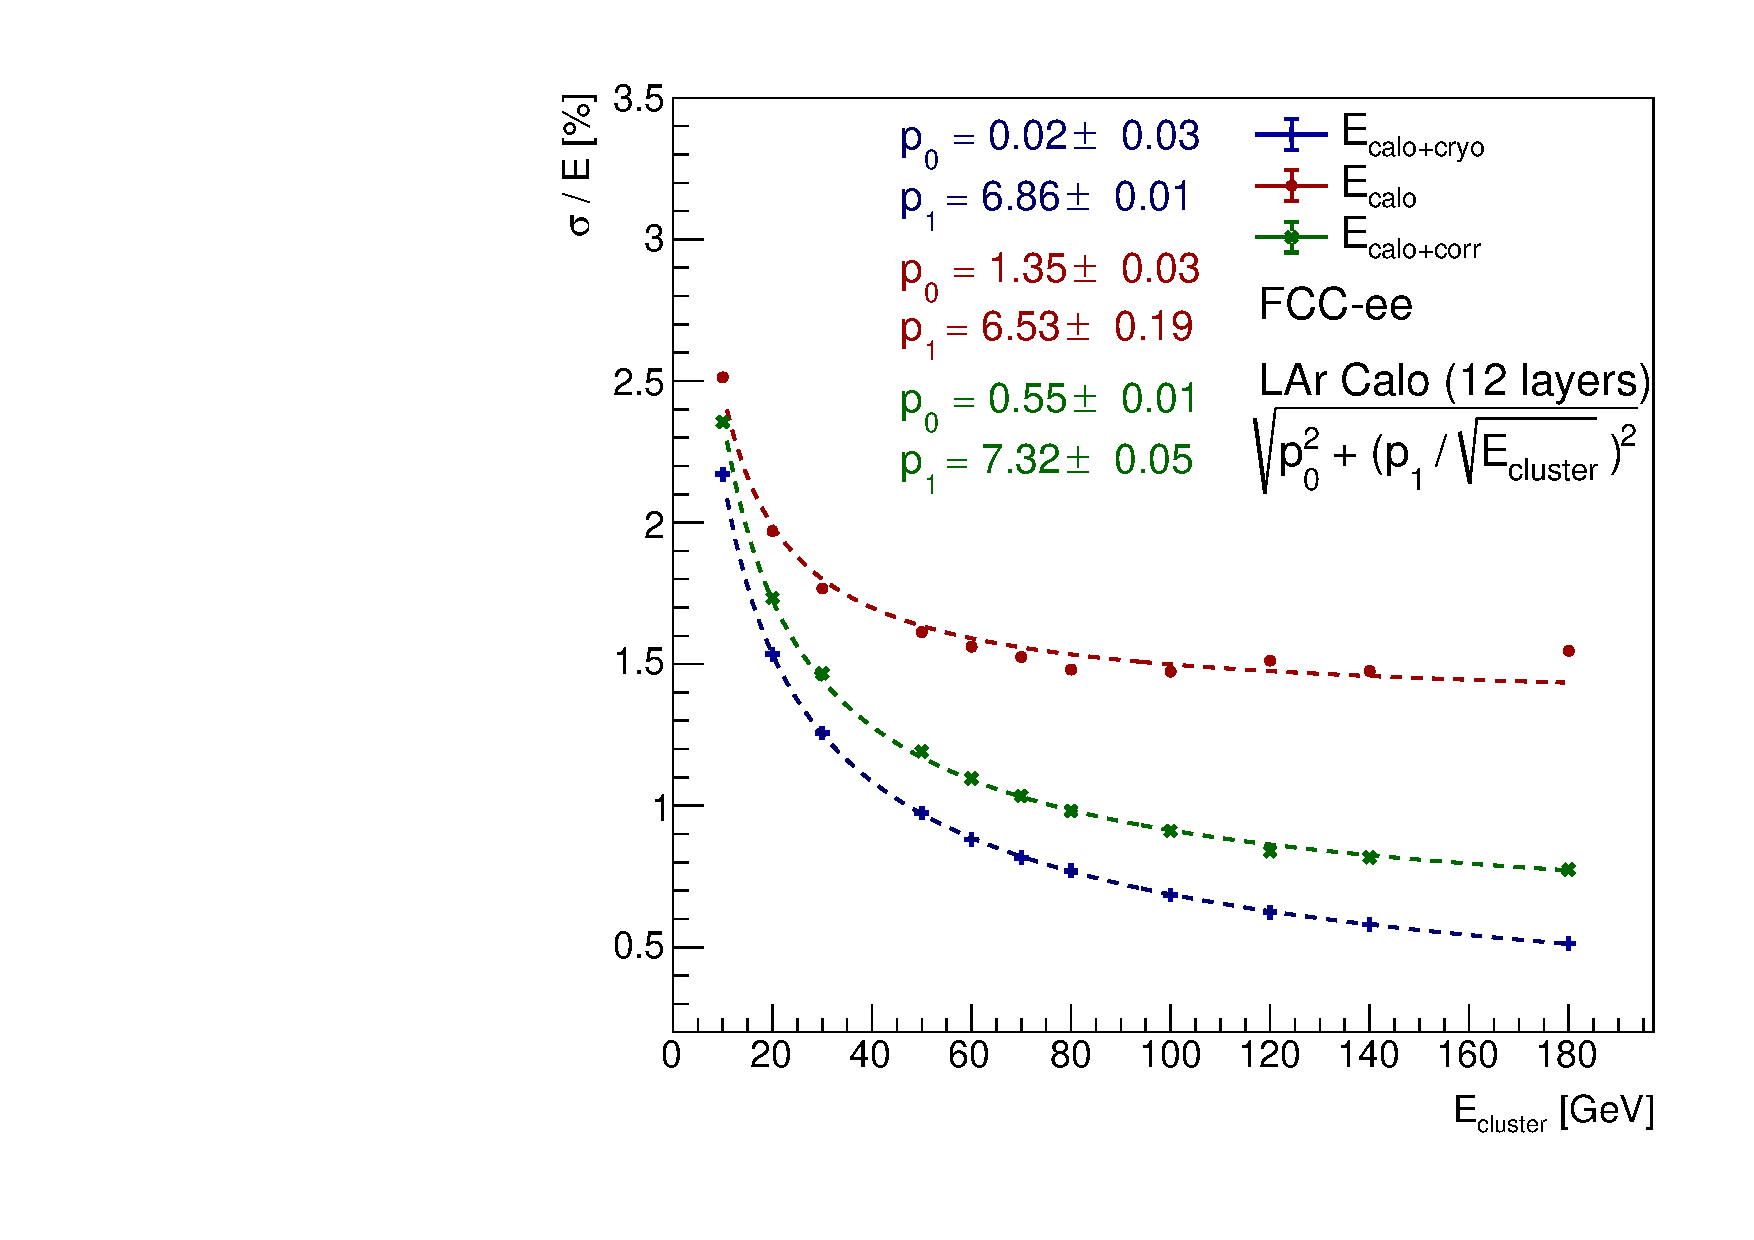
\includegraphics[width=0.49\linewidth]{figures/2d/graph_test_summary_res_energy_70deg.pdf}
  \end{adjustwidth}
\end{frame}

\begin{frame}
  \frametitle{FCC-ee: Energy correction test V.}

  \centering
  Only $E_{cluster}$ dependence \hspace{30mm}
  $\theta$ and $E_{cluster}$ dependence \\[1.5ex]
  \begin{adjustwidth}{-5mm}{-5mm}
    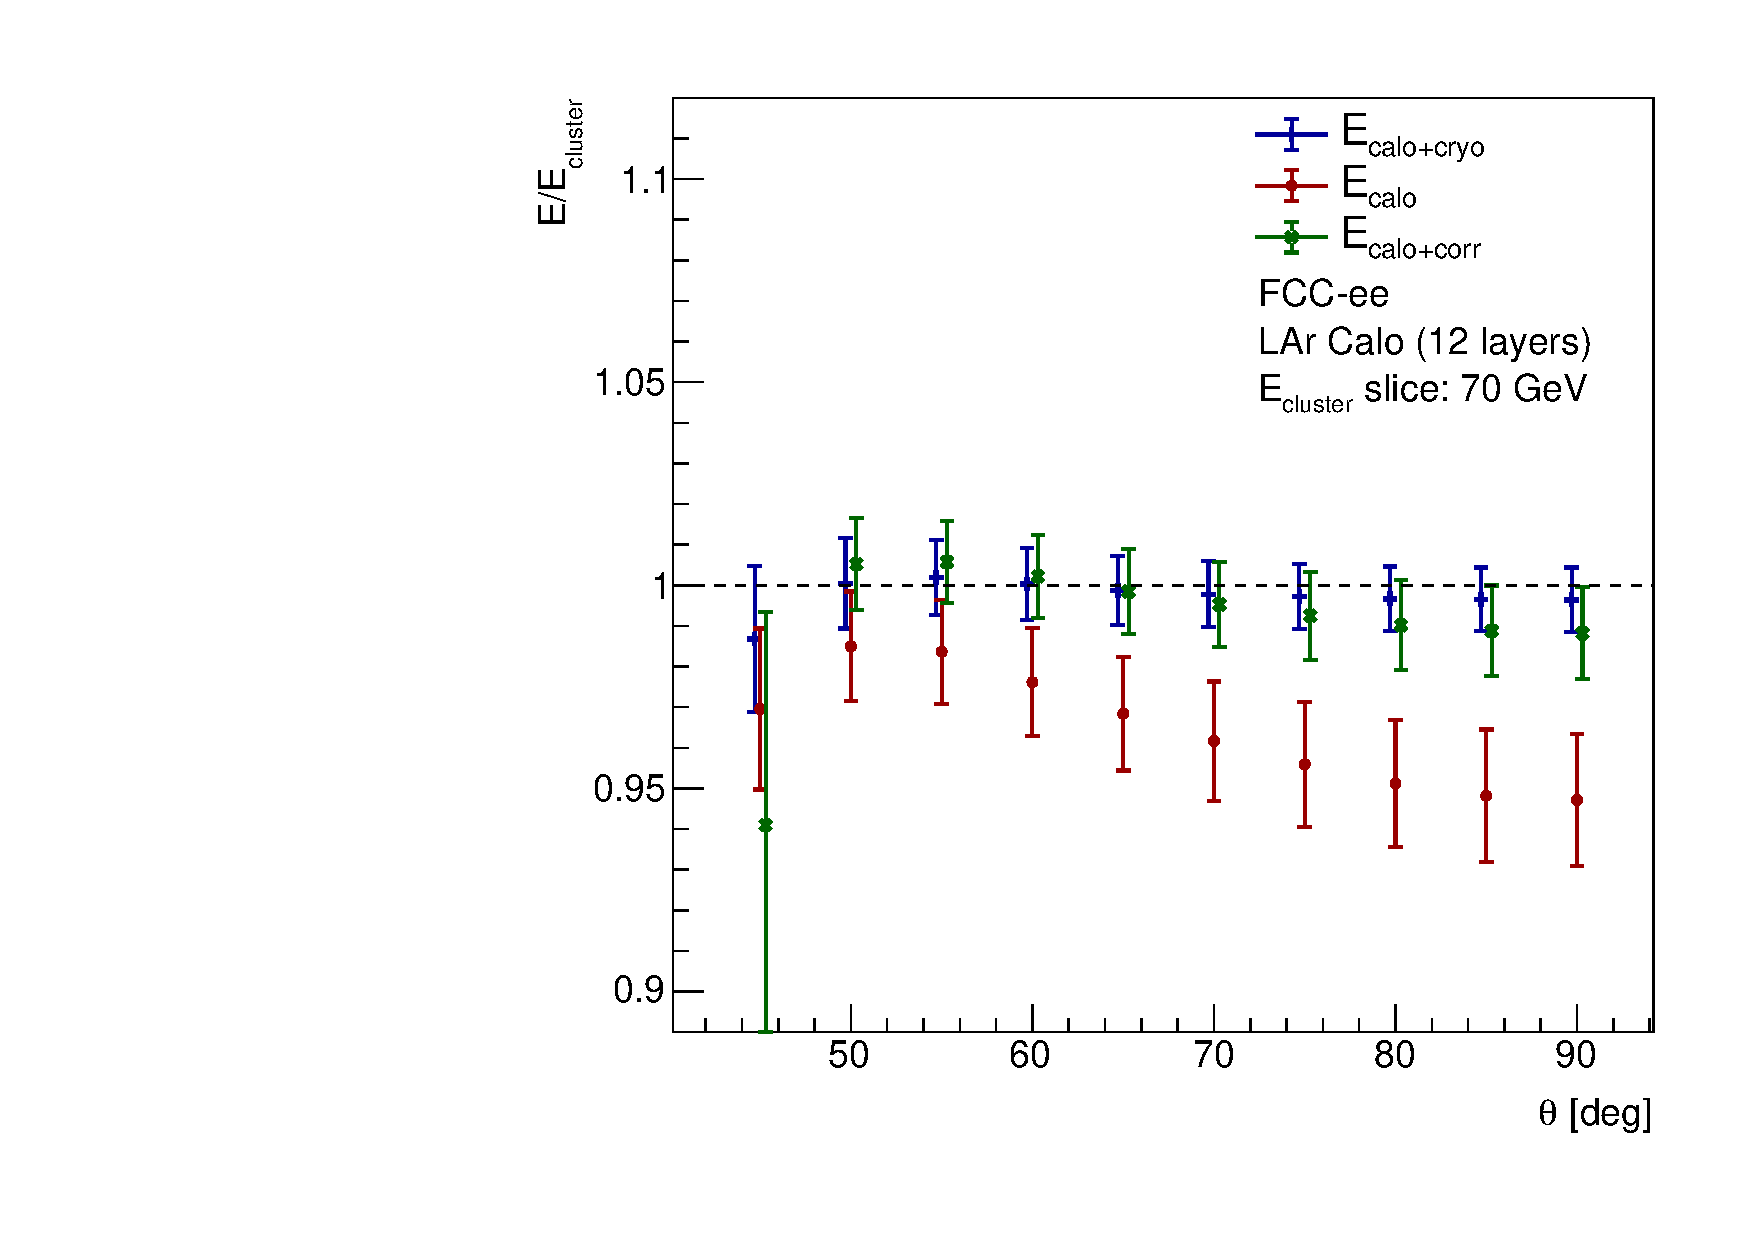
\includegraphics[width=0.49\linewidth]{figures/2d/graph_test_summary_mean_theta_70gev_1d.pdf}
    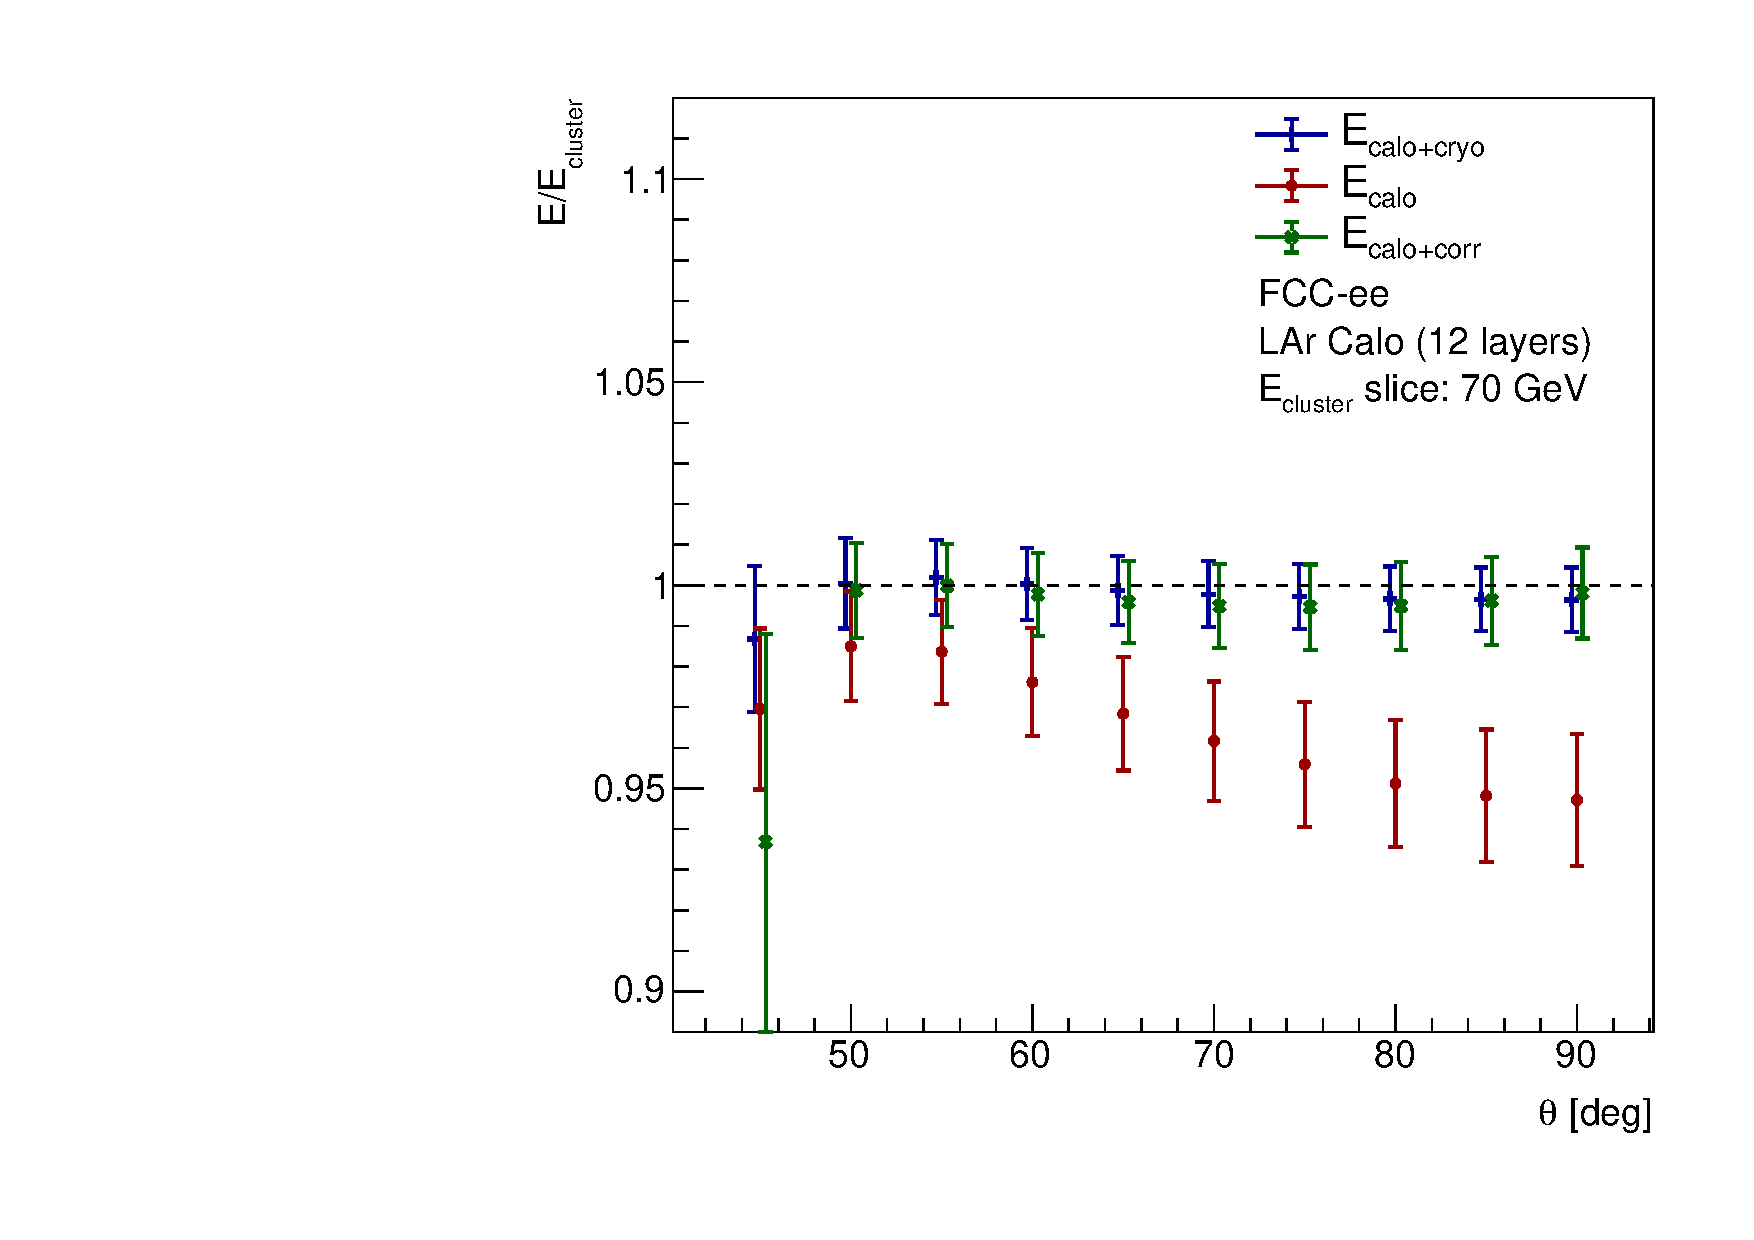
\includegraphics[width=0.49\linewidth]{figures/2d/graph_test_summary_mean_theta_70gev.pdf}
  \end{adjustwidth}
\end{frame}


% ---------------------------------------------------------------------------- %
\section{Conclusions and Plans}

\begin{frame}
  \frametitle{Conclusion and Plans}

  \begin{itemize}
    \item For FCC-ee large energy leakage observed
    \item Correlation between first/last layer and back cryostat exploited to create
          up/downstream corrections
    \item \redtext{Upstream} energy vs.\ energy in first layer \redtext{linear}
    \item \redtext{Downstream} energy vs.\ energy in last layer
          \redtext{quadratic}
    \item Parametrization can use any basic 1D/2D ROOT function
    \item Energy correction reconstructs cluster energy in whole energy and
          theta range
    \item \redtext{Inclusion of cluster theta dependence needed}
    \item \bluetext{\bf Links:}
          \begin{itemize}
            \item \href{https://github.com/kjvbrt/FCCSW/tree/calo_corr}
                  {\footnotesize \bluetext{\texttt{calo\_corr}: https://github.com/kjvbrt/FCCSW/tree/calo\_corr}}
            \item {\footnotesize \bluetext{Correction lives in: \texttt{Detector/DetStudies/scripts}}}
            \item \href{https://github.com/kjvbrt/FCCSW/tree/calo_corr_12}
                  {\scriptsize \bluetext{\texttt{calo\_corr\_12}: https://github.com/kjvbrt/FCCSW/tree/calo\_corr\_12}}
          \end{itemize}
  \end{itemize}
\end{frame}


% \appendix
% \backupbegin{}
%
% \begin{frame}[c]
%   \begin{center}
%     \redtext{\Huge Backup}
%   \end{center}
% \end{frame}
%
% \backupend{}

\end{document}
